% -*- Mode:TeX -*-

%% IMPORTANT: The official thesis specifications are available at:
%%            http://libraries.mit.edu/archives/thesis-specs/
%%
%%            Please verify your thesis' formatting and copyright
%%            assignment before submission.  If you notice any
%%            discrepancies between these templates and the 
%%            MIT Libraries' specs, please let us know
%%            by e-mailing thesis@mit.edu

%% The documentclass options along with the pagestyle can be used to generate
%% a technical report, a draft copy, or a regular thesis.  You may need to
%% re-specify the pagestyle after you \include  cover.tex.  For more
%% information, see the first few lines of mitthesis.cls. 

%\documentclass[12pt,vi,twoside]{mitthesis}
%%
%%  If you want your thesis copyright to you instead of MIT, use the
%%  ``vi'' option, as above.
%%
%\documentclass[12pt,twoside,leftblank]{mitthesis}
%%
%% If you want blank pages before new chapters to be labelled ``This
%% Page Intentionally Left Blank'', use the ``leftblank'' option, as
%% above. 

\documentclass[12pt,twoside]{mitthesis}
\usepackage{lgrind}
%% These have been added at the request of the MIT Libraries, because
%% some PDF conversions mess up the ligatures.  -LB, 1/22/2014
\usepackage{cmap}
\usepackage[T1]{fontenc}
\pagestyle{plain}

\usepackage{graphicx}
\usepackage[utf8]{inputenc}
\usepackage[T1]{fontenc} 
%\usepackage[latin1]{inputenc}
\usepackage{pifont} 
\usepackage{import}
\usepackage{amsmath}
\usepackage{multirow}
\usepackage{graphicx,url}
\usepackage{placeins}
\usepackage{adjustbox}
\usepackage[english]{babel}
\usepackage{lipsum}
\usepackage{multicol}
\usepackage{textcomp}
\usepackage{listings}
\usepackage[svgnames]{xcolor} 
\usepackage{caption}
\usepackage{amsmath}
\usepackage{calc} 
\usepackage{array,url,kantlipsum}
\usepackage{algorithm}
\usepackage{algpseudocode}
\usepackage{lscape}
\usepackage{array}
\usepackage{longtable}
\usepackage{booktabs}
\usepackage{txfonts}
\usepackage{colortbl}%
  \newcommand{\myrowcolour}{\rowcolor[gray]{0.925}}
\newenvironment{Figure}
  {\par\medskip\noindent\minipage{\linewidth}}
  {\endminipage\par\medskip}
  
\lstset{
language=Java,
basicstyle=\small\ttfamily,
numbers=left,
numbersep=5pt,
xleftmargin=20pt,
frame=tb,
framexleftmargin=20pt
}

\renewcommand*\thelstnumber{\arabic{lstnumber}:}

\DeclareCaptionFormat{mylst}{\hrule#1#2#3}
\captionsetup[lstlisting]{format=mylst,labelfont=bf,singlelinecheck=off,labelsep=space,font={normalsize,tt}}

\usepackage[framemethod=tikz]{mdframed}
\usepackage{lipsum}


%% This bit allows you to either specify only the files which you wish to
%% process, or `all' to process all files which you \include.
%% Krishna Sethuraman (1990).

%\typein [\files]{Enter file names to process, (chap1,chap2 ...), or `all' to
%process all files:}
%\def\all{all}
%\ifx\files\all \typeout{Including all files.} \else %\typeout{Including only \files.} \includeonly{\files} \fi

\newmdenv[innerlinewidth=0.5pt, roundcorner=4pt,innerleftmargin=6pt,
innerrightmargin=6pt,innertopmargin=6pt,innerbottommargin=6pt]{mybox}


\usepackage{titlesec}
\newcommand*{\justifyheading}{\raggedleft}
\titleformat{\chapter}[display]
  {\normalfont\huge\bfseries\justifyheading}{\chaptertitlename\ \thechapter}
  {20pt}{\Huge}[{\titlerule[0.8pt]}]

\begin{document}

% -*-latex-*-
% 
% For questions, comments, concerns or complaints:
% thesis@mit.edu
% 
%
% $Log: cover.tex,v $
% Revision 1.8  2008/05/13 15:02:15  jdreed
% Degree month is June, not May.  Added note about prevdegrees.
% Arthur Smith's title updated
%
% Revision 1.7  2001/02/08 18:53:16  boojum
% changed some \newpages to \cleardoublepages
%
% Revision 1.6  1999/10/21 14:49:31  boojum
% changed comment referring to documentstyle
%
% Revision 1.5  1999/10/21 14:39:04  boojum
% *** empty log message ***
%
% Revision 1.4  1997/04/18  17:54:10  othomas
% added page numbers on abstract and cover, and made 1 abstract
% page the default rather than 2.  (anne hunter tells me this
% is the new institute standard.)
%
% Revision 1.4  1997/04/18  17:54:10  othomas
% added page numbers on abstract and cover, and made 1 abstract
% page the default rather than 2.  (anne hunter tells me this
% is the new institute standard.)
%
% Revision 1.3  93/05/17  17:06:29  starflt
% Added acknowledgements section (suggested by tompalka)
% 
% Revision 1.2  92/04/22  13:13:13  epeisach
% Fixes for 1991 course 6 requirements
% Phrase "and to grant others the right to do so" has been added to 
% permission clause
% Second copy of abstract is not counted as separate pages so numbering works
% out
% 
% Revision 1.1  92/04/22  13:08:20  epeisach

% NOTE:
% These templates make an effort to conform to the MIT Thesis specifications,
% however the specifications can change.  We recommend that you verify the
% layout of your title page with your thesis advisor and/or the MIT 
% Libraries before printing your final copy.
\title{Improving Stress Search Based Testing using Q-Learning and Hybrid Metaheuristic Approach}

\author{Francisco Nauber Bernardo Gois}
% If you wish to list your previous degrees on the cover page, use the 
% previous degrees command:
%       \prevdegrees{A.A., Harvard University (1985)}
% You can use the \\ command to list multiple previous degrees
%       \prevdegrees{B.S., University of California (1978) \\
%                    S.M., Massachusetts Institute of Technology (1981)}
\department{Department of Electrical Engineering and Computer Science}

% If the thesis is for two degrees simultaneously, list them both
% separated by \and like this:
% \degree{Doctor of Philosophy \and Master of Science}
\degree{Doctor of Science in Computer Science and Engineering}

% As of the 2007-08 academic year, valid degree months are September, 
% February, or June.  The default is June.
\degreemonth{February}
\degreeyear{2017}
\thesisdate{February 16, 2017}

%% By default, the thesis will be copyrighted to MIT.  If you need to copyright
%% the thesis to yourself, just specify the `vi' documentclass option.  If for
%% some reason you want to exactly specify the copyright notice text, you can
%% use the \copyrightnoticetext command.  
%\copyrightnoticetext{\copyright IBM, 1990.  Do not open till Xmas.}

% If there is more than one supervisor, use the \supervisor command
% once for each.
\supervisor{William J. Dally}{Associate Professor}

% This is the department committee chairman, not the thesis committee
% chairman.  You should replace this with your Department's Committee
% Chairman.
\chairman{Arthur C. Smith}{Chairman, Department Committee on Graduate Theses}

% Make the titlepage based on the above information.  If you need
% something special and can't use the standard form, you can specify
% the exact text of the titlepage yourself.  Put it in a titlepage
% environment and leave blank lines where you want vertical space.
% The spaces will be adjusted to fill the entire page.  The dotted
% lines for the signatures are made with the \signature command.
\maketitle

% The abstractpage environment sets up everything on the page except
% the text itself.  The title and other header material are put at the
% top of the page, and the supervisors are listed at the bottom.  A
% new page is begun both before and after.  Of course, an abstract may
% be more than one page itself.  If you need more control over the
% format of the page, you can use the abstract environment, which puts
% the word "Abstract" at the beginning and single spaces its text.

%% You can either \input (*not* \include) your abstract file, or you can put
%% the text of the abstract directly between the \begin{abstractpage} and
%% \end{abstractpage} commands.

% First copy: start a new page, and save the page number.
\cleardoublepage
% Uncomment the next line if you do NOT want a page number on your
% abstract and acknowledgments pages.
% \pagestyle{empty}
\setcounter{savepage}{\thepage}
\begin{abstractpage}
% $Log: abstract.tex,v $
% Revision 1.1  93/05/14  14:56:25  starflt
% Initial revision
% 
% Revision 1.1  90/05/04  10:41:01  lwvanels
% Initial revision
% 
%
%% The text of your abstract and nothing else (other than comments) goes here.
%% It will be single-spaced and the rest of the text that is supposed to go on
%% the abstract page will be generated by the abstractpage environment.  This
%% file should be \input (not \include 'd) from cover.tex.
In this thesis, I designed and implemented a compiler which performs
optimizations that reduce the number of low-level floating point operations
necessary for a specific task; this involves the optimization of chains of
floating point operations as well as the implementation of a ``fixed'' point
data type that allows some floating point operations to simulated with integer
arithmetic.  The source language of the compiler is a subset of C, and the
destination language is assembly language for a micro-floating point CPU.  An
instruction-level simulator of the CPU was written to allow testing of the
code.  A series of test pieces of codes was compiled, both with and without
optimization, to determine how effective these optimizations were.

\end{abstractpage}

% Additional copy: start a new page, and reset the page number.  This way,
% the second copy of the abstract is not counted as separate pages.
% Uncomment the next 6 lines if you need two copies of the abstract
% page.
% \setcounter{page}{\thesavepage}
% \begin{abstractpage}
% % $Log: abstract.tex,v $
% Revision 1.1  93/05/14  14:56:25  starflt
% Initial revision
% 
% Revision 1.1  90/05/04  10:41:01  lwvanels
% Initial revision
% 
%
%% The text of your abstract and nothing else (other than comments) goes here.
%% It will be single-spaced and the rest of the text that is supposed to go on
%% the abstract page will be generated by the abstractpage environment.  This
%% file should be \input (not \include 'd) from cover.tex.
In this thesis, I designed and implemented a compiler which performs
optimizations that reduce the number of low-level floating point operations
necessary for a specific task; this involves the optimization of chains of
floating point operations as well as the implementation of a ``fixed'' point
data type that allows some floating point operations to simulated with integer
arithmetic.  The source language of the compiler is a subset of C, and the
destination language is assembly language for a micro-floating point CPU.  An
instruction-level simulator of the CPU was written to allow testing of the
code.  A series of test pieces of codes was compiled, both with and without
optimization, to determine how effective these optimizations were.

% \end{abstractpage}

\cleardoublepage

\section*{Acknowledgments}

This is the acknowledgements section.  You should replace this with your
own acknowledgements.

%%%%%%%%%%%%%%%%%%%%%%%%%%%%%%%%%%%%%%%%%%%%%%%%%%%%%%%%%%%%%%%%%%%%%%
% -*-latex-*-

\section*{Related Publications}


The following publications are related to this thesis:

\begin{itemize}
\item \textbf{N. Gois, P. Porfirio, A. Coelho, and T. Barbosa}. Improving Stress Search Based Testing using a Hybrid Metaheuristic Approach. In Proceedings of the 2016 Latin American Computing Conference (CLEI), pages 718–728, 2016 \cite{Gois2016}.
\end{itemize}

% Some departments (e.g. 5) require an additional signature page.  See
% signature.tex for more information and uncomment the following line if
% applicable.
% % -*- Mode:TeX -*-
%
% Some departments (e.g. Chemistry) require an additional cover page
% with signatures of the thesis committee.  Please check with your
% thesis advisor or other appropriate person to determine if such a 
% page is required for your thesis.  
%
% If you choose not to use the "titlepage" environment, a \newpage
% commands, and several \vspace{\fill} commands may be necessary to
% achieve the required spacing.  The \signature command is defined in
% the "mitthesis" class
%
% The following sample appears courtesy of Ben Kaduk <kaduk@mit.edu> and
% was used in his June 2012 doctoral thesis in Chemistry. 

\begin{titlepage}
\begin{large}
This doctoral thesis has been examined by a Committee of the Department
of Chemistry as follows:

\signature{Professor Jianshu Cao}{Chairman, Thesis Committee \\
   Professor of Chemistry}

\signature{Professor Troy Van Voorhis}{Thesis Supervisor \\
   Associate Professor of Chemistry}

\signature{Professor Robert W. Field}{Member, Thesis Committee \\
   Haslam and Dewey Professor of Chemistry}
\end{large}
\end{titlepage}


\pagestyle{plain}
  % -*- Mode:TeX -*-
%% This file simply contains the commands that actually generate the table of
%% contents and lists of figures and tables.  You can omit any or all of
%% these files by simply taking out the appropriate command.  For more
%% information on these files, see appendix C.3.3 of the LaTeX manual. 
\tableofcontents
\newpage
\listoffigures
\newpage
\listoftables


%% This is an example first chapter.  You should put chapter/appendix that you
%% write into a separate file, and add a line \include{yourfilename} to
%% main.tex, where `yourfilename.tex' is the name of the chapter/appendix file.
%% You can process specific files by typing their names in at the 
%% \files=
%% prompt when you run the file main.tex through LaTeX.
\chapter{Introduction}

Many systems must support concurrent access by hundreds or thousands of users. Failure to providing scalable access to users may results in catastrophic failures and unfavorable media coverage \cite{Jiang2010}. 

The explosive growth of the Internet has contributed to the increased need for applications that perform at an appropriate speed. Performance problems are often detected late in the application life cycle, and the later they are discovered, the greater the cost to fix them \cite{Molyneaux2009}.

The use of stress testing is an increasingly common practice owing to the increasing number of users. In this scenario, the inadequate treatment of a workload generated by concurrent or simultaneous access due to several users can result in highly critical failures and negatively affect the customers perception of the company \cite{Draheim2006b} \cite{Jiang2010}. 

Stress testing determines the responsiveness, throughput, reliability, or scalability of a system under a given workload. The quality of the results of applying a given load testing to a system is closely linked to the implementation of the workload strategy. The performance of many applications depends on the load applied under different conditions. In some cases, performance degradation and failures arise only in stress conditions \cite{Garousi2010} \cite{Jiang2010}.


A stress test uses a set of workloads that consist of many types of usage scenarios and a combination of different numbers of users. A load is typically based on an operational profile. Different parts of an application should be tested under various parameters and stress conditions \cite{Babbar2011}. The correct application of a stress test should cover most parts of an application above the expected load conditions\cite{Draheim2006b}.


Fig. \ref{fig:example} shows an example of a system under assessment with three pages (the main page, profile page, and search page) and six possible users. From the combinations of users and application pages, various scenarios can be created, such as scenarios 1 and 2 shown in the figure. The first scenario presents a test that has passed, and the second scenario presents a test that has an HTTP 404 error.

\begin{figure}[ht]
\centering
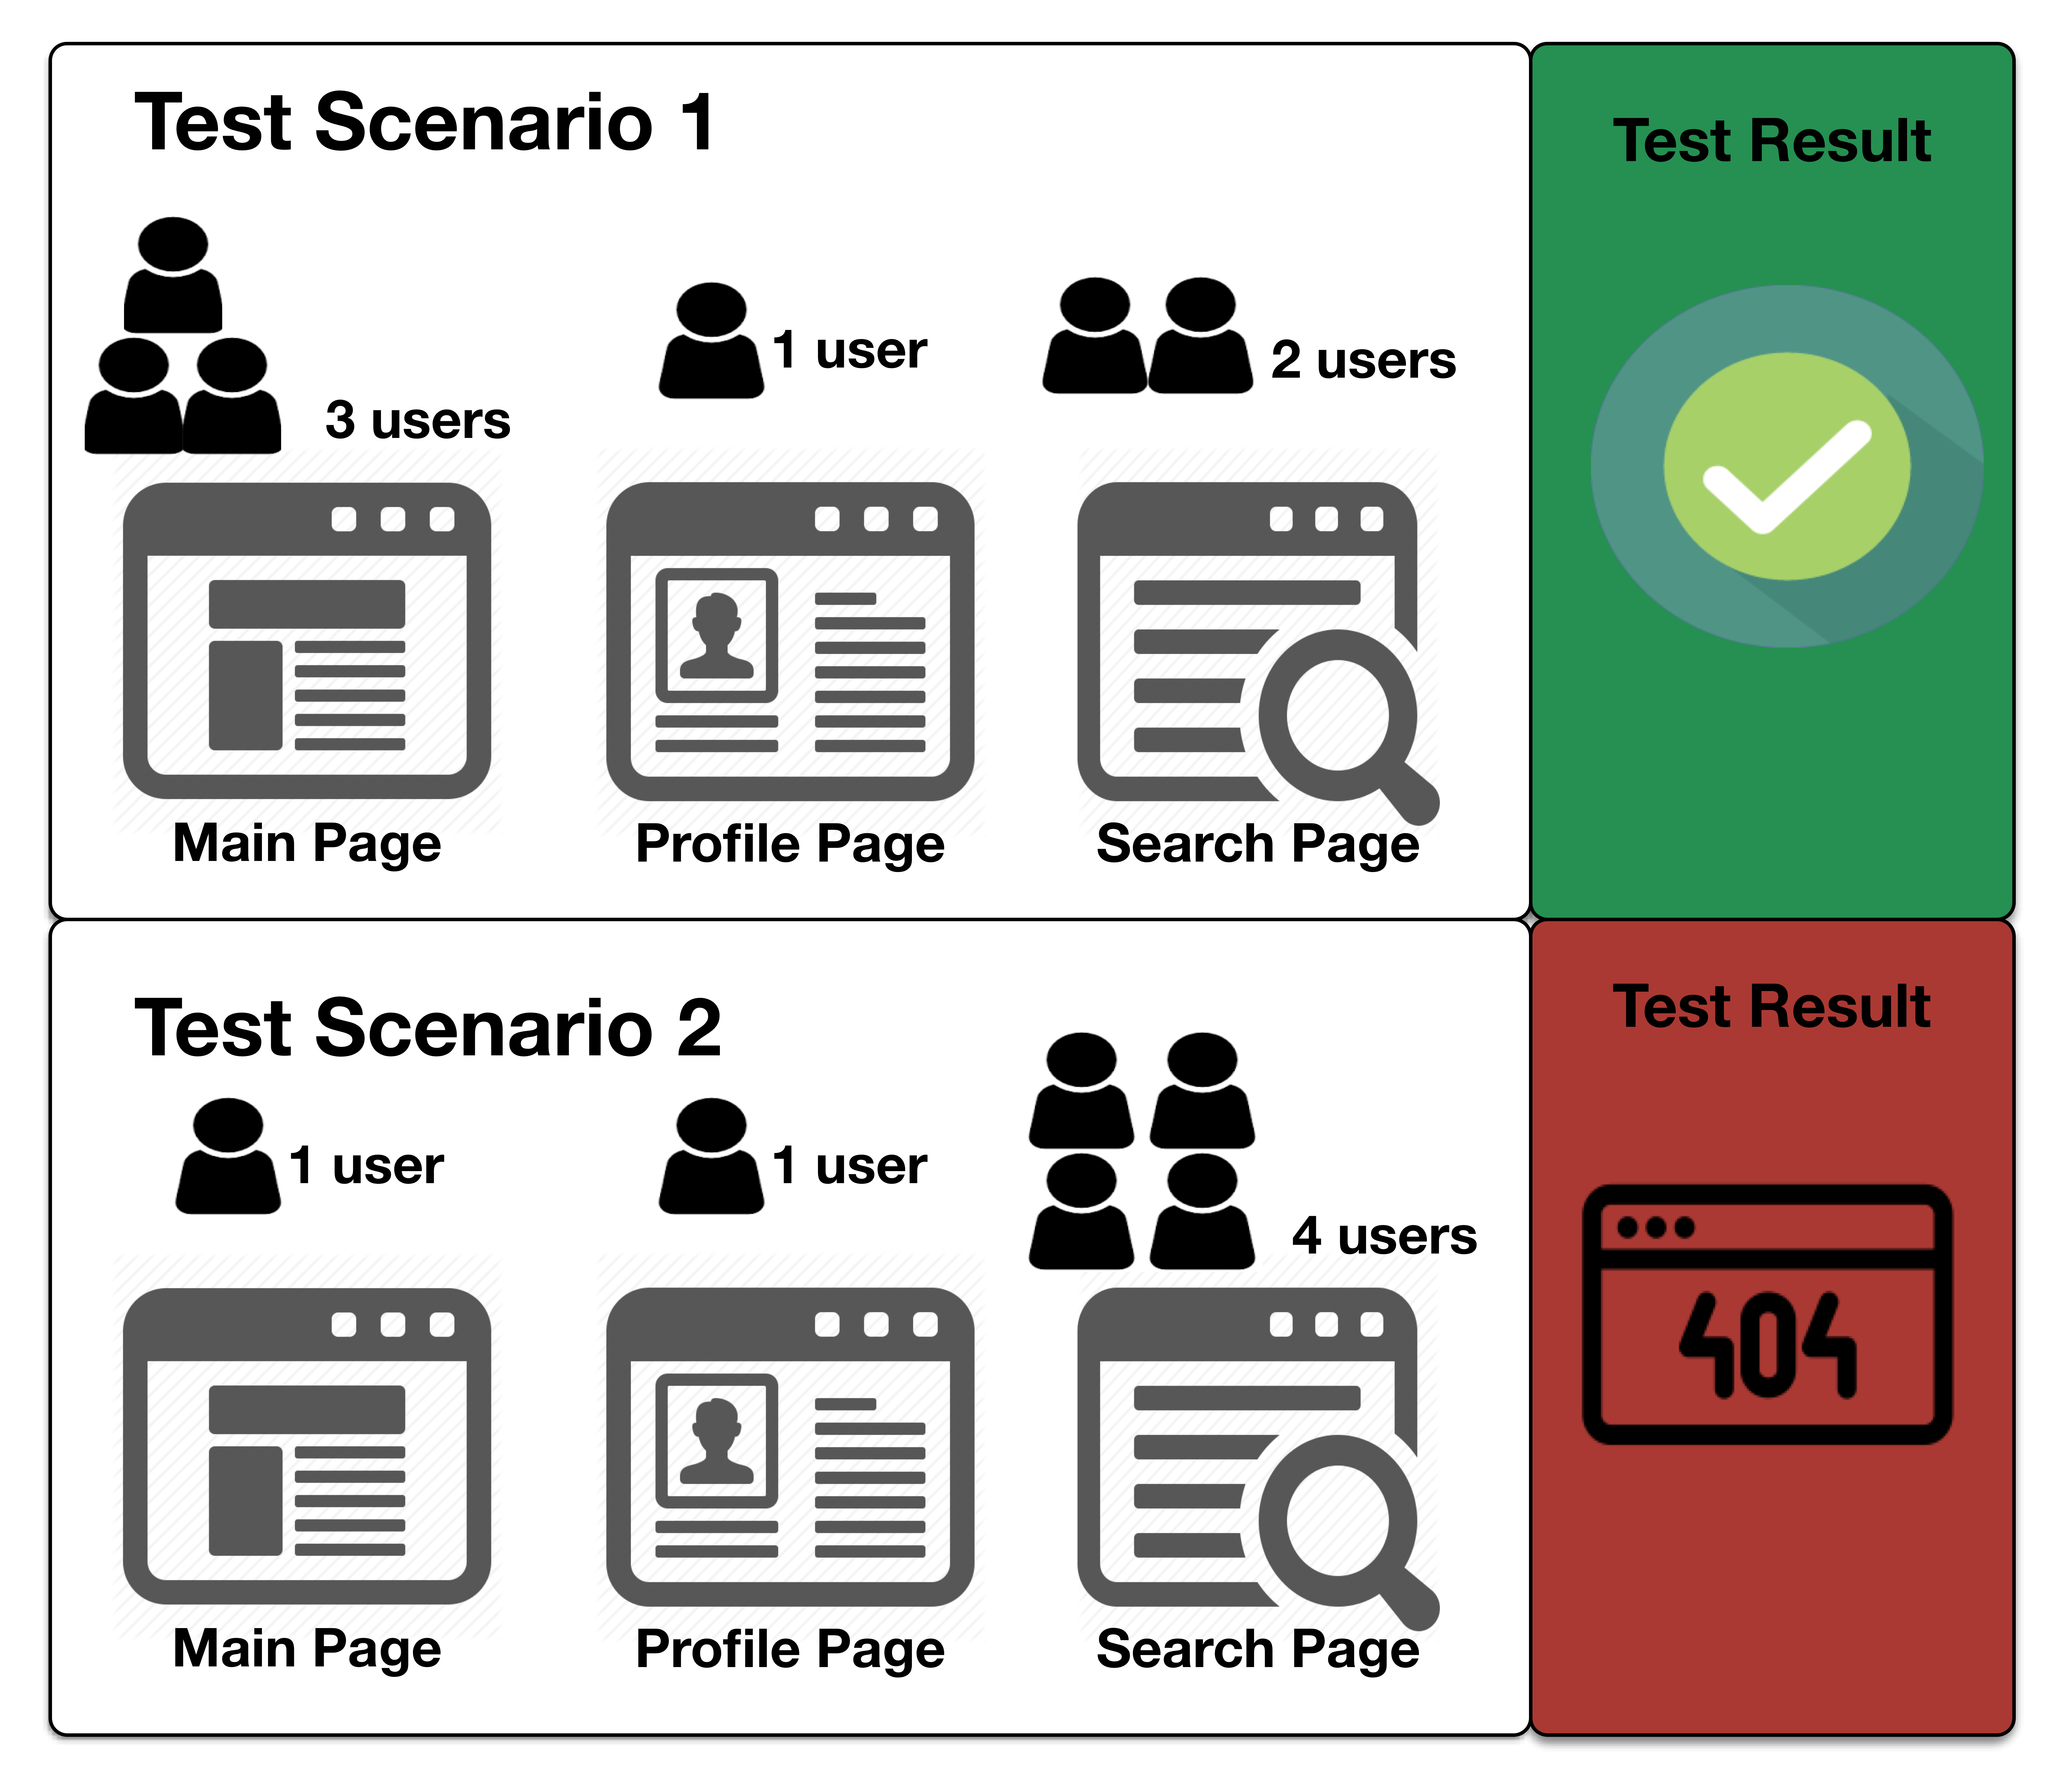
\includegraphics[width=0.4\textwidth]{./images/diagram.png}
\caption{Possible test scenarios for a hypothetical application}
\label{fig:example}
\end{figure}

A stress test usually lasts for several hours or even a few days and only tests a limited number of workloads. The major challenge is to find the workloads that expose a major number of errors and to discover the maximum number of users supported by an application under testing \cite{Barna2011}. 

Search-based testing is seen as a promising approach to verifying timing constraints \cite{Afzal2009a}. A common objective of a load search-based test is to find  scenarios that produce execution times that violate the specified timing constraints \cite{Sullivan}. 

\section{Motivation}

There is strong empirical evidence, that deficient
testing of both functional and nonfunctional properties
is one of the major sources of software and system errors. In 2002, NIST  report found that more than one-third of these costs of software failure could be eliminated by an improved testing infrastructure.
Automation of testing is a crucial concern. Through
automation, large-scale thorough testing can become
practical and scalable. However, the automated generation of test cases presents challenges. The general problem involves finding a (partial) solution to the path sensitization problem. That is, the problem of finding an input to drive the software down a chosen path \cite{Harman2010} \cite{dean2003managing}. 

Software performance is a pervasive quality, because it is affected by every aspect of the design, code, and execution environment. Performance failures occur when a software product is unable to meet its overall objectives due to inadequate performance. Such failures negatively impact the projects by increasing costs, decreasing revenue or both \cite{Vetoio2011}. 

Software testing is a expensive and difficult activity. The exponential
growth in the complexity of software makes the cost of testing has only continued to rise. Test case generation can be seen as a search problem. The test adequacy criterion is transformed into a fitness function and a set of solutions in the search
space are evaluated with respect to the fitness function using a metaheuristic search technique. Search-based software testing is the application of metaheuristic search techniques to generate software
tests cases or perform test execution \cite{Afzal2009a} \cite{Gay}.

Performance testing of enterprise applications is manual,laborious, costly, and not particulary effective. When running many different test cases and observing application’s behavior, testers intuitively sense that there are certain properties of test cases that are likely to reveal performance bugs. Distilling these properties automatically into rules that describe how these properties affect performance of the application is a subgoal of our approach \cite{Grechanik2012}.

Experimentation is important to realistically and accurately test and evaluate search based tests. Experimentation on algorithms is usually made by simulation. Experiments involving search based tests are inherently complex and typically time-consuming to set up and execute. Such experiments are also extremely difficult to repeat. People who might want to duplicate published results, for example, must devote substantial resources to setting up and the environmental conditions are likely to be substantially different.

Below we briefly describe the related research and practices on stress testing:



\subsection{State of Research on the Search-Based Stress  Testing}

In the academic context, a number of studies proving the efficacy of metaheuristics to automate test execution can be found in literature. A variety of metaheuristic search techniques are found to be applicable for non-functional testing including simulated annealing, tabu search, genetic algorithms, ant colony methods, grammatical evolution, genetic programming and swarm intelligence methods. Most research studies are limited to making prototype.  The presented research work is distinguished from others by having extend a industrial tool using a hybrid approach and q-learning \cite{Afzal2009a}.  

\subsection{State of Industrial Practices on Stress Tests}

The stress testing process in the industry still follows a non-automated and ad-hoc model where the designer or tester is responsible for running the tests analyzing the results and deciding which new tests should be performed \cite{Lewis2005}. 

Typically, performance testing is accomplished using test scripts, which are programs that test designers write to automate testing. These test scripts performs actions or mimicking user actions on GUI objects of the system to feed input data. Current approaches to load testing suffer from limitations. Their cost-effectiveness is highly dependent on the particular test scenarios that are used yet there is no support for choosing those scenarios. A poor choice of scenarios could lead to underestimating system response time thereby missing an opportunity to detect a performance \cite{Grechanik2012}.


\section{Research Hypothesis}





Our underlying research hypothesis is as follows:

\begin{mybox}
The use of metaheuristics and hybrid metaheuristics in combination with Q-learning can make it possible to automate the stress test execution process, improving the choice of new test cases for each interaction and finding scenarios that maximize the number of users of the application under test and minimize response time or find scenarios with a expected response time.
\end{mybox}

The purpose of this thesis is to show the validity of this hypothesis through the development of a testbed tool, algorithms that use hybrid metaheuristics and the Q-learning technique and application of validation experiments. This thesis will be useful for load test practitioners and software engineering researchers interested in large-scale testing software systems.


\section{Thesis Overview}

In this section, we present an overview of the works presented in this thesis. This thesis has five main chapters

\section{Thesis Contributions}

The major contributions of this thesis are:

\begin{itemize}
\item Hybrid Metaheuristic Approach \cite{Gois2016}: We present a hybrid metaheuristic approach that uses Genetic Algorithms, Simulated Annealing and Tabu Search  in a collaborative mode.

\item Q-Learning Metaheuristic Approach: 
\item IAdapter JMeter Plugin:
\item Testbed Tool: 
\end{itemize}




\section{Thesis Organization}



\chapter{A Survey on Stress Testing Software Systems}

Load, performance, and stress testing are typically done to locate bottlenecks in a system, to support a performance-tuning effort, and to collect other performance-related indicators to help stakeholders get informed about the quality of the application being tested \cite{Sandler2004} \cite{Corporation2007}. 


The performance testing aims at verifying a specified system performance. This kind of test is executed by simulating hundreds of simultaneous users or more over a defined time interval \cite{DiLucca2006}. The purpose of this assessment is to demonstrate that the system reaches its performance objectives \cite{Sandler2004}.  Term often used interchangeably with “stress” and “load” testing. Ideally “performance” testing is defined in requirements documentation or QA or Test Plans \cite{Lewis2005}.


In a load testing, the system is evaluated at predefined load levels \cite{DiLucca2006}. The aim of this test is to determine whether the system can reach its performance targets for availability, concurrency, throughput, and response time. Load testing is the closest to real application use \cite{Molyneaux2009}. A typical load test can last from several hours to a few days, during which system behavior data like execution logs and various metrics are collected \cite{Afzal2009a}. 

Stress testing investigates the behavior of the system under conditions
that overload its resources. The stress testing verifies the system behavior against heavy workloads \cite{Sandler2004} \cite{Lewis2005}, which are executed to evaluate a system beyond its limits, validate system response in activity peaks, and verify whether the system is able to recover from these conditions. It differs from other kinds of testing in that the system is executed on or beyond its breakpoints, forcing the application or the supporting infrastructure to fail \cite{DiLucca2006} \cite{Molyneaux2009}.


This chapter surveys the state of the art literature in stress testing research. This survey will be useful for stress testing practitioners and software engineering researchers with interests in testing and analyzing software systems. We proposed the following three research questions:


\begin{itemize}
\item How is a proper stress designed?
\item How is a stress test executed and automated?
\item What are the main problems found by stress tests?
\end{itemize}

The population in this study is the domain of software testing. Intervention includes application of stress test techniques to test different types of non-functional properties.


\section{Background}


Stress testing is boundary testing. Some of the resources that stress testing subjects to heavy loads include \cite{Lewis2005}:

\begin{itemize}
\item Memory
\item Networks
\item Transaction queues
\item Transaction schedulers
\item User of the system
\end{itemize}

The following are the suggested steps for stress testing \cite{Lewis2005}:

\begin{itemize}
\item Perform simple multitask tests.
\item After the simple stress defects are corrected, stress the system to
the breaking point.
\item Perform the stress tests repeatedly for every development spiral.
\end{itemize}

While load testing is the process of assessing non-functional quality related problems under load. Performance testing is used to measure and/or evaluate performance
related aspects (e.g., response time, throughput and resource utilizations) of algorithms, designs/architectures, modules, configurations, or the overall systems. Stress tests puts a system under extreme conditions to verify the robustness of the system and/or detect various functional bugs (e.g., memory leaks and deadlocks) \cite{Afzal2009a}. The next subsections present details about the stress test process, automated stress test tools and the stress test results.

\subsection{Stress Test Process}

Contrary to functional testing, which has clear testing objectives, Stress testing objectives are not clear in the early development stages and are often defined later on a case-by-case basis. The Fig. \ref{fig:testprocess} shows a common Load, Performance and Stress test process  \cite{Jiang2010}.

\begin{figure}[!ht]
\centering
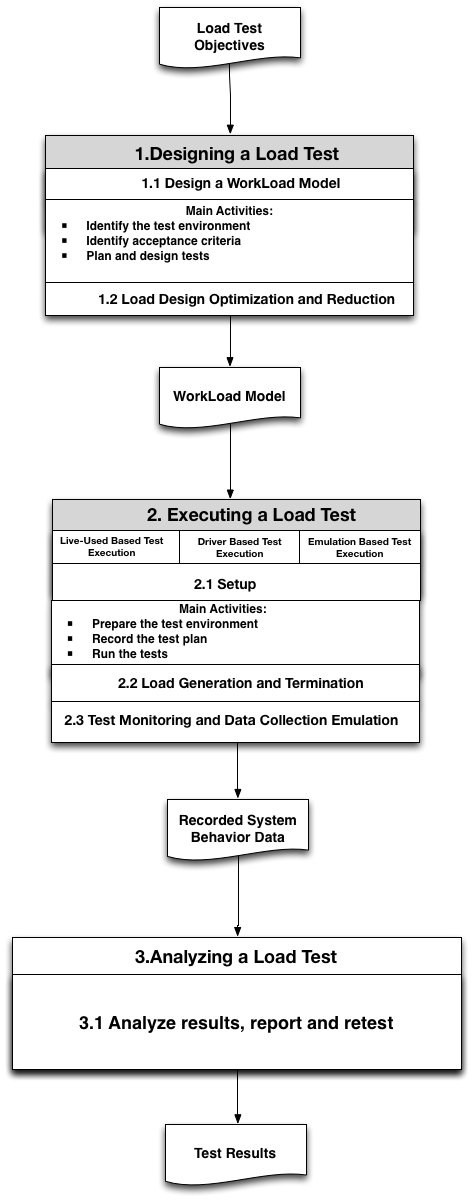
\includegraphics[width=0.5\textwidth]{./images/testprocess.png}
\caption{Load, Performance and Stress Test Process \cite{Jiang2010}\cite{Erinle2013}}
\label{fig:testprocess}
\end{figure}


The goal of the load design phase is to devise a load, which can uncover non-functional problems. Once the load is defined, the system under test executes the load and the system behavior under load is recorded. Load testing practitioners then analyze the system behavior to detect problems \cite{Jiang2010}. 

Once a proper load is designed, a load test is executed. The load test execution phase consists of the following three main aspects: (1) Setup, which includes system deployment and test execution setup; (2) Load Generation and Termination, which consists of generating the load; and (3) Test Monitoring and Data Collection, which includes recording the system behavior during execution\cite{Jiang2010}. 

The core activities in conducting an usual Load, Performance and Stress tests are \cite{Erinle2013}: 

\begin{itemize}
\item Identify the test environment: identify test and production environments and knowing the hardware, software, and network configurations helps derive an effective test plan and identify testing challenges from the outset.

\item Identify acceptance criteria: identify the response time, throughput, and resource utilization goals and constraints.

\item Plan and design tests:identify the test scenarios.In the context of testing, a scenario is a sequence of steps in an application. It can represent a use case or a business function such as searching a product catalog, adding an item to a shopping cart, or placing an order \cite{Corporation2007}. This task includes a description
of the speed, availability, data volume throughput rate, response
time, and recovery time of various functions, stress, and so on. This
serves as a basis for understanding the level of performance and
stress testing that may be required to each test scenario \cite{Lewis2005}.

\item Prepare the test environment: configure the test environment, tools, and resources necessary to conduct the planned test scenarios.

\item Record the test plan: record the planned test scenarios using a testing tool.

\item Run the tests: Once recorded, execute the test plans under light load and verify the correctness of the test scripts and output results.

\item Analyze results, report, and retest: examine the results of each successive run and identify areas of bottleneck that need addressing.  

\end{itemize}



\subsection{Automated Stress Test Tools}

Automated tools are needed to carry out serious load, stress, and performance testing. Sometimes, there is simply no practical way to provide reliable, repeatable performance tests without using some form of automation. The aim of any automated test tool is to simplify the testing process. Automated Test Tool  typically have the following components \cite{Molyneaux2009}:

\begin{itemize}
\item Scripting module: Enable recording of end-user activities in different middleware protocols;
\item Test management module: Allows the creation of test scenarios;
\item Load injectors: Generate the load with multiple workstations or servers;
\item Analysis module: Provides the ability to analyse the data collected by each test interation.
\end{itemize}

Apache JMeter is a free open source stress testing tool.  It has a large user base and offers lots of plugins to aid testing. JMeter is a desktop application designed to test and measure the performance and functional behavior of applications. The application it's purely Java-based and is highly extensible through a provided API (Application Programming Interface). JMeter works by acting as the client of a client/server application. JMeter allows multiple concurrent users to be simulated on the application \cite{Halili2008} \cite{Erinle2013}. 

JMeter has components organized  in a hierarchical manner. The Test Plan is the main component in a JMeter script. A typical test plan will consist of one or more Thread Groups, logic controllers, listeners, timers, assertions, and configuration elements:

\begin{itemize}
\item Thread Group: Test management module responsible to simulate the users used in a test. All elements of a test plan must be under a thread group.
\item Listeners: Analysis module responsible to provide access to the information gathered by JMeter about the test cases .
\item Samplers: Load injectors module responsible to send requests to a server, while Logical Controllers let you customize its logic.
\item Timers: allow JMeter to delay between each request.
\item Assertions: test if the application under test it is returning the correct results.
\item Configuration Elements: configure detais about the request protocol and test elements.
\end{itemize}


\subsection{Stress Test Results}

The system behavior recorded during the test execution phase needs to be analyzed to determine if there are any load-related functional or non-functional problems \cite{Jiang2010}. There can be many formats of system behavior like resource usage data or end-to-end response time, which is recorded as response time for each individual request. These types of data need to be processed before comparing against threshold values.A proper data summarization technique is needed to describe these many data instances into one number. Some researchers advocate that the 90-percentile response time is a better measurement than the average/medium response time, as the former accounts for most of the peaks, while eliminating the outliers \cite{Jiang2010}.

\section{Research Question 1:How is a proper stress designed?}

The design of a stress test depends intrinsically on the load model applied to the software under test. Based on the objectives, there are two general schools of thought for designing a proper load to achieve such objectives \cite{Afzal2009a}:

\begin{itemize}
\item Designing Realistic Loads (Workload Descriptive). 
\item Designing Fault-Inducing Loads ( Workload Generative).
\end{itemize}

In Designing Realistic Loads, the main goal of testing is to ensure that the system can function correctly once. Designing Fault-Inducing Loads  aims to design loads, which are likely to cause functional or non-functional problems \cite{Afzal2009a}.

Stress testing projects should start with the development of a model for user workload that an application receives. This should take into consideration various performance aspects of the application and the infrastructure that a given workload will impact. A workload is a key component of such a model \cite{Molyneaux2009}.

The term workload represents the size of the demand that will be imposed on the application under test in an execution. The metric  used for measure a workload is dependent on the application domain, such as the length of the video in a transcoding application for multimedia files or the size of the input files in a file compression application \cite{Feitelson2013} \cite{Molyneaux2009} \cite{Goncalves2014}. 

Workload is also defined by the load distribution between the identified transactions at a given time. Workload helps researchers study the system behavior identified in several load models. A workload model can be designed to verify the predictability, repeatability, and scalability of a system \cite{Feitelson2013} \cite{Molyneaux2009}.


Workload modeling is the attempt to create a simple and generic model that can then be used to generate synthetic workloads. The goal is typically to be able to create workloads that can be used in performance evaluation studies. Sometimes, the synthetic workload is supposed to be similar to those that occur in practice in real systems \cite{Feitelson2013} \cite{Molyneaux2009}.

There are two kinds of workload models: descriptive and generative. The main difference between the two is that descriptive models just try to mimic the phenomena observed in the workload, whereas generative models try to emulate the process that generated the workload in the first place \cite{DiLucca2006}. 

In descriptive models, one finds different levels of abstraction on the one hand and different levels of fidelity to the original data on the other hand. The most strictly faithful models try to mimic the data directly using the statistical distribution of the data. The most common strategy used in descriptive modeling is to create a statistical model of an observed workload (Fig. \ref{fig:descriptivemodel}). This model is applied to all the workload attributes, e.g., computation, memory usage, I/O behavior, communication, etc. \cite{DiLucca2006}. Fig. \ref{fig:descriptivemodel} shows a simplified workflow of a descriptive model. The workflow has six phases. In the first phase, the user uses the system in the production environment. In the second phase, the tester collects the user's data, such as logs, clicks, and preferences, from the system. The third phase consists in developing a model designed to emulate the user's behavior. The fourth phase is made up of the execution of the test, emulation of the user's behavior, and log gathering.



\begin{figure}[!ht]

\centering
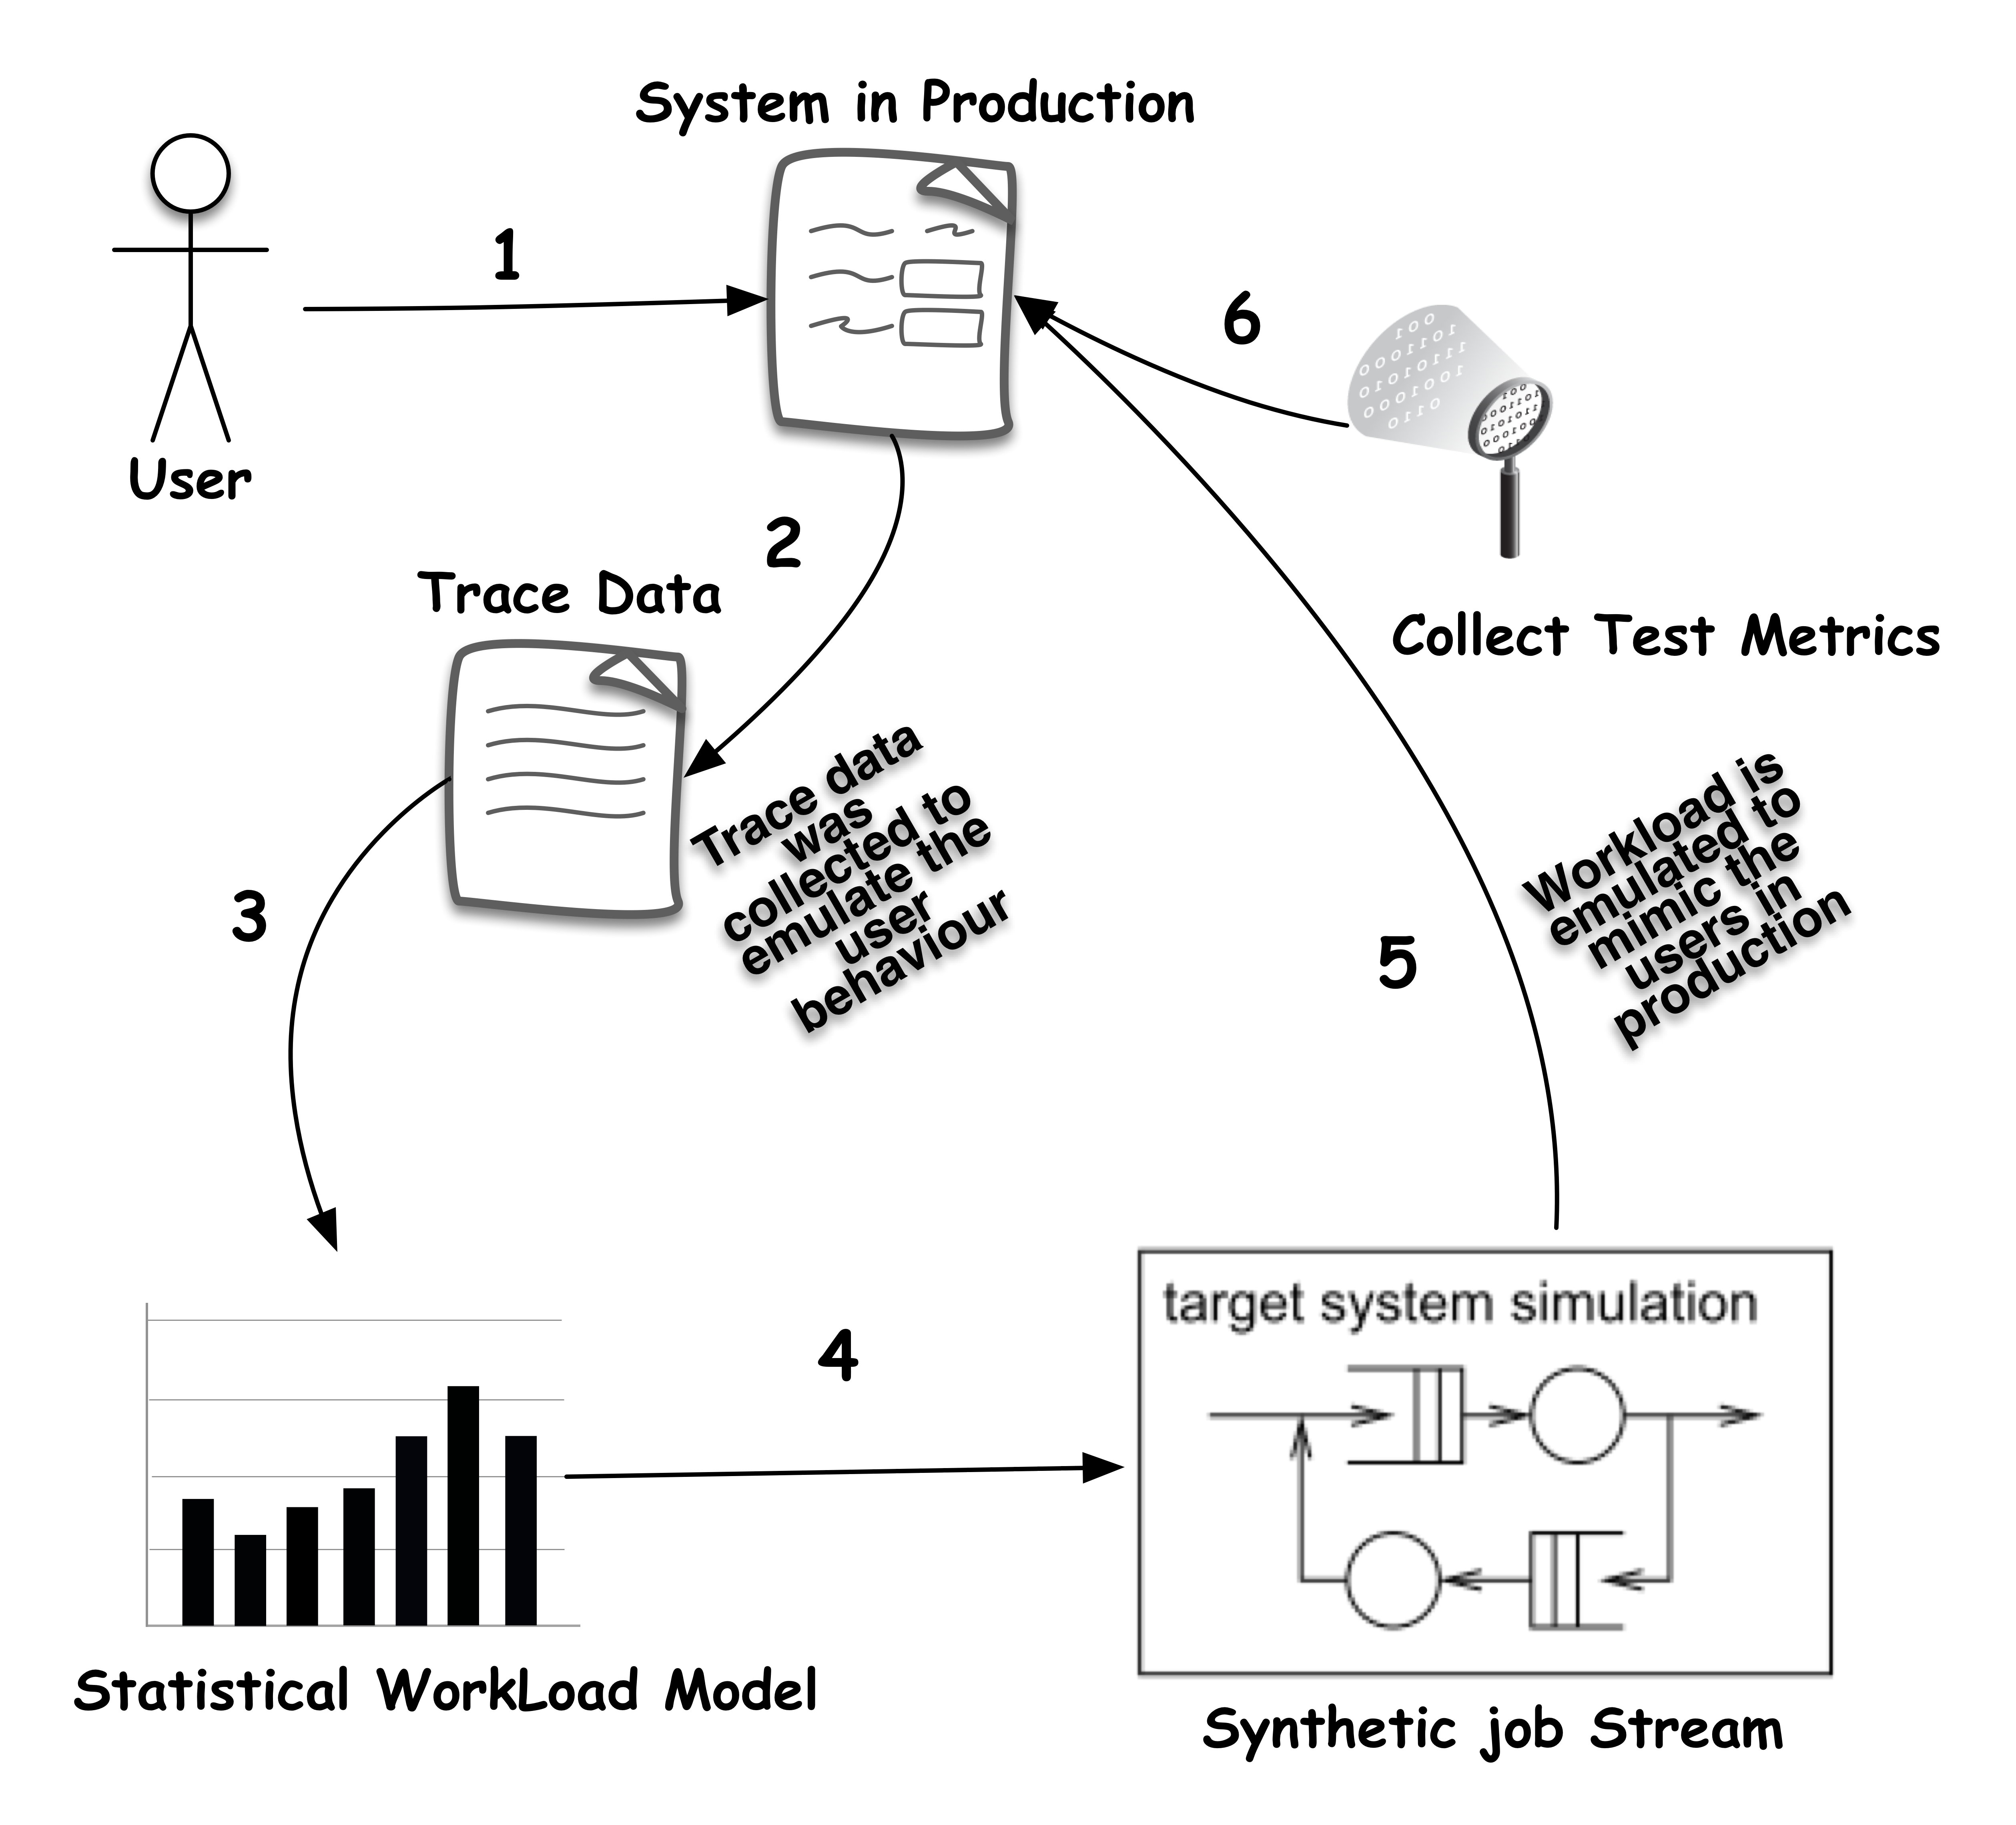
\includegraphics[width=0.8\textwidth]{./images/workloadmodel1300dpi.png}
\caption{Workload modeling based on statistical data \cite{DiLucca2006}}
\label{fig:descriptivemodel}
\end{figure}


Generative models are indirect in the sense that they do not model the statistical distributions. Instead, they describe how users will behave when they generate the workload. An important benefit of the generative approach is that it facilitates manipulations of the workload. It is often desirable to be able to change the workload conditions as part of the evaluation. Descriptive models do not offer any option regarding how to do so. With the generative models, however, we can modify the workload-generation process to fit the desired conditions \cite{DiLucca2006}. The difference between the workflows of the descriptive and the generative models is that user behavior is not collected from logs, but simulated from a model that can receive feedback from the test execution (Fig. \ref{fig:generativemodel}).


\begin{figure}[!ht]
\centering
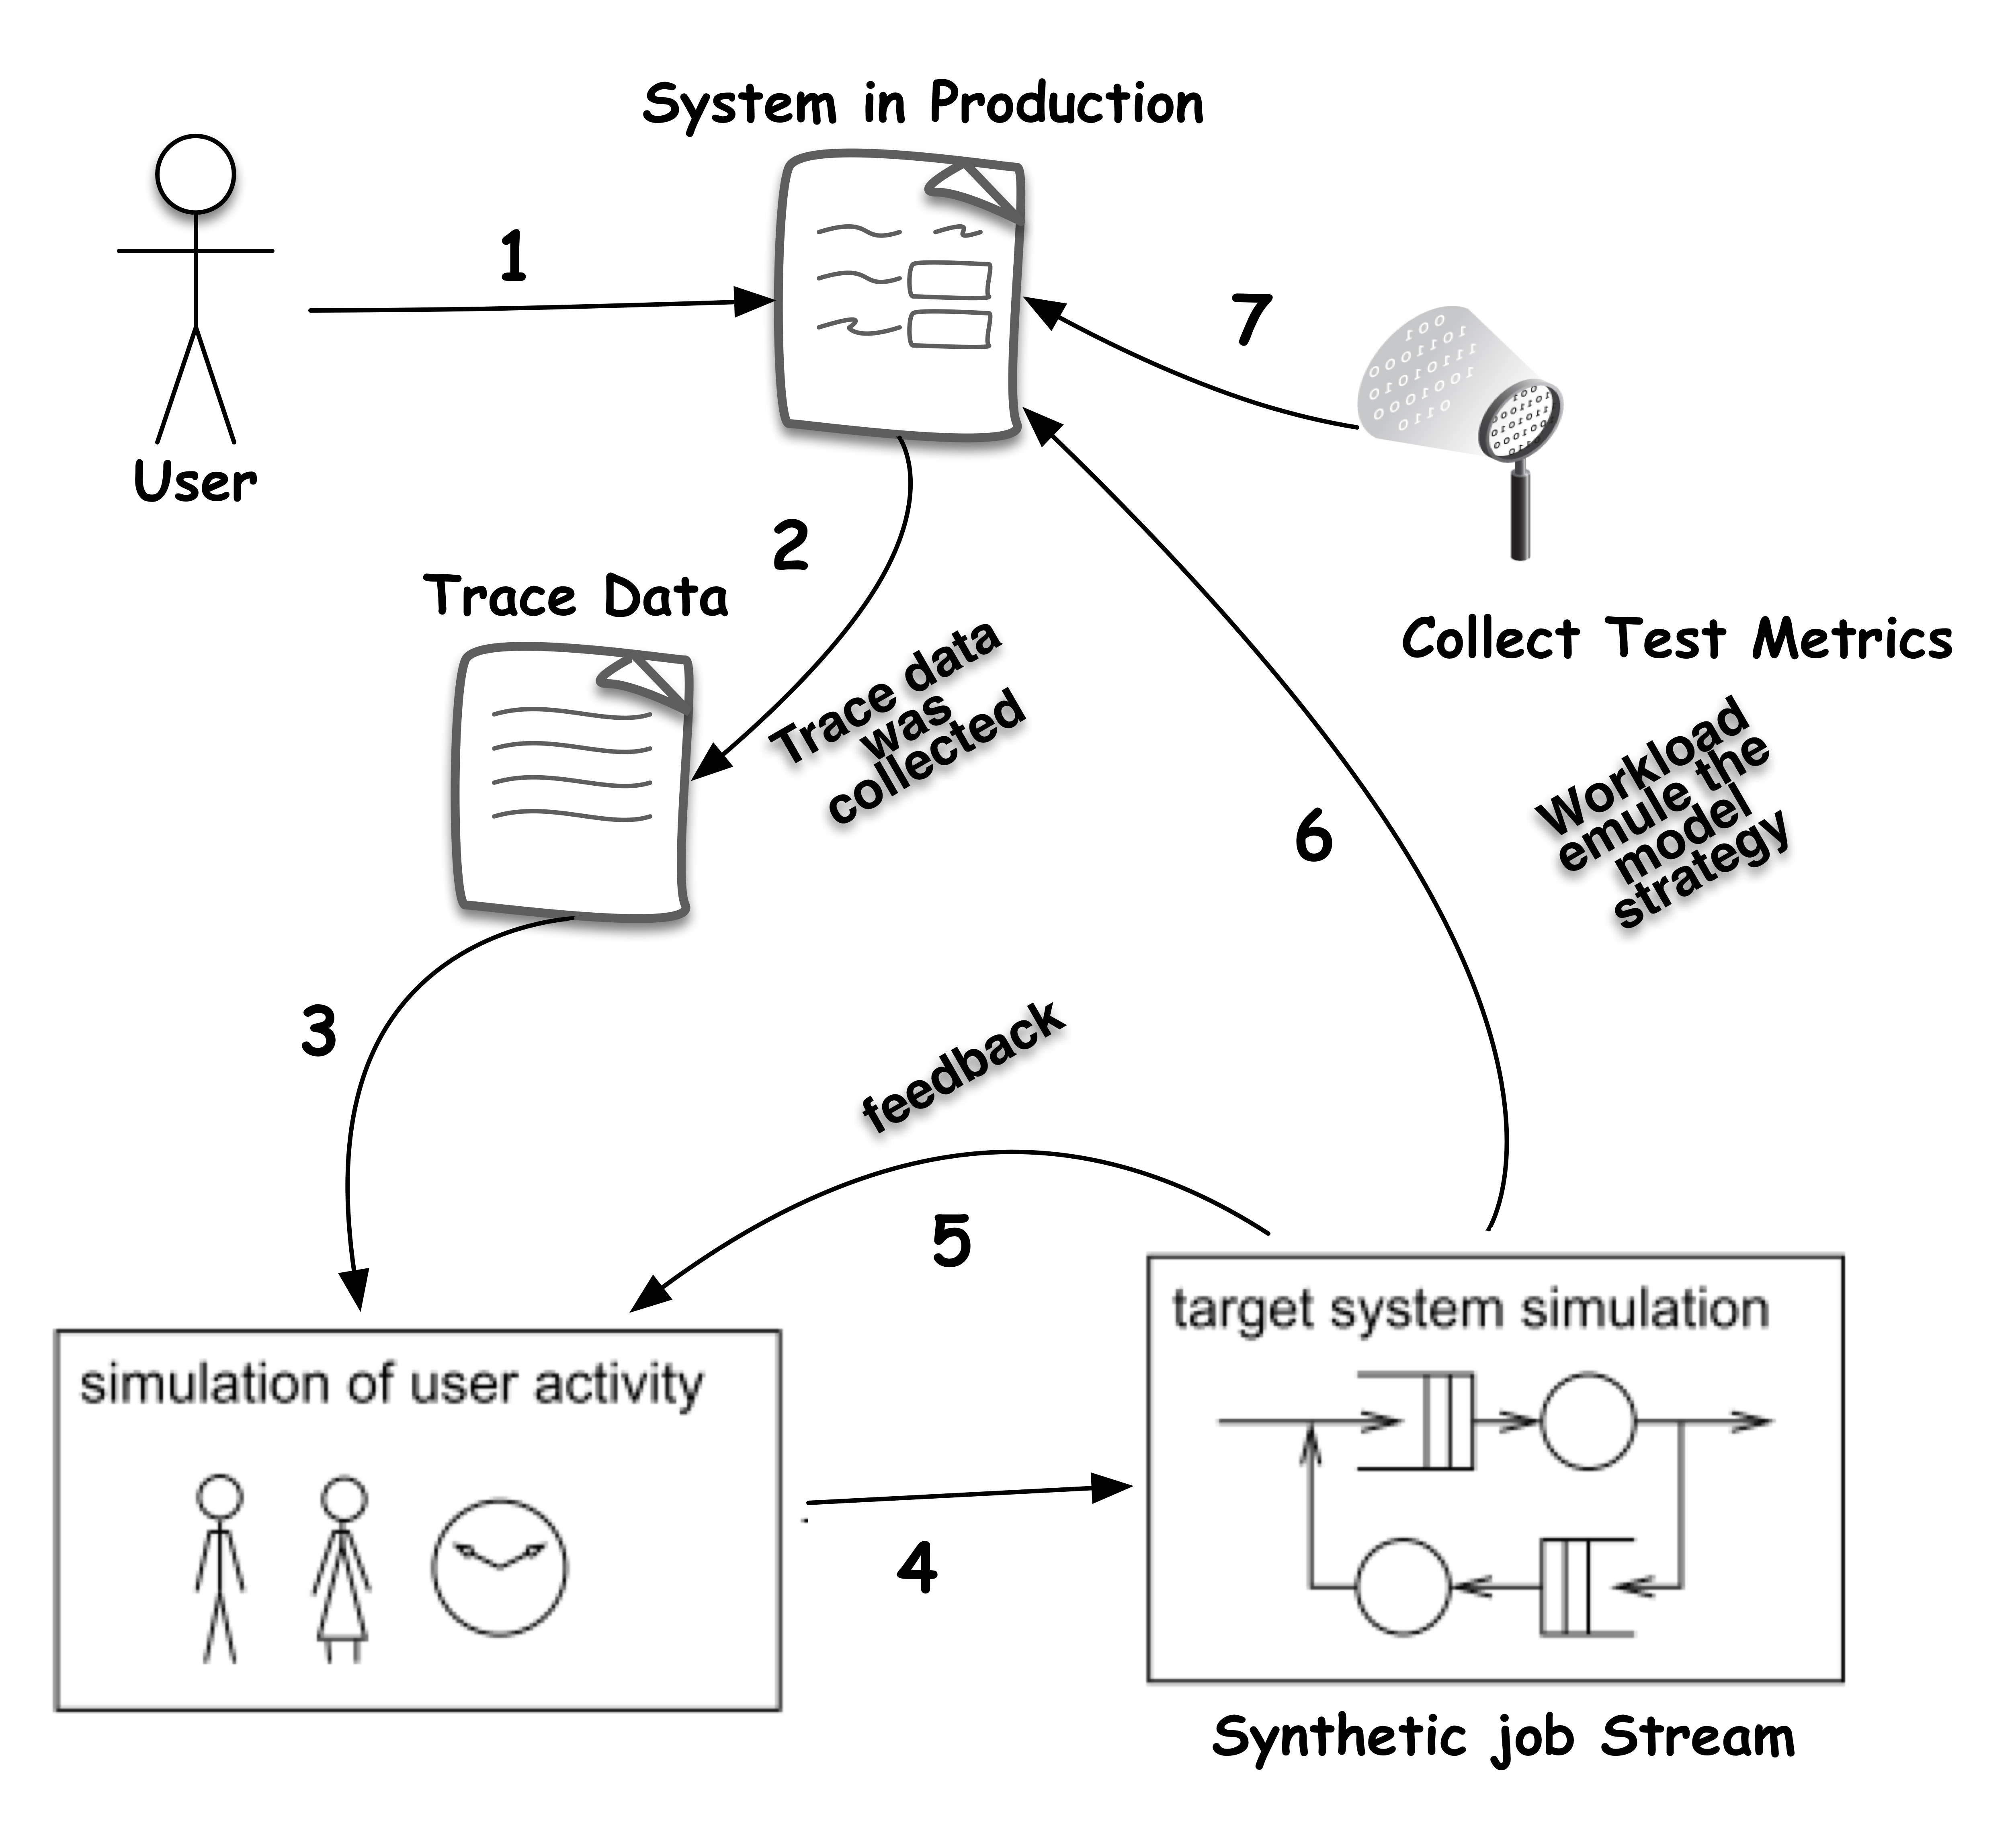
\includegraphics[width=0.8\textwidth]{./images/workloadmodel2300dpi.png}
\caption{Workload modeling based on the generative model \cite{DiLucca2006}}
\label{fig:generativemodel}

\end{figure}

Both load model have their advantages and disadvantages. In general, loads resulting from realistic-load based design techniques (Descriptive models) can be used to detect both functional and non-functional problems. However, the test durations are usually longer and the test analysis is more difficult. Loads resulting from fault-inducing load design techniques (Generative models) take less time to uncover potential functional and non-functional problems, the resulting loads usually only cover a small portion of the testing objectives \cite{Jiang2010}. The presented research work uses a generative model.


There are  several approaches to design generative or descriptive workloads:

\begin{itemize}
\item Model-based Stress testing: a usage model is proposed to simulate users’ behaviors.
\item Feedback-Directed Learning Software Testing:\cite{Luo2015} \cite{Wert2014}
\item Search-based Stress testing:
\end{itemize}

\subsection{Model-based Stress Testing}

Some research aproaches proposes models to simulate or  generate realistic loads. A User Community Modeling Language (UCML) is a set of symbols that can be used to create visual system usage models and depict associated parameters \cite{Wang2013}. The Fig. \ref{fig:ucml} shows a sample where all users realize a login into the application unde test. Once logged in, 40\% of the users navigates on the aplication, 30\%  of the users realizes downloads. 20\% of users realizes uploads and 10\% of users performs deletions.



\begin{figure}[!ht]
\centering
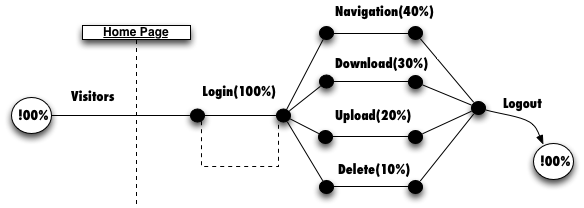
\includegraphics[width=1\textwidth]{./images/ucml.png}
\caption{User community modeling language \cite{Wang2013}}
\label{fig:ucml}

\end{figure}

Another technique to create workload models it is Stochastic Formcharts. Stochastic Formcharts are the combination of form oriented model and probability features. The Fig. \ref{fig:stform} shows a sample where all users have a probability of 100\% of realize a login into the application under test. Once logged in, users have a probability of 40\% of naviagte on the application and so on \cite{Draheim2006b}.


\begin{figure}[!ht]
\centering
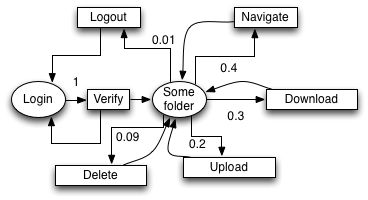
\includegraphics[width=1\textwidth]{./images/stochastic.png}
\caption{Stochastic Formcharts Example \cite{Draheim2006b} \cite{Wang2013}}
\label{fig:stform}
\end{figure}


\section{Research Question 2: How is a stress test executed and automated?}

The stress test execution phase consists of three phases:

\begin{itemize}
\item  Setup: which includes system deployment and test execution setup;
\item Load Generation and Termination: which consists of generating the load according to the configurations and terminating the load when the load test is completed;
\item Test Monitoring and Data Collection, which includes recording the system behavior.
\end{itemize}
 
 
There are three general approaches of load test executions:

\begin{itemize}
\item Live-User Based Executions: The test examines a system’s behavior when the system is simultaneously used by many users or execute a load test by employing a group of human testers. 
\item Driver Based Executions: The driver based execution approach automatically generate thousands or millions of concurrent requests for a long period of time using a software tool.
\item Emulation Based Executions: The emulation based load test execution approach performs the load testing on special platforms and doesn't require a fully functional system and conduct load testing.
\end{itemize}

There are three categories of load drivers: 



There are several tool to execution of Stress testing. In this tools, the procedure is semi-automated, whereas the execution of the tests itself is performed by a tool, the choice of scenarios to be executed as well as the decision to start new execution batteries are activities of the test designer or tester.

Open STA is an open source software developed in C++, and released under the GPL licence. OpenSTA provides a script language which permits to simulate the activity of a user. This language can describe HTTP/S scenario and all the test executions is managed in a graphical interface. The composition of the test is
very simple, allowing the tester choose scripts for a test and a remote computer that will execute each test.

\section{Research Question 3: What are the main problems found by stress tests?}

 Performance problems share common symptoms and many performance problems described in the literature are defined by a particular set of root causes. Fig. \ref{fig:symptoms}  shows the symptoms of known performance problems \cite{Wert2013a}. 



\begin{figure}[h]
\centering
\includegraphics[width=0.8\textwidth]{./images/symptoms.png}
\caption{Symptoms of know performance problems \cite{Wert2013a}. }
\label{fig:symptoms}
\end{figure}


There are several antipatterns that details features about  common performance problems. Antipatterns are conceptually similar to patterns in that they document recurring solutions to common design problems. They are known as
antipatterns because their use produces negative consequences.  Performance antipatterns document common performance mistakes made in software architectures or designs. These software Performance antipatterns have four primary uses: identifying problems,
focusing on the
right level of abstraction,
effectively communicating
their causes to others, and prescribing solutions \cite{brown1998antipatterns}. The table \ref{antipatterns} present some of the most common performance antipatterns.


% Please add the following required packages to your document preamble:
% \usepackage{multirow}
% \usepackage[table,xcdraw]{xcolor}
% If you use beamer only pass "xcolor=table" option, i.e. \documentclass[xcolor=table]{beamer}
\begin{table}[H]
\centering
\caption{Performance antipatterns}
\label{antipatterns}
\begin{tabular}{|l|l|}
\hline
\rowcolor[HTML]{C0C0C0} 
\multicolumn{1}{|c|}{\cellcolor[HTML]{C0C0C0}\textbf{antipattern}} & \multicolumn{1}{c|}{\cellcolor[HTML]{C0C0C0}\textbf{Derivations}} \\ \hline
Blob or The God Class &  \\ \hline
 & Concurrent processing Systems \\ \cline{2-2} 
 & Piper and Filter Architectures \\ \cline{2-2} 
\multirow{-3}{*}{Unbalanced-Processing} & Extensive Processing \\ \hline
Circuitous Treasure Hunt &  \\ \cline{1-1}
Empty Semi Trucks &  \\ \cline{1-1}
Tower of Babel &  \\ \cline{1-1}
One-Lane Bridge &  \\ \cline{1-1}
Excessive Dynamic Allocation &  \\ \cline{1-1}
Traffic Jam &  \\ \cline{1-1}
The Ramp  &  \\ \cline{1-1}
More is Less & \multirow{-10}{*}{} \\ \hline
\end{tabular}
\end{table}

Blob antipattern is known by various names, including the “god” class [8] and the “blob” [2]. Blob is an antipattern whose problem is on the excessive message traffic generated by a single class or component, a particular resource does the majority of the work in a software. The Blob antipattern occurs when a single class or component either performs all of the work of an application or holds all of the application’s data. Either manifestation results in excessive message traffic that can degrade performance \cite{Cortellessa2007} \cite{Smith2000}.

A project containing a “god” class is usually has a single, complex controller class that is surrounded by simple classes that serve only as data containers. These classes typically contain only accessor operations (operations to get() and set() the data) and perform little or no computation of their own \cite{Smith2000}.
The  Figures \ref{fig:godclass} and \ref{fig:godclass2} describes an hypotetical system with a BLOB problem:
The Fig. \ref{fig:godclass} presents a sample where the Blob class uses the features A,B,C,D,E,F and G of the hypotetical system; The Fig. \ref{fig:godclass2}  shows a static view where  a complex software entity instance, i.e. Sd, is connected to other software instances, e.g. Sa, Sb and Sc, through many dependencies \cite{Vetoio2011}\cite{Wert2013a}.




\begin{figure}[h]
\centering
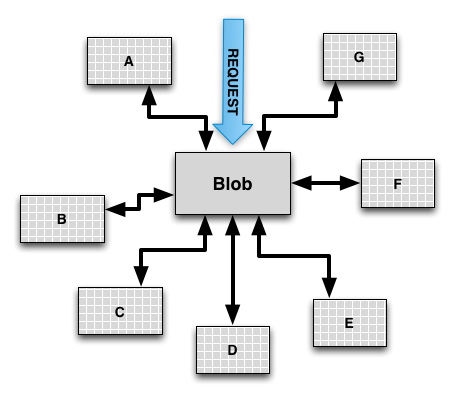
\includegraphics[width=0.8\textwidth]{./images/BLOB.png}
\caption{The God class\cite{Wert2013a}. }
\label{fig:godclass}
\end{figure}
\begin{figure}[h]
\centering
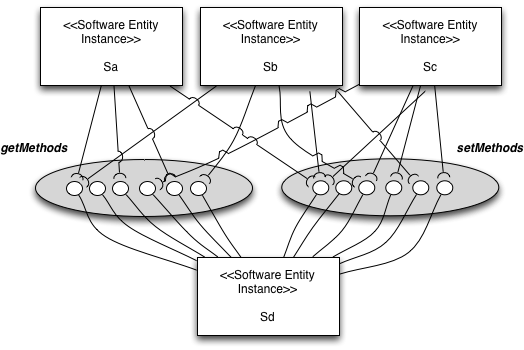
\includegraphics[width=0.8\textwidth]{./images/blob2.png}
\caption{The God class\cite{Vetoio2011}. }
\label{fig:godclass2}
\end{figure}

Unbalanced Processing it's characterises for one scenario where a specific class of requests generates a pattern of execution within the system that tends to overload a particular resource. In other words the overloaded resource will be executing a certain type of job very often, thus in practice damaging other classes
of jobs that will experience very long waiting times. Unbalanced Processing occurs in three different situations. The first case that cause unbalanced processing it is when processes cannot make effective use of available processors either because processors are dedicated to other tasks or because of single-threaded code. This manifestation has available processors and we need to ensure that the software is able to use them. Fig. \ref{fig:unbalanced}  shows a sample of the Unbalanced Processing. In The Fig. \ref{fig:unbalanced}, four tasks are performed. The task D it is waiting for the task C conclusion that are submmited to a heavy processing situation. 

The pipe and filter architectures  and extensive processing antipattern represents a manifestation of the unbalanced processing antipattern. The pipe and filter architectures occurs when the throughput of the overall system is determined by the slowest filter. The  Fig. \ref{fig:pipefilter} describes a software S with a Pipe and Filter Architectures problem: (a) Static View, there is a software entity instance, e.g. Sa, offering an operation (operation x) whose resource demand (computation = \$compOpx, storage = \$storOpx, bandwidth = \$bandOpx) is quite high; (b) Dynamic View, the operation opx is invoked in a service  and the throughput of the service (\$Th(S)) is lower than the required one. The extensive processing occurs when a process monopolizes a processor and prevents a set of other jobs to be executed until it finishes its computation. The Fig. \ref{fig:extpro} describes a software S with a Extensive Processing problem: (a) Static View, there is a software entity instance, e.g. Sa, offering two operations (operation x, operation y) whose resource demand is quite unbalanced, since opx has a high demand (computation = \$compOpx, storage = \$storOpx, bandwidth = \$bandOpx), whereas opy has a low demand (computation = \$compOpy, storage = \$storOpy, bandwidth = \$bandOpy); (b) Dynamic View, the operations opx and opy are alternatively invoked in a service and the response time of the service (\$RT(S)) is larger than the required one \cite{Vetoio2011}.

\begin{figure}[h]
\centering
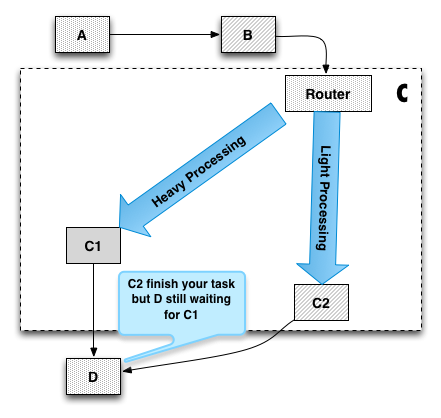
\includegraphics[width=0.5\textwidth]{./images/unbalanced.png}
\caption{Unbalanced Processing sample \cite{Wert2013a}. }
\label{fig:unbalanced}
\end{figure}


\begin{figure}[h]
\begin{minipage}{.5\textwidth}
\centering
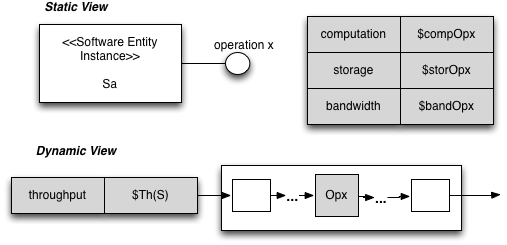
\includegraphics[width=1\textwidth]{./images/pipe2.png}
\caption{Pipe and Filter sample \cite{Vetoio2011}}
\label{fig:pipefilter}
\end{minipage}
\begin{minipage}{.5\textwidth}
\centering
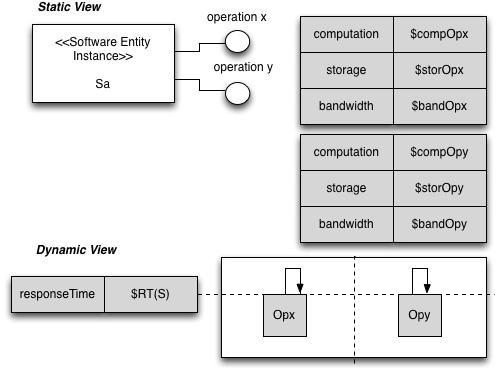
\includegraphics[width=1\textwidth]{./images/extpro.png}
\caption{Extensive Processing sample \cite{Vetoio2011}.}
\label{fig:extpro}
\end{minipage}
\end{figure}


Circuitous Treasure Hunt antipattern occurs when software retrieves data from a first componet, uses those results in a second component, retrieves data from the second component, and so on, until the last results are obtained \cite{Smith2002} \cite{Smith2003}. Circuitous Treasure Hunt 
are typical performance antipatterns that causes unnecessarily frequent database requests. The Circuitous Treasure Hunt antipattern is a result from a bad database schema or query design. A common Circuitous Treasure Hunt design creates a data dependency between single queries. For instance, a query requires the
result of a previous query as input. The longer the chain of
dependencies between individual queries the more the Circuitous
Treasure Hunt antipattern hurts performance \cite{Wert2014}. The Fig. \ref{fig:circuit}  shows a software S with a Circuitous Treasure Hunt problem: (a) Static View, there is a software entity instance e.g. Sa, retrieving information from the database; (b) Dynamic View, the software  S generates a large number of database calls by performing several queries up to the final operation \cite{Vetoio2011}.


\begin{figure}[h]
\centering
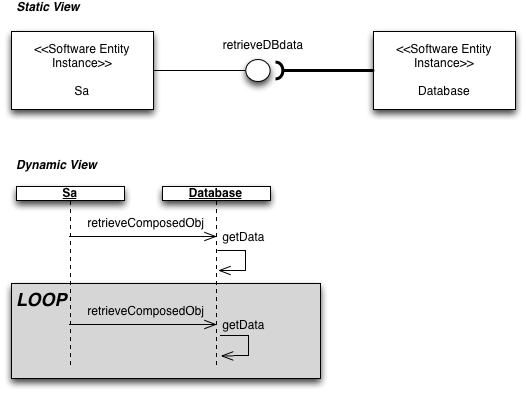
\includegraphics[width=1\textwidth]{./images/circuit.png}
\caption{Circuitous
Treasure Hunt sample \cite{Vetoio2011}}
\label{fig:circuit}
\end{figure}


\begin{figure}[h]
\centering
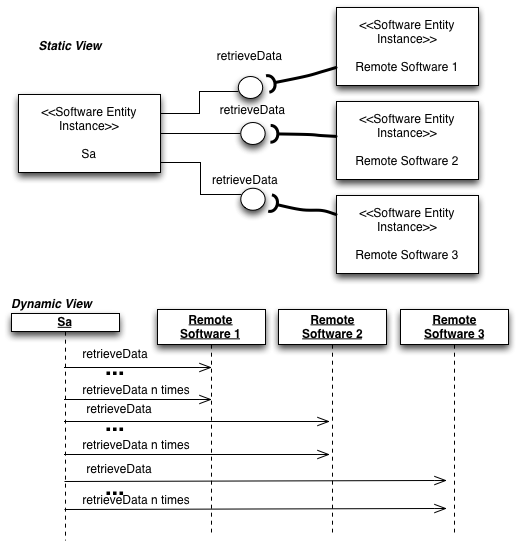
\includegraphics[width=0.8\textwidth]{./images/trucks.png}
\caption{Empty Semi Trucks sample \cite{Vetoio2011}.}
\label{fig:trucks}
\end{figure}

Empty Semi Trucks occurs when an excessive number of requests is required to perform a task. It may be due to inefficient use of available bandwidth, an inefficient interface, or both \cite{Arcelli2012}. There are a special case of Empty Semi Trucks that occurs  when many fields in a user interface must be retrieved from a
remote system. Fig. shows a software S with a Empty Semi Trucks problem: (a) Static View, there is a software entity instance, e.g. Sa, retrieving some information from several instances (Remote Software 1, . . . , Remote Software n); (b) Dynamic View, the software instance Sa generates an excessive message traffic by sending a big amount of messages with low sizes, much lower than the network bandwidth, hence the network link might have a low utilization value \cite{Vetoio2011}.

The Tower of Babel antipattern most often occurs when information is translated into an exchange format, such as XML, by the sending process then parsed and translated into an
internal format by the receiving process. When the translation and parsing is excessive, the system spends most
of its time doing this and relatively little doing real work \cite{Smith2003}. Fig. shows a system with a Tower of Babel problem: (a) Static View, there are some software entity instances, e.g. Sa, Sb, . . . , Sn; (b) Dynamic View, the software instances Sd performs many times the translation of format for communicating with other instances \cite{Vetoio2011}.

\begin{figure}[h]
\centering
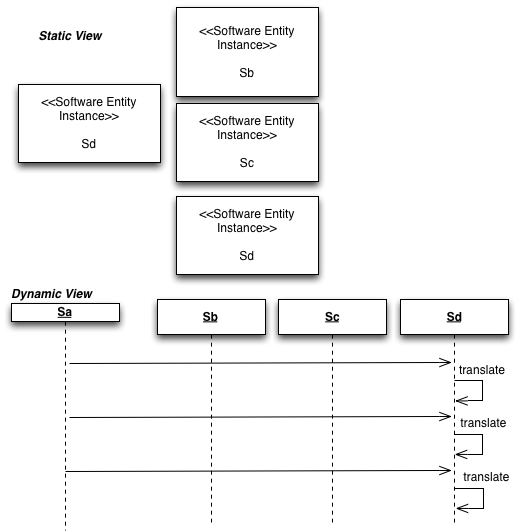
\includegraphics[width=0.6\textwidth]{./images/babel2.png}
\caption{Tower of Babel sample \cite{Vetoio2011}}
\label{fig:babel}
\end{figure}

\begin{figure}[h]
\centering
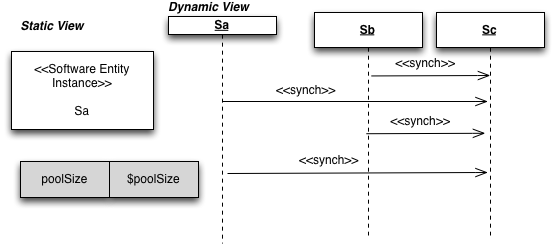
\includegraphics[width=1\textwidth]{./images/onelane.png}
\caption{One-Lane Bridge sample \cite{Vetoio2011}.}
\label{fig:onelane}

\end{figure}


One-Lane Bridge is a antipattern that occurs when one or a few processes execute concurrently using a shared resource and other processes are waiting for use the shared resource. It frequently occurs in applications that access a database. Here, a lock ensures that only one process may update the associated portion of the database at a time. This antipatterns is common when many concurrent threads or processes are waiting for the same shared resources. These can either be passive resources (like semaphores or mutexes) or active resources (like CPU or hard disk). In the first case, we have a typical One Lane Bridge whose critical resource needs to be identified. Figure 3.10 shows a system with a One-Lane Bridge problem: (a) Static View, there is a software entity instance with a capacity of managing \$poolSize threads; (b) Dynamic View, the software instance Sc receives an excessive number of synchronous calls in a service S and the predicted response time is higher than the required \cite{Vetoio2011}.


Using dynamic allocation, objects are created when they are first accessed and then destroyed when they are no longer needed. Excessive Dynamic Allocation, however, addresses frequent, unnecessary creation and destruction of objects of the same class. Dynamic allocation is expensive , an object created in memory must be allocated from the heap, and any initialization code for the object and the contained objects must be executed. When the object is no longer needed, necessary clean-up must be performed, and the reclaimed memory must be returned to the heap to avoid memory leaks \cite{Smith2002} \cite{Smith2003}.

\begin{figure}[H]
\begin{minipage}{.5\textwidth}
\centering
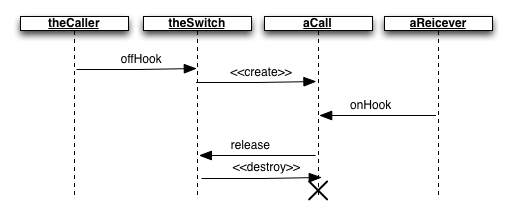
\includegraphics[width=1\textwidth]{./images/excessivedynamicallocation.png}
\caption{Excessive Dynamic Allocation.}
\label{fig:dynallocation}
\end{minipage}
\begin{minipage}{.5\textwidth}
\centering
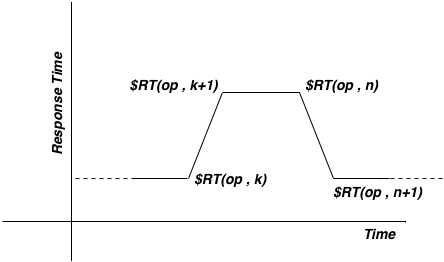
\includegraphics[width=1\textwidth]{./images/jam.png}
\caption{Traffic Jam Response Time \cite{Vetoio2011}.}
\label{fig:jam}
\end{minipage}
\end{figure}

The Fig. \ref{fig:dynallocation} shows a Excessive Dynamic Allocation sample. This example is drawn from a call (an offHook event), the switch creates a Call object to manage the call. When the call is completed, the Call object is destroyed. Constructing a single Call object it is not seem as excessive. A Call is a complex object that contains several other objects that must also be created. The Excessive Dynamic Allocation occurs when  a switch receive hundreds of thousands of offHook events. In a case like this, the overhead for dynamically allocating call objects adds substantial delays to the time needed to complete a call.

The Traffic Jam antipattern occurs if many concurrent threads or processes are waiting for the same  active resources (like CPU or hard disk). This antipatterns produces a large backlog in jobs waiting for service. The performance impact of the Traffic Jam is the transient behavior that produces wide variability in response time. Sometimes it is fine, but at other times, it is unacceptably long. Figure \ref{fig:jam} describes a software with a Traffic Jam problem, the monitored response time of the operation shows a wide variability in response time which persists long \cite{Vetoio2011}. 


\begin{figure}[H]
\begin{minipage}{.5\textwidth}
\centering
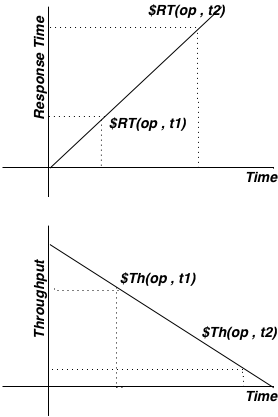
\includegraphics[width=0.5\textwidth]{./images/ramp.png}
\caption{The Ramp sample \cite{Vetoio2011}.}
\label{fig:ramp}
\end{minipage}
\begin{minipage}{.5\textwidth}
\centering
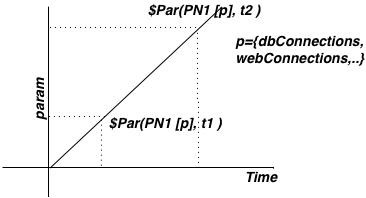
\includegraphics[width=1\textwidth]{./images/moreisless.png}
\caption{More is Less sample \cite{Vetoio2011}.}
\label{fig:moreisless}
\end{minipage}
\end{figure}

The Ramp it is a antipattern where the processing time increases as the system is used. The Ramp can arise in several different ways. Any situation in which the amount of processing required to satisfy a request increases over time will produce the behavior. With the Ramp antipattern, the memory consumption of the application is growing over time. The root cause is Specific Data Structures which are growing during operation or which are not properly disposed \cite{Wert2014} \cite{Smith2003}. Fig. \ref{fig:ramp} shows a system  with The Ramp problem:  (i) the monitored response time of the operation opx at time t1, i.e. \$RT(opx, t1), is much lower than the monitored response time of the operation opx at time t2, i.e. \$RT(opx, t2), with t1 < t2; (ii) the monitored throughput of the operation opx at time t1, i.e. \$Th(opx, t1), is much larger than the monitored throughput of the operation opx at time t2, i.e. \$Th(opx, t2), with t1 < t2. 

More is less occurs when a system spends more time "thrashing” than accomplishing real work because there are too many processes relative to available resources. More is Less are presented when it is running too many programs overtime. This antipattern causes too much system paging and systems spend all their time servicing page faults rather than processing requests. In distributed systems, there are more causes.They include: creating too many database connections and  allowing too many internet connection. Fig. \ref{fig:moreisless} describes a system  with a More Is Less problem: There is a processing node PN1 and the monitored runtime parameters (e.g. database connections, etc.) at time t1, i.e. \$Par(PN1[p], t1), are much larger than the same parameters at time t2, i.e. \$Par(PN1[p], t2), with t1 < t2. 







\chapter{Search-Based Stress Testing}


The goal of this Chapter is to describe Search-Based Testing, define recurring solutions in search-based testing

\section{Introduction}

Search-based software engineering (SBSE) is the application of optimization techniques in solving software engineering problems [1,2]. The applicability of optimization techniques in solving software engineering problems is suitable as these problems frequently encounter competing constraints and require near optimal solutions \cite{Afzal2009a} \cite{Harman2015}. 


Search Based Software Testing (SBST) is the sub-area of Search Based Software Engineering concerned with software testing. Search-based software testing is the application of metaheuristic search techniques to generate software tests. SBSE uses computational search techniques to tackle software engineering problems, typified by large complex search spaces. SBSE derives test inputs for a software system with the goal of improving various criteria. The test adequacy criterion is transformed into a fitness function and a set of solutions in the search space are evaluated with respect to the fitness function using a metaheuristic search technique \cite{Afzal2009a} \cite{Aleti2016} \cite{Harman2015}.

Stress search-based testing is a application of SBST where the main goal it is to find test scenarios that produce execution times that exceed the timing constraints specified. If a temporal error is found, the test was successful \cite{Sullivan}.

\section{Search-Based Testing}

Search-Based Testing is the process of automatically
generating test according to a test adequacy criterion,encoded as a fitness function, using search-based optimization algorithms, which are guided by a fitness function. The role of the fitness function is to capture a test objective that, when achieved, makes a contribution to the desired test adequacy criterion \cite{Harman2010}. 

Search–Based Testing uses metaheuristic algorithms to
automate the generation of test inputs that meet a test
adequacy criterion. Many algorithms have been considered in the past, including Simulated Annealing, Parallel Evolutionary Algorithms \cite{Alba2008},Evolution Strategies, Estimation of Distribution Algorithms , Scatter Search , Particle Swarm Optimization , Tabu Search and the Alternating Variable Method. An advantage of meta-heuristic algorithms is that they
are widely applicable to problems that are infeasible for analytic approaches. All one has to do is come up with a representation for candidate solutions and an objective function to evaluate those solution \cite{Baars2011}. 

The application of metaheuristic search techniques to test case generation is a possibility which offers much benefits. Metaheuristic search techniques are high-level frameworks which utilise heuristics in order to find solutions to combinatorial problems at a reasonable computational cost. Such a problem may have been classified as NP-complete or NP-hard, or be a problem for which a polynomial time algorithm is known to exist but is not practical \cite{McMinn2004}.

One of the most popular search techniques used in SBST belong to the family of Evolutionary Algorithms in what is known as Evolutionary Testing. Evolutionary Algorithms represent a class of adaptive search techniques based on natural genetics and Darwin’s theory of evolution. They are characterized by an iterative procedure that works in parallel on a number of potential solutions to a problem. Figure \ref{fig:evocycle}  shows the cycle
of an Evolutionary Algorithm when used in the context of
Evolutionary Testing \cite{Baars2011}.

\begin{figure}[h]
\centering
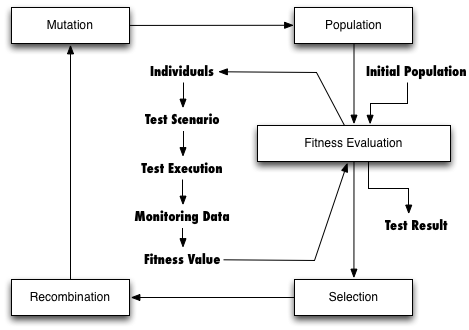
\includegraphics[width=1\textwidth]{./images/evolutionary.png}
\caption{Evolutionary Algorithm Search Based Test Cycle\cite{Baars2011}. }
\label{fig:evocycle}
\end{figure}

First, a population of possible solutions to a problem
is created, usually at random. Starting with randomly
generated individuals results in a spread of solutions ranging in fitness because they are scattered around the search–space. Next, each individual in the population is evaluated by calculating its fitness via a fitness function. The principle idea of an Evolutionary Algorithm is that fit individuals survive over time and form even fitter individuals in future
generations. Selected individuals are then recombined
via a crossover operator. After crossover, the resulting offspring individuals may be subjected to a mutation operator. The algorithm iterates until a global optimum is reached or another stopping condition is fulfilled \cite{Baars2011}. 

The fitness evaluation is the most
time consuming task of SBST. However, for time consuming functional testing of complex industrial systems, minimizing
the number of generated individuals may also be highly desirable. This might be done using an assumption about
the "potential" of individuals in order to predict which individuals are likely to contribute to any future improvement.
This prediction could be achieved by using information about similar individuals that have been executed in earlier generations.



\section{Non-functional Search-Based Testing}

SBST has made many achievements, and demonstrated its wide applicability and increasing uptake. Nevertheless, there are pressing open problems and challenges that need more attention like to extend SBST to test non-functional properties, a topic that remains relatively under-explored, compared to structural testing. There are many kinds of non-functional search based tests  \cite{Afzal2009a}:

\begin{itemize}
\item Execution time: The application of evolutionary algorithms to find the best and worst case execution times (BCET, WCET).
\item Quality of service: uses metaheuristic search techniques to search violations of service level agreements (SLAs).
\item Security: apply a variety of metaheuristic search techniques  to detect security vulnerabilities like detecting buffer overflows.
\item Usability: concerned with construction of covering array which is a combinatorial object.
\item Safety: Safety testing is an important component of the testing strategy of safety critical systems where the systems are required to meet safety constraints.
\end{itemize}

A variety of metaheuristic search techniques are found to be applicable for non-functional testing including simulated annealing, tabu search, genetic algorithms, ant colony methods, grammatical evolution, genetic programming and swarm intelligence methods. The Fig. \ref{fig:metabykind} shows a comparison between the range of metaheuristcs and the type of non-functional search based test.The Data comes from Afzal et al. \cite{Afzal2009a}. Afzal's work adds to some of the latest research in this area (\cite{Garousi2006} \cite{Garousi2010} \cite{DiAlesio2013} \cite{DiAlesio2014} \cite{Alesio2015} \cite{Gois2016}). 


\begin{figure}[h]
\centering
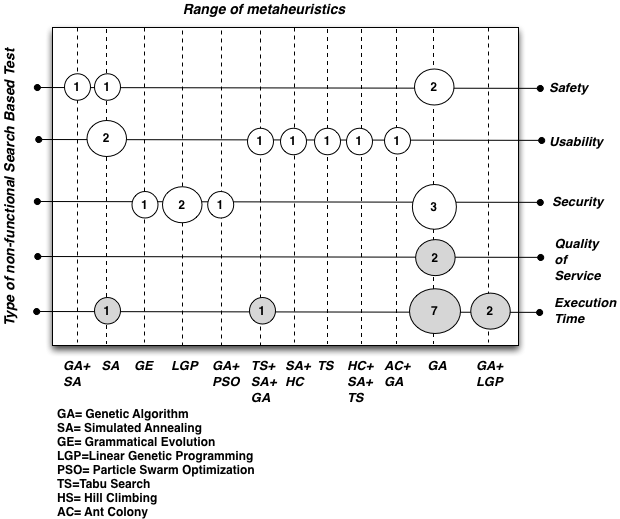
\includegraphics[width=1\textwidth]{./images/metaheuristics.png}
\caption{Range of metaheuristics by Type of non-functional Search Based Test\cite{Afzal2009a}. }
\label{fig:metabykind}
\end{figure}




\section{Search-Based Stress Testing}

The search for the longest execution time is regarded as a discontinuous, nonlinear, optimization problem, with the input domain of the system under test as a search space \cite{Sullivan}.  The application of SBST algorithms to  stress tests involves finding the best- and worst-case execution times (B/WCET) to determine whether timing constraints are fulfilled \cite{Afzal2009a}. 

There are two measurement units normally associated with the fitness function in stress test: processor cycles and execution time. The processor cycle approach describes a fitness function in terms of processor cycles. The execution time approach involves executing the application under test and measuring the execution time \cite{Afzal2009a} \cite{tracey2000search}.

Processor cycles measurement is deterministic in the sense that it is independent of system load and results in the same execution times for the same set of input parameters. However, such a measurement is dependent on the compiler and optimizer used, therefore, the processor cycles differ for each platform. Execution time measurement is a non deterministic approach, there is no guarantee to get the same results for the same test inputs \cite{Afzal2009a}.  However, stress testing where testers have no access to the production environment should be measured by the execution time measurement \cite{Molyneaux2009} \cite{Afzal2009a}.

Table \ref{tab:comparison}  shows a comparison between the research studies on load, performance, and stress tests presented by Afzal et al. \cite{Afzal2009a}. Afzal's work adds to some of the latest research in this area (\cite{Garousi2006} \cite{Garousi2010} \cite{DiAlesio2013} \cite{DiAlesio2014} \cite{Alesio2015} \cite{Gois2016} ). The columns represent the type of tool used (prototype or functional tool), and the rows represent the metaheuristic approach used by each research study (genetic algorithm, Tabu search, simulated annealing, or a customized algorithm). The table also sorts the research studies by the type of fitness function used (execution time or processor cycles). 


\begin{table}[h]
\centering
\caption{Distribution of the research studies over the range of applied metaheuristics}
\label{tab:comparison}
\begin{tabular}{p{2.2cm}|p{2.8cm}|p{2.8cm}|p{2.8cm}|}
\cline{2-4}
                                                                & \multicolumn{2}{c|}{\textbf{Prototypes}}            & \textbf{Functional Tool} \\ \cline{2-4} 
                                                                & \begin{minipage}{0.2\textwidth}\footnotesize Execution Time  \end{minipage}          & \begin{minipage}{0.2\textwidth}\footnotesize Processor Cycles \end{minipage}        & \begin{minipage}{0.2\textwidth}\footnotesize Execution Time \end{minipage}           \\ \cline{2-4} 
%\setlength{\extrarowheight}{20pt}
\begin{tabular}[c]{@{}l@{}}\begin{minipage}{0.1\textwidth}\scriptsize GA + SA  \\ + Tabu \\ Search \end{minipage}\end{tabular}  & \cellcolor[HTML]{FFFFFF} & \cellcolor[HTML]{FFFFFF} & \cellcolor[HTML]{FFFFFF} \begin{minipage}{0.2\textwidth} \tiny    Gois et al. 2016 \cite{Gois2016}  \end{minipage}  \\[2ex] \cline{2-4} 
\begin{minipage}{0.1\textwidth}\scriptsize GA \end{minipage}                                                              & \cellcolor[HTML]{FFFFFF} \begin{minipage}{0.12\textwidth}   \tiny \textnormal{ \\  Alander et al.,1998 \cite{Alander} \\ Wegener et al., 1996 and 1997 \cite{Wegener1997}\cite{J.WegenerK.GrimmM.GrochtmannH.Sthamer1996} \\  Sullivan et al., 1998 \cite{Sullivan} \\ Briand et al., 2005 \cite{Briand2005} \\ Canfora et al., 2005 \cite{Canfora}  \\ }\end{minipage} & \cellcolor[HTML]{FFFFFF} \begin{minipage}{0.12\textwidth} \tiny \textrm{  \\ Wegener and Grochtmann, 1998 \cite{Wegener1998} \\  Mueller et al., 1998 \cite{Mueller1998} \\ Puschner et al. \cite{Puschner1998} \\ Wegener et al., 2000 \cite{Stations} \\ Gro et al., 2000 \cite{Gross2000}  \\ }\end{minipage}& \cellcolor[HTML]{FFFFFF} \begin{minipage}{0.12\textwidth}   \tiny \textnormal{ \\  Di Penta, 2007 \cite{Penta2007} \\ Garoussi, 2006 \cite{Garousi2006} \\ Garousi, 2008 \cite{Garousi2008} \\ Garousi, 2010 \cite{Garousi2010} \\ } \end{minipage} \\[2ex] \cline{2-4} 
\begin{minipage}{0.1\textwidth}\scriptsize Simulated \\ Annealing \\ (SA) \end{minipage}                                                             & \cellcolor[HTML]{FFFFFF} & \cellcolor[HTML]{FFFFFF} & \cellcolor[HTML]{FFFFFF} \begin{minipage}{0.12\textwidth}   \tiny  Tracey, 1998 \cite{Tracey1998} \end{minipage} \\[2ex] \cline{2-4}
\begin{minipage}{0.1\textwidth}\scriptsize  Constraint \\ Programming \end{minipage}                                                             & \cellcolor[HTML]{FFFFFF} & \cellcolor[HTML]{FFFFFF} & \cellcolor[HTML]{FFFFFF} \begin{minipage}{0.12\textwidth}   \tiny  Alesio, 2014 \cite{DiAlesio2014} \\ Alesio, 2013 \cite{DiAlesio2013}  \end{minipage} \\[2ex] \cline{2-4} 
\begin{minipage}{0.1\textwidth}\scriptsize  GA +\\ Constraint \\ Programming \end{minipage}                                                             & \cellcolor[HTML]{FFFFFF} & \cellcolor[HTML]{FFFFFF} & \cellcolor[HTML]{FFFFFF} \begin{minipage}{0.12\textwidth}   \tiny  Alesio, 2015 \cite{Alesio2015} \end{minipage} \\[2ex] \cline{2-4} 
\setlength{\extrarowheight}{20pt}
\begin{tabular}[c]{@{}l@{}}
\begin{minipage}{0.1\textwidth}\scriptsize Customized \\ Algorithm \end{minipage}\end{tabular} & \cellcolor[HTML]{FFFFFF} & \cellcolor[HTML]{FFFFFF}  \begin{minipage}{0.12\textwidth}   \tiny  \textnormal{   \raggedleft Pohlheim, 1999 \cite{Pohlheim2005}  } \end{minipage} & \cellcolor[HTML]{FFFFFF} \\[4ex] \cline{2-4}
\end{tabular}
\end{table}

The studies can be grouped into two main groups:

\begin{itemize}
\item Search-Based Stress Tesing on Safety-critical systems.
\item Search-Based Stress Testing on Industrial systems.
\end{itemize}


\subsection{Search-Based Stress Tesing on Safety-critical systems}

Domains such as avionics, automotive and aerospace feature safety-critical systems, whose failure could result in catastrophic consequences.  The importance
of software in such systems is permanently increasing due to the need of a higher system
flexibility. For this reason, software components of these systems are usually subject to safety certification. In this context, software safety certification has to take into account performance requirements specifying constraints on how the system should react to its environment, and how it should execute on its hardware platform \cite{DiAlesio2013}.

Usually, embedded computer systems have to fulfil real-time requirements. A faultless function of the systems does not depend only on their logical correctness but also on their temporal correctness. Dynamic aspects like the duration of computations, the memory actually needed during program execution, orthe synchronisation of parallel processes are of major importance for the correct function of real-time systems  \cite{J.WegenerK.GrimmM.GrochtmannH.Sthamer1996} .

The concurrent nature of embedded software makes  the order of external events triggering the systems tasks is often unpredictable. Such increasing software complexity
renders performance analysis and testing increasingly
challenging. This aspect is reflected by the fact that most existing testing approaches target system functionality rather than performance \cite{DiAlesio2013}.

Reactive real-time systems must react to external events within time constraints. Triggered tasks must execute within deadlines. Shousha develops a methodology for the derivation of test cases that aims at maximizing the chance of critical deadline misses \cite{shousha2003performance}. 

The main goal of Search-Based Stress testing of Safety-critical systems it is finding a combination of inputs that causes the system to delay task completion to the greast extent possible \cite{shousha2003performance}. The followed approaches uses metaheuristics to discover the worst-case execution times. 

Wegener et al. \cite{Wegener1997} used genetic algorithms(GA) to search for input situations that produce very long or very short execution times. The fitness function used was the execution time of an individual measured in micro seconds \cite{Wegener1997}. Alander et al. \cite{Alander} performed experiments in a simulator environment to measure response time extremes of protection relay software using genetic algorithms. The fitness function used was the response time of the tested software. The results showed that GA generated more input cases with longer response times \cite{Alander}. 

Wegener and Grochtmann performed a  experimentation
to compare GA with random testing. The fitness function used was duration of execution measured in processor cycles.  The results showed that, with a large number of input parameters, GA obtained more extreme execution times with less or equal testing effort than random testing \cite{J.WegenerK.GrimmM.GrochtmannH.Sthamer1996} \cite{Wegener1998}.


Gro et. al. \cite{Gross2000} presented a prediction model  which can be used to predict evolutionary testability. The research confirmed that there is a relationship between the complexity of a test object and the ability of a search algorithm to produce input parameters according to B/WCET \cite{Gross2000}. 

Briand et al. \cite{Briand2005} used GA to find the sequence of arrival times of events for aperiodic tasks, which will cause the greatest delays in the execution of the target task. A prototype tool named real-time test tool (RTTT) was developed to facilitate the execution of runs of genetic algorithm. Two case studies were conducted and results illustrated that RTTT was a useful tool to stress a system under test \cite{Briand2005}.


Pohlheim and Wegener used an extension of genetic algorithms with multiple sub-populations, each using a different search strategy. The duration of execution measured in processor cycles was taken as the fitness
function. The GA found longer execution times for all the given modules in comparison with systematic testing\cite{Pohlheim2005}.

Garousi presented a stress test methodology aimed at increasing chances of discovering faults related to distributed traffic in distributed systems. The technique uses as input a specified UML 2.0 model of a system, augmented with timing information.The results indicate that the technique is significantly more effective at detecting distributed traffic-related faults when compared to standard test cases based on an operational profile \cite{Garousi2006}.

Alesio, Nejati and Briand describe a approach based
on Constraint Programming (CP) to automate the generation of test cases that reveal, or are likely to, task deadline misses. They evaluate it through a comparison with a state-of-the-art approach based on Genetic Algorithms (GA). In particular, wthe study compares CP and GA in five case studies for efficiency, effectiveness, and scalability. The experimental results show that, on the largest and more complex case studies, CP performs significantly better than GA. The research proposes a tool-supported, efficient and effective approach based on CP to generate stress test cases that maximize the likelihood of task deadline misses \cite{DiAlesio2013}.

Alesio describe stress test case generation as a search problem over the space of task arrival times. The research search for worst case scenarios maximizing deadline misses where each scenario characterizes a test case. The paper combine two strategies, GA and Constraint Programming (CP). The results show that, in comparison with GA and CP in isolation, GA+CP achieves nearly the same effectiveness as CP and the same efficiency and solution diversity as GA, thus combining the advantages of the two strategies. Alesio concludes that a combined GA+CP approach to stress testing is more likely to scale to large and complex systems \cite{Alesio2015}.

\subsection{Search-Based Stress Testing on Industrial systems} 

Usually, the application of Search-Based Stress Testing on non safety-critical systems deals with the generation of test cases that causes Service Level Agreements violations.


Tracey et al. \cite{Tracey1998} used simulated annealing (SA) to test four
simple programs. The results of the research presented that the use of SA was more effective with larger parameter space. The authors highlighted the need of a detailed comparison of various optimization techniques to explore WCET and BCET of the of the system under test \cite{Tracey1998}.

Di Penta et al. \cite{Penta2007} used GA to create test data that violated QoS constraints causing SLA violations. The generated test data included combinations of inputs. The approach was applied to two case studies. The first case study was an audio processing workflow. The second case study, a service producing charts, applied the black-box approach with fitness calculated only on the basis of how close solutions violate QoS constraint. The genome representation is presented in Fig \ref{fig:dipenta}. The representation models a wsdl request to a webservice.

\begin{figure}[h]
\centering
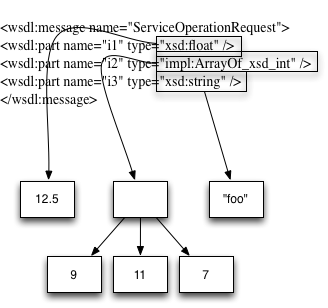
\includegraphics[width=0.6\textwidth]{./images/dipenta.png}
\caption{Genome representation \cite{Penta2007}. }
\label{fig:dipenta}
\end{figure}



In case of audio workflow, the GA outperformed random search. For the second case study, use of black-box approach successfully violated the response time constraint, showing the violation of QoS constraints for a real service available on the Internet \cite{Penta2007}.


Gois et al. proposes an hybrid metaheuristic approach using genetic algorithms, simulated annealing, and tabu search algorithms to perform stress testing. A tool named IAdapter, a JMeter plugin used for performing search-based stress tests, was developed. Two experiments were performed to validate the solution. In the first experiment, the signed-rank Wilcoxon non- parametrical procedure was used for comparing the results. The significant level adopted was 0.05. The procedure showed that there was a significant improvement in the results with the Hybrid Metaheuristic approach.
In the second experiment, the whole process of stress and performance tests, which took 3 days and about 1800 executions, was carried out without the need for monitoring by a test designer. The tool automatically selected the next scenarios to be run up to the limit of six generations previously established \cite{Gois2016}. 


\chapter{Metaheuristics}


Following the complexity of the problem, it may be solved by an exact method or an
approximate method. Exact methods obtain optimal solutions and guarantee
their optimality. Approximate (or heuristic) methods generate high quality
solutions in a reasonable time for practical use, but there is no guarantee of finding a global optimal solution \cite{Talbi2013}.


\begin{figure}[h]
\centering
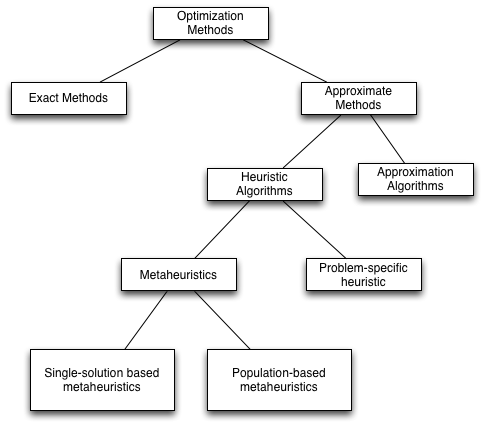
\includegraphics[width=1\textwidth]{./images/optimization.png}
\caption{Classical optimization methods \cite{Talbi2013}. }
\label{fig:optimization}
\end{figure}


In the computer science, the term metaheuristic is accepted for general techniques which are not specific to a particular problem. A metaheuristic is formally defined as an iterative generation process which guides a subordinate heuristic by combining intelligently different concepts for exploring and exploiting the search space \cite{raidl2010metaheuristic}. 

Metaheuristics are strategies that guide the search process to efficiently explore the search space in order to find optimal solutions. Metaheuristic algorithms are approximate and usually non-deterministic and sometimes incorporate mechanisms to avoid getting trapped in confined areas of the search space. There are different ways to classify and describe metaheuristic algorithm \cite{Blum2003}:

\begin{itemize}
\item Nature-inspired vs. non-nature inspired. There are nature-inspired algorithms, like Genetic Algorithms and Ant Algorithms, and non nature-inspired ones such as Tabu Search and Iterated Local Search. 

\item Population-based vs. single point search. Algorithms working on single solutions are called trajectory methods, like Tabu Search, Iterated Local Search and Variable Neighborhood Search. They all share the property of describing a trajectory in the search space during the search process. Population-based metaheuristics perform search processes which describe the evolution of a set of points in the search space.

\item One vs. various neighborhood structures. Most metaheuristic algorithms work on one single neighborhood structure. In other words, the fitness landscape topology does not change in the course of the algorithm. Other metaheuristics, such as Variable Neighborhood Search (VNS), use a set of neighborhood structures which gives the possibility to diversify the search by swapping between different fitness
landscapes.
\end{itemize}

\section{Single-Solution Based Metaheuristics}

While solving optimization problems, single-solution based metaheuristics
 improve a single solution. They could be viewed as "walks" through neighborhoods or search trajectories through the search space of the problem at hand.
 
 \begin{figure}[h]
\centering
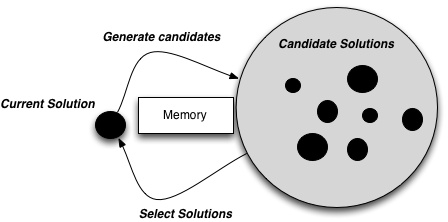
\includegraphics[width=1\textwidth]{./images/singlebased.png}
\caption{ Main principles of single-based metaheuristics.}
\label{fig:singlebased}
\end{figure}


\subsection{Neighborhood}

The definition of Neighborhood is a required common step for the design of any Single-Solution metaheuristic (S-metaheuristic). The neighborhood structure it is a important piece in the performance of an S-metaheuristic. If the neighborhood structure is not adequate to the problem,
any S-metaheuristic will fail to solve the problem. The neighborhood function N is a mapping: $ N : S \rightarrow N\textsuperscript{2} $ that assigns to each solution s of \textit{S} a set of solutions \textit{N(s)}$\subset$ S \cite{Talbi2013}.

The neighborhood definition depends  representation associated with the problem. For permutation-based representations, a usual neighborhood is based on the swap operator that consists in swapping the location of two elements $s_i$ and $s_j$ of the permutation \cite{Talbi2013}.


\begin{figure}[h]
\centering
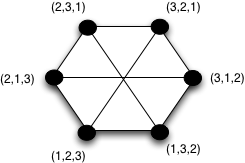
\includegraphics[width=0.6\textwidth]{./images/neighborhood.png}
\caption{ An example of neighborhood for a permutation \cite{Talbi2013}.}
\label{fig:sperneighborhood}
\end{figure}



Single-Solution Based Metaheuristics methods are characterized by a trajectory in the search space. Two common S-metaheuristics methods are Simulated Annealing and Tabu Search.


\subsection{Simulated Annealing}

Simulated Annealing (SA) is a randomized algorithm that tries to avoid being trapped in local optimum solution by assigning probabilities to deteriorating moves. The SA procedure is inspired from the annealing process of solids. SA is based on a physical
process in metallurgy discipline or solid matter physics. Annealing is the process of obtaining low energy states of a solid in heat treatment \cite{Jaziri2008}. 

The algorithmic framework of SA is described in Alg. \ref{sa}.  The algorithm starts by generating an initial solution in function \textit{GenerateInitialSolution()}. The initial temperature value is determined in function \textit{SetInitialTemperature()} such that the probability for an uphill move is quite high at the start of the algorithm. At each iteration a solution $\mbox{s}_1$ is randomly chosen in function \textit{PickNeighborAtRandom(N(s))}. If \textit{$\mbox{s}_1$} is better than \textit{s}, then \textit{$\mbox{s}_1$} is accepted as new current solution. Else, if the move from \textit{s} to \textit{$\mbox{s}_1$} is an uphill move, \textit{$\mbox{s}_1$}  is accepted with a probability which is a function of a temperature parameter \textit{Tk} and \textit{s} \cite{raidl2010metaheuristic}. 

\begin{algorithm}[h]
  \caption{Simulated Annealing Algorithm}\label{sa}
  \begin{algorithmic}[1]
    
    \State $s\gets GenerateInitialSolution()$
    \State $k\gets 0 $
    \State $Tk\gets SetInitialTemperature()$
    \While{termination conditions not met }
    \State $\mbox{s}_1\gets PickNeighborAtRandom(N (s))$
    \If{$(f(\mbox{s}_1)<f(s))$}
    \State $s\gets\mbox{s}_1$
    \Else $\;$ Accept $\mbox{s}_1$ as new solution with probability p($\mbox{s}_1|$Tk,s) 
    \EndIf
    \State $K\gets K+1$
    \State $Tk\gets AdaptTemperature()$
    \EndWhile
      
  \end{algorithmic}
\end{algorithm}

\subsection{Tabu Search}

Tabu Search (TS) is a metaheuristic that guides a local heuristic search procedure to explore the solution space beyond local optimal and search with short term memory to avoid cycles. Tabu Search uses a  tabu list to keep track of the last  moves, and don’t allow going back to these \cite{Glover1986}.

The basic idea of TS is the explicit use of search history, both to escape
from local minima and to implement a strategy for exploring the search space.
A basic TS algorithm uses short term memory in the form of socalled
tabu lists to escape from local minima and to avoid cycles \cite{Tobergte2013}.

The algorithmic framework of Tabu Search is described in Alg. \ref{tsa}.  The algorithm starts by generating an initial solution in function \textit{GenerateInitialSolution()} and the tabu lists are initialized as empty lists in function \textit{InitializeTabuLists($\mbox{TL}_1$,...,$\mbox{TL}_r$)}. For performing a move, the algorithm first determines those solutions from the neighborhood \textit{N(s)} of the current solution \textit{s} that contain solution features currently to be found in the tabu lists. They are excluded from the neighborhood, resulting in a restricted set of neighbors \textit{$\mbox{N}_a(s)$}. At each iteration the best solution \textit{$\mbox{s}_1$} from \textit{$\mbox{N}_a(s)$} is chosen as the new current solution. Furthermore, in procedure \textit{UpdateTabuLists($\mbox{TL}_1$,...,$\mbox{TL}_r$,s,$\mbox{s}_1$)} the corresponding features of this solution are added to the tabu lists.


\begin{algorithm}[h]
  \caption{Tabu Search Algorithm}\label{tsa}
  \begin{algorithmic}[2]
    
    \State $s\gets GenerateInitialSolution()$
    \State InitializeTabuLists($\mbox{TL}_1$,...,$\mbox{TL}_r$)
    \While{termination conditions not met }
    \State $\mbox{N}_a(s)\gets$ $\{\mbox{s}_1 \in N(s) |\mbox{s}_1$ does not violate a tabu condition, or it satisfies at least one aspiration condition $\}$ 
    \State $\mbox{s}_1\gets argmin\{f(\mbox{s}_2)|\mbox{s}_2 \in \mbox{N}_a(s) \}$
    \State UpdateTabuLists($\mbox{TL}_1$,...,$\mbox{TL}_r$,s,$\mbox{s}_1$)
    \State $s\gets \mbox{s}_1$
    \EndWhile
      
  \end{algorithmic}
\end{algorithm}

\section{Population-based metaheuristics}

Population-based metaheuristics (P-metaheuristics) could be viewed as an iterative improvement in a population of solutions. First, the population is initialized. Then, a new population of solutions is generated. Finally, this new population is integrated into the current one using some selection procedures. The search process is stopped when a stopping criterion is satisfied. Algorithms such as Genetic algorithms (GA), scatter search (SS), estimation of distribution algorithms (EDAs), particle swarm optimization (PSO), bee colony (BC), and artificial immune systems (AISs) belong to this class of metaheuristics \cite{talbi2009metaheuristics}. 

\subsection{Genetic Algorithms}

Genetic Algorithms could be a mean of solving complex optimization problems that are often NP Hard. GAs are based on concepts adopted from genetic and evolutionary theories. GAs are comprised of several components \cite{hong2000simultaneously} \cite{shousha2003performance} :

\begin{itemize}
\item a representation of the solution, refered as the chromossome;
\item fitness of each chromossome, refered as objective function;
\item the genetic operations of crossover and mutation which generate new offspring. 
\end{itemize}


Algorithm \ref{gna} shows the basic structure of GA algorithms. In this algorithm, P denotes the population of individuals. A population of offspring is generated by the application of recombination and mutation operators and the individuals for the next population are selected from the union of the old population and the offspring population \cite{raidl2010metaheuristic}.


\begin{algorithm}[h]
  \caption{Genetic Algorithm}\label{gna}
  \begin{algorithmic}[3]
    
    \State $s\gets GenerateInitialSolution()$
    \State Evaluate(P)
    \While{termination conditions not met }
    \State $\mbox{P}_1\gets$ $Recombine(P)$
    \State $\mbox{P}_2\gets$ $Mutate(\mbox{P}_1)$ 
    \State $Evaluate(\mbox{P}_2)$
    \State $P\gets Select(\mbox{P}_2,P)$
    \EndWhile
      
  \end{algorithmic}
\end{algorithm}

\section{Hybrid  Metaheuristics}

However, in recent years it has become evident that the concentration on a sole metaheuristic is rather restrictive. A skilled combination of a metaheuristic with other optimization techniques, a so called hybrid metaheuristic, can provide a more efficient behavior
and a higher flexibility when dealing with real-world and large-scale problems \cite{Talbi2012}.

A combination of one metaheuristic with components from other metaheuristics is called a hybrid metaheuristic. The concept of hybrid metaheuristics has been commonly accepted only in recent years, even if the idea of combining different metaheuristic strategies and algorithms dates back to the 1980s. Today, we can observe a generalized common agreement on the advantage of combining components from different search techniques and the tendency of designing hybrid techniques is widespread in the fields of operations research and artificial intelligence \cite{raidl2010metaheuristic}. 


There are two main categories of metaheuristic combinations: collaborative combinations and integrative combinations. These are presented in Fig. \ref{fig:metaheuristc} \cite{Raidl2006}.

\begin{figure}[h]
\centering
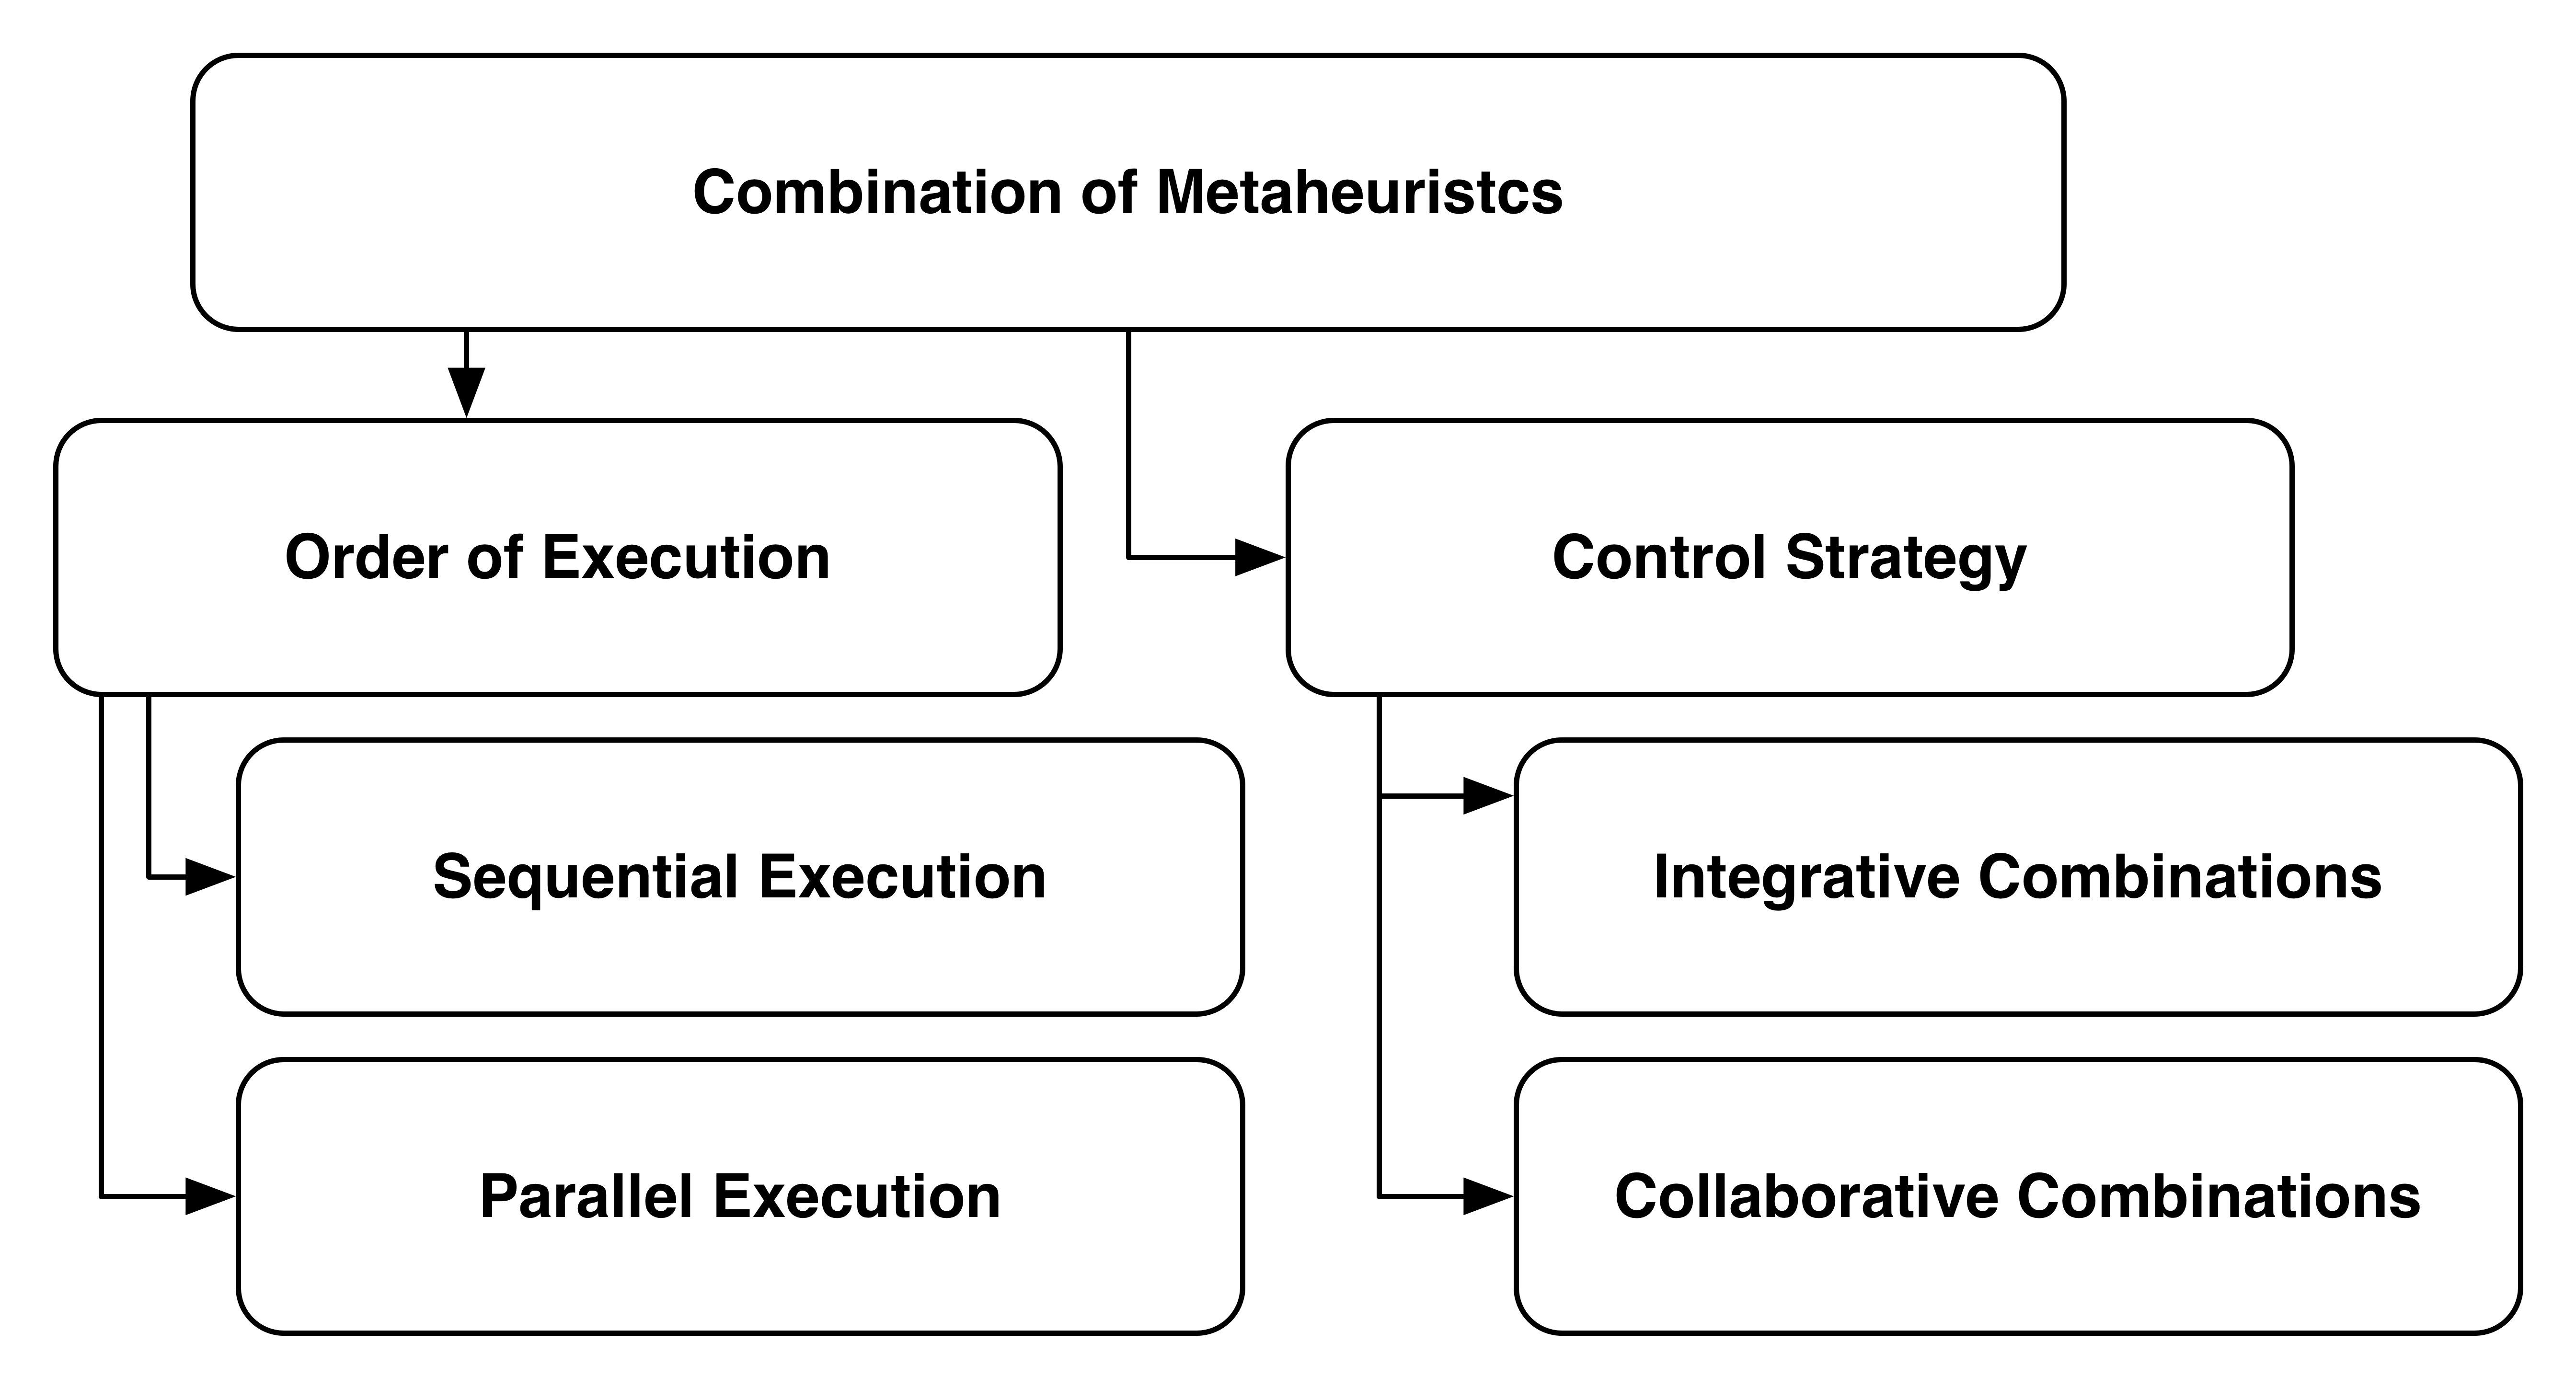
\includegraphics[width=1\textwidth]{./images/metaheuristc2.png}
\caption{Categories of metaheuristc combinations \cite{Puchinger2005} }
\label{fig:metaheuristc}
\end{figure}

Collaborative combinations use an approach where the algorithms exchange information, but are not part of each other. In this approach, algorithms may be executed sequentially or in parallel. 

One of the most popular ways of metaheuristic hybridization consists in the use of trajectory methods inside population-based methods. Population-based methods are better in identifying promising areas in the search space from which trajectory methods can quickly reach good local optima. Therefore, metaheuristic hybrids that can effectively combine the strengths of both population-based methods and trajectory methods are often very successful \cite{raidl2010metaheuristic}.


The work uses a type of collaborative combination with sequential execution with two trajectory methods (Tabu Search and Simulated Annealing) and Genetic Algorithms.



\chapter{Q-Learning}




\section{Reinforcement Learning}

Reinforcement learning (RL) refers to both a learning problem and a subfield of machine
learning. As a learning problem, it refers to learning to control a system so as to maximize
some numerical value which represents a long-term objective. A typical setting where
reinforcement learning operates is shown in Figure 1: A controller receives the controlled
system’s state and a reward associated with the last state transition. It then calculates an
action which is sent back to the system.


\begin{figure}
\centering
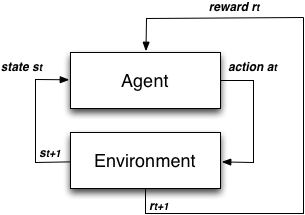
\includegraphics[width=0.7\textwidth]{./images/agentenv.png}
\caption{Example of a simple MDP with three states and two actions}
\label{fig:agentenv}
\end{figure}


The basis idea of Reinforcement learning  is simply to capture the most important aspects of the real problem facing a learning agent interacting with its environment to achieve a goal \cite{Sutton2012}. Reinforcement learning is learning what to do—how to map situations to actions—so as to maximize a numerical reward signal. The learner need to discover which actions yield the most reward by trying them \cite{Sutton2012}.

In Reinforcement Learning, an agent wanders in an unknown environment and tries to maximize its long term return by performing actions and receiving rewards. The challenge is to understand how a current action will affect future rewards. A good way to model this task is with Markov Decision Processes (MDP), which have become the dominant approach in Reinforcement Learning.

In Reinforcement Learging, all agents act in two phases: Exploration vs Explotation. In Exploration phase, the agents tries discover better action selections to improve its knowledge. In Explotation phase, the agents tries to maximize its reward, based on what its already know.

One of the challenges that arise in reinforcement learning is the trade-off between exploration and exploitation. To obtain a lot of reward, a reinforcement learning
agent must prefer actions that it has tried in the past and found to be effective in producing reward.
But to discover such actions, it has to try actions that it has not selected before. The agent has to exploit what it already knows in order to obtain reward, but it also has to explore in order to make better action selections in the future.


\subsection{Markov decision processes}

Markov decision processes (MDPs) provide a mathematical framework for modeling decision making. A countable MDP is defined as a triplet $M=(\chi,A,P_{0})$ \cite{Szepesvari2010}. where $\chi$ is a set of states, A is a set of actions. The transition probability kernel $P_{0}$ assigns to each state-action pair $(x, a) \in \chi x A $


The six main elements of a MDP are:(1) state of the system, (2) actions, (3) transition probabilities, (4) transition rewards, (5) a policy, and (6) a performance metric \cite{Sutton2012}.

\begin{figure}
\centering
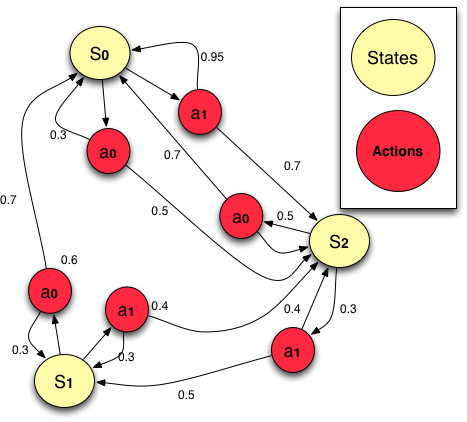
\includegraphics[width=0.7\textwidth]{./images/mdp1.png}
\caption{Example of a simple MDP with three states and two actions}
\label{fig:mdp}
\end{figure}


The state of a system is a parameter or a set of parameters that can be used to describe a system. For example the geographical coordinates of a robot can be used to
describe its state. A system whose state changes with time is called a dynamic system. Then it is not hard to see why a moving robot produces a dynamic system.

Actions are the controls allowed for an agent. Transition Probability denotes the probability of going from state i to state j under the influence of action a in one step. If an MDP has 3 states and 2 actions, there are 9 transition probabilities per action. Usually, the system receives an immediate reward ,which could be positive or negative, when it transitions from one state to another

A policy defines the learning agent’s way of behaving at a given time. Roughly speaking, a policy is a mapping from perceived states of the environment
to actions to be taken when in those states. It corresponds to what in
psychology would be called a set of stimulus–response rules or associations.  Policys mapping from states to actions.

Performance Metric: Associated with any given policy, there exists a so-called performance
metric — with which the performance of the policy is judged. Our goal is to select the policy
that has the best performance metric. 

\subsection{Types of Control Learnings}


Fig. shows the basic types of control learning problems. The first criterion that the space of problems is split upon is whether the learner can actively influence the observations.In case she can, then we talk about interactive learning, otherwise one is facing a non-interactive learning problem.

Interactive learning is potentially easier since the learner has the additional option to influence the distribution of the sample. However, the goal of
learning is usually different in the two cases, making these problems incomparable in general.

In the case of non-interactive learning, the natural goal is to find a good policy given the observations.
A common situation is when the sample is fixed. For example, the sample can be the result of some experimentation with some physical system that happened before learning started. 

Consider now interactive learning. One possibility is that learning happens while interacting
with a real system in a closed-loop fashion. A reasonable goal then is to optimize online performance,
making the learning problem an instance of online learning. Online performance
can be measured in different ways. A natural measure is to use the sum of rewards incurred
during learning. 




\section{Q-Learning}

Q-learning is a model-free reinforcement learning technique. Q-learning, it is a multiagent learning algorithm that learns equilibrium policies in Markov games, just as Q-learning learns to optimal policies in Markov decision processes \cite{Greenwald2003}. 

Q-learning and related algorithms tries to learn the optimal policy from its history of interaction with the environment. A history of an agent is a sequence of state-action-rewards.Where $s_{n}$ it is a state, $a_{n}$ it is an action and $r_{n}$ is a reward:

\begin{equation}
<s_{0},a_{0},r_{1},s_{1},a_{1},r_{2},s_{2},a_{2},r_{3},s_{3},a_{3},r_{4},s_{4}....>,
\end{equation}


In Q-Learning, the system's objective is to learn a control policy $\pi = \sum_{n=0}^{\infty} \gamma\textsuperscript{n}  r_{t}+n $, where $\pi$  is the discounted cumulative reward, $\gamma$ is the discount rate ($01$) and $r_{t}$ is the reward reiceved after execution an action at time t.

\section{GridWorld Example}

The GridWorld problem is an example of using reinforcement learning with Q-Learning. In this example, extracted from \url{http://www.cs.ubc.ca/~poole/demos/rl/q.html}, there are four rewarding states (apart from the walls), one worth +10 (at position (9,8); 9 across and 8 down), one worth +3 (at position (8,3)), one worth -5 (at position (4,5)) and one -10 (at position (4,8)). In each if these states the agent gets the reward when it carries out an action in that state.

The numbers in the squares shows the Q-values of the square for each action. The blue arrows show the optimal action based on the current value function.

\begin{figure}
\centering
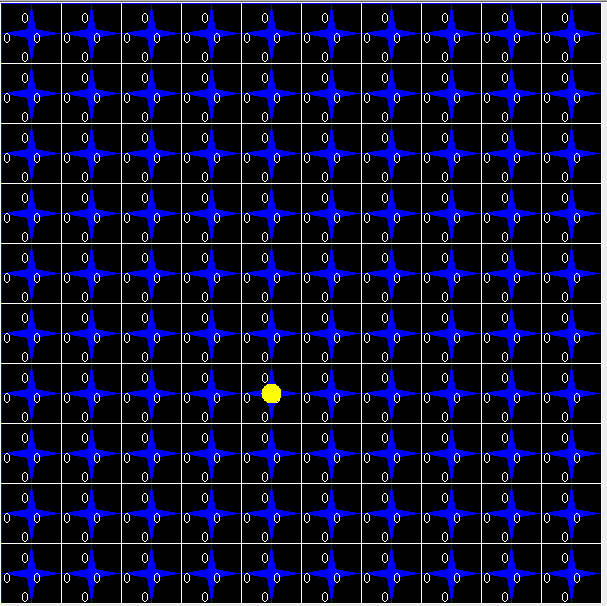
\includegraphics[width=0.7\textwidth]{./images/grid1.png}
\caption{Example of a simple MDP with three states and two actions}
\label{fig:mdp}
\end{figure}



There are 4 actions available: up, down, left and right. If it carries out one of these actions, it have a 0.7 chance of going one step in the desired direction and a 0.1 change in going one step in any of the other three directions. If it bumps into the outside wall (i.e., the square computed as above is outside the grid), there is a penalty on 1 (i.e., a reward of -1) and the agent doesn't actually move. When an agent acts in one of the states with positive reward, it is flung, at random, to one of the 4 corners of the grid world (no matter what action it does). Again this is the same as the value iteration applet.

The initial discount rate is 0.9. It is interesting to try the Q-learning at different discount rates (using the "Increment Discount" and "Decrement Discount" buttons, or just typing it in).




\chapter{Improving Stress Search Based Testing using Q-Learning and Hybrid Metaheuristic Approach}


\section{Hybrid Approach}

A large number of researchers have recognized the advantages and huge potential of building hybrid metaheuristics. The main motivation for creating hybrid metaheuristics is to exploit the complementary character of different optimization strategies. In fact, choosing an adequate combination of algorithms can be the key to achieving top performance in solving many hard optimization problems \cite{Puchinger2005} \cite{Blum2012}.

The proposed solution makes it possible to create a model that evolves during the test. The proposed solution model uses genetic algorithms, tabu search, and simulated annealing in two different approaches. The study initially investigated the use of these three algorithms. Subsequently, the study will focus in others Population-based and single point search metaheuristics. The first approach uses the three algorithms independently, and the second approach uses the three algorithms collaboratively (hybrid metaheuristic approach).

In the first approach , the algorithms do not share their best individuals among themselves. Each algorithm evolves in a separate way (Fig. \ref{fig:firstaproach}).


\begin{figure}[h]
\centering
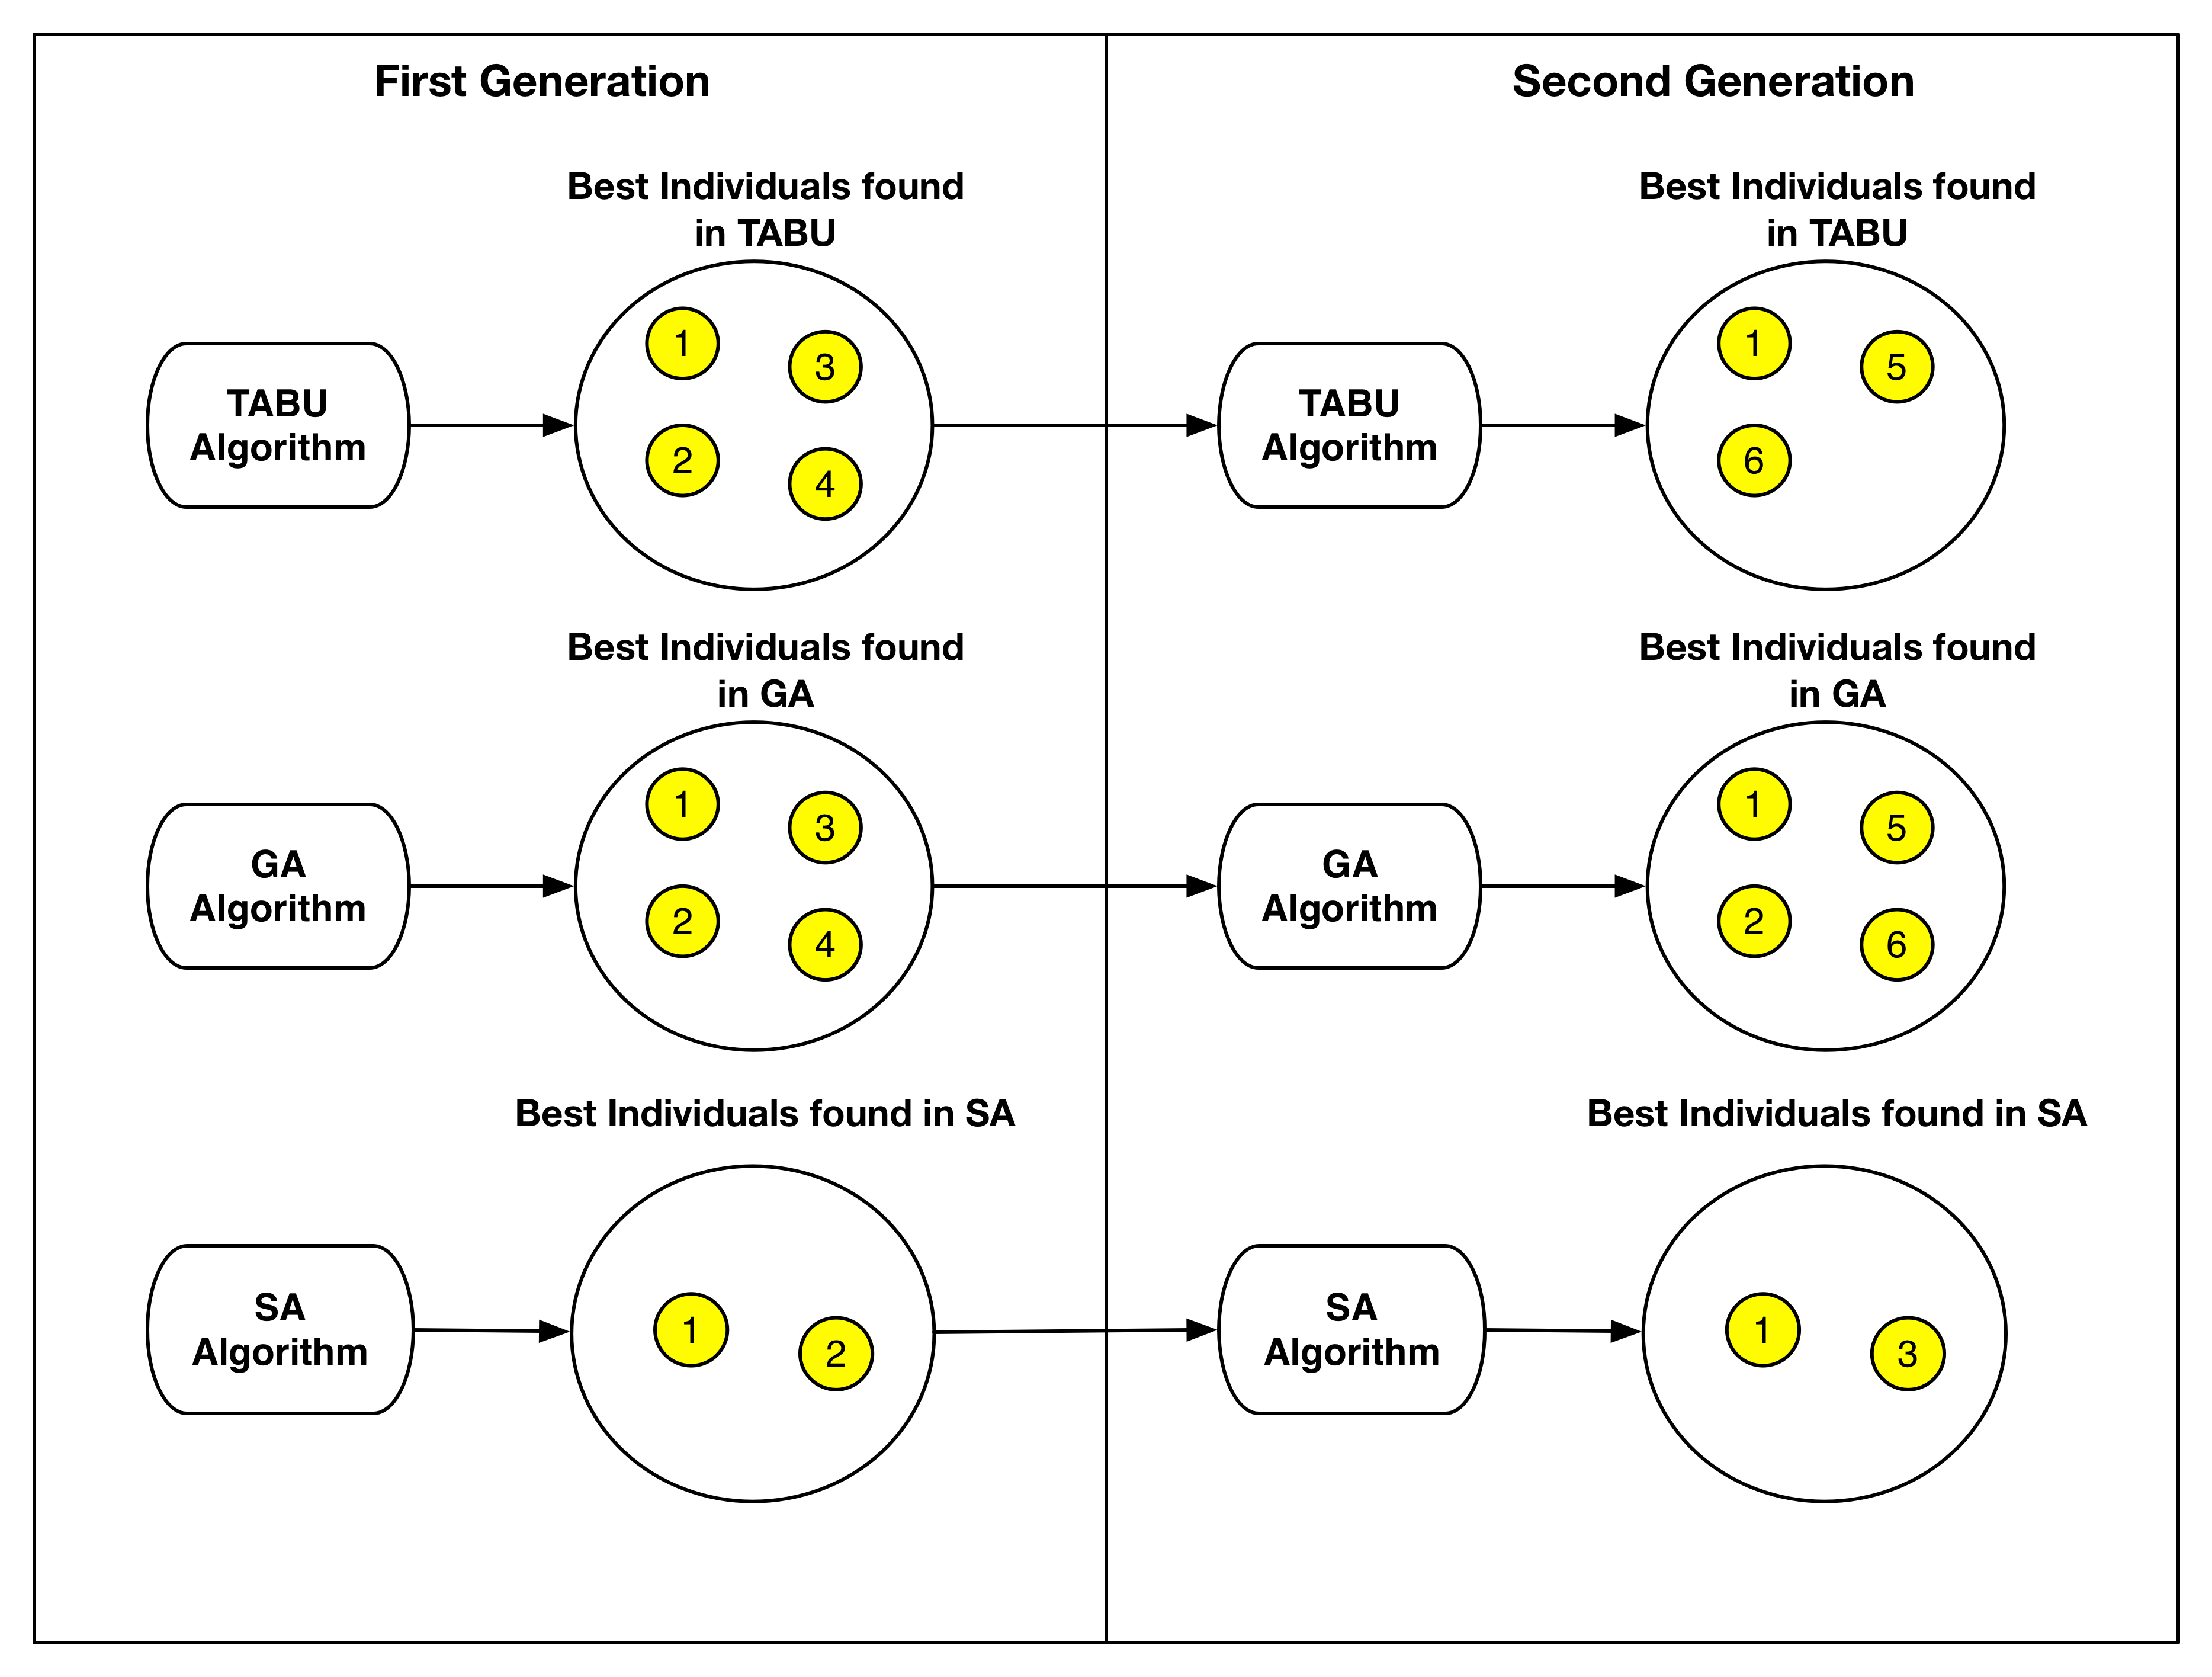
\includegraphics[width=0.7\textwidth]{./images/independ.png}
\caption{Use of the algorithms independently}
\label{fig:firstaproach}
\end{figure}



The second approach uses the algorithms in a collaborative mode (hybrid metaheuristic). In this approach, the three algorithms share their best individuals found (Fig. \ref{fig:secondapproach}). The next subsections present details about the used metaheuristic algorithms (Representation, initial population and fitness function).




\begin{figure}
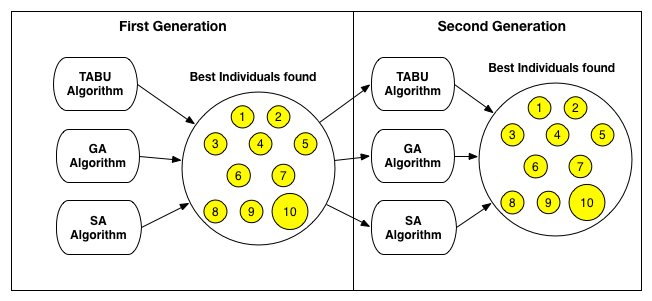
\includegraphics[width=1\textwidth]{./images/collaborative.png}
\caption{Use of the  algorithms collaboratively}
\label{fig:secondapproach}
\end{figure}

\subsection{Representation}

The solution representation is composed by a linear vector with 23 positions. The first position represents the name of an individual. The second position represents the algorithm (genetic algorithm, simulated annealing, or Tabu search) used by the individual. The third position represents the type of test (load, stress, or performance). The next positions represent 10 scenarios and their numbers of users. Each scenario is an atomic operation: the scenario must log into the application, run the task goal, and undo any changes performed, returning the application to its original state.

Fig. \ref{fig:genomarepresentation} presents the solution representation and an example using the crossover operation. In the example, genotype 1 has the Login scenario with 2 users, the Form scenario with 0 users, and the Search scenario with 3 users. Genotype 2 has the Delete scenario with 10 users, the Search scenario with 0 users, and the Include scenario with 5 users. After the crossover operation, we obtain a genotype with the Login scenario with 2 users, the Search scenario with 0 users, and the Include scenario with 5 users.

\begin{figure}[h]
\centering
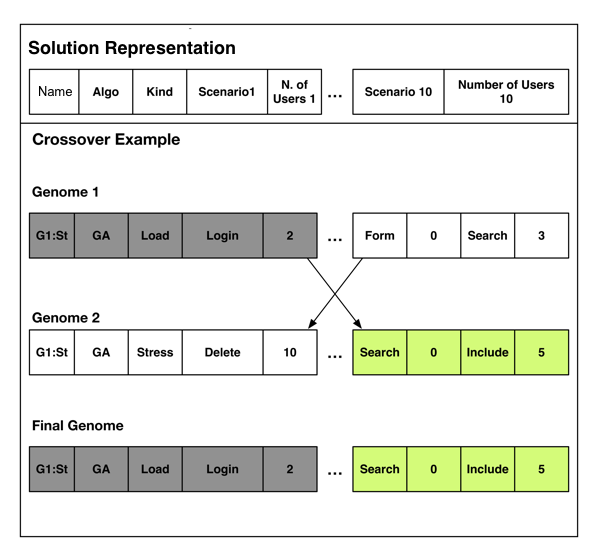
\includegraphics[width=1\textwidth]{./images/genomerepresentation1.png}
\caption{Solution representation and crossover example}
\label{fig:genomarepresentation}
\end{figure}

Fig. \ref{fig:neighbourtaby} shows the strategy used by the proposed solution to obtain the representation of the neighbors for the Tabu search and simulated annealing algorithms. The neighbors are obtained by the modification of a single position (scenario or number of users) in the vector.


\begin{figure}[h]
\centering
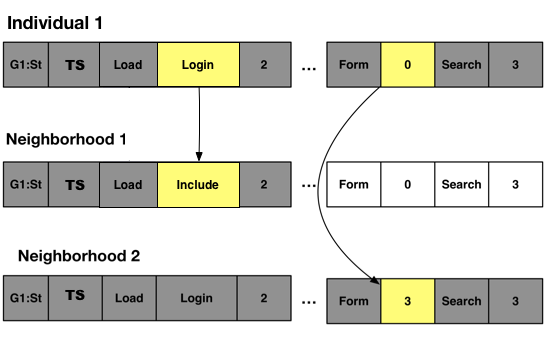
\includegraphics[width=1\textwidth]{./images/neighbor.png}
\caption{Tabu search and simulated annealing neighbor strategy}
\label{fig:neighbourtaby}
\end{figure}


\subsection{Initial population}

The strategy used by the plugin to instantiate the initial population is to generate 50\% of the individuals randomly, and 50\% of the initial population is distributed in three ranges of values:

\begin{itemize}
\item Thirty percent of the maximum allowed users in the test;
\item Sixty percent of the maximum allowed users in the test; and
\item Ninety percent of the maximum allowed users in the test.
\end{itemize}

The percentages relates to the distribution of the users in the initial test scenarios of the solution. For example, in a hypothetical test with 100 users, the solution will create initial test scenarios with 30, 60 and 90 users.

\subsection{Objective (fitness) function}

The proposed solution was designed to be used with independent testing teams in various situations where the teams have no direct access to the environment where the application under test was installed. Therefore, the IAdapter plugin uses a measurement approach to the definition of the fitness function. The fitness function applied to the IAdapter solution is governed by the following equation:

\begin{equation}
\begin{aligned}
fit=90percentileweigth* 90percentiletime\\
+80percentileweigth*80percentiletime\\+
70percentileweigth*70percentiletime+\\
maxResponseWeigth*maxResponseTime+\\
numberOfUsersWeigth*numberOfUsers-penalty
\end{aligned}
\end{equation}

The proposed solution's fitness function uses a series of manually adjustable user-defined weights (90percentileweight, 80percentileweight,  70percentileweight, maxResponseWeight, and numberOfUsersWeight). These weights make it possible to customize the search plugin's functionality. A penalty is applied when an application under test takes a longer time to respond than the level of service. The penalty is calculated by the follow equation:

\begin{equation}
\begin{aligned}
penalty=100 * \Delta \\
\Delta=(t_{Current Response Time} - t_{Maximum Response Time Expected})\\
\end{aligned}
\end{equation}


\section{IAdapter}

IAdapter is a JMeter plugin designed to perform search-based stress tests.  The plugin is available on www.iadapter.org.  The IAdapter plugin implements the solution proposed in Section 5. The next subsections present details about the Apache JMeter tool, the IAdapter Life Cycle and the IAdapter Components. The IAdapter plugin provides three main components: WorkLoadThreadGroup, WorkLoadSaver, and WorkLoadController.

The Fig. \ref{fig:iadapterarchitecture} show the IAdapter architecture. All metaheuristic class implements the interface IAlgorithm. Test scenarios  and test results are stored in a Mysql database. GeneticAlgorithm class uses a framework named JGAP to implement Genetic Algorithms.

\begin{figure}[h]
\center
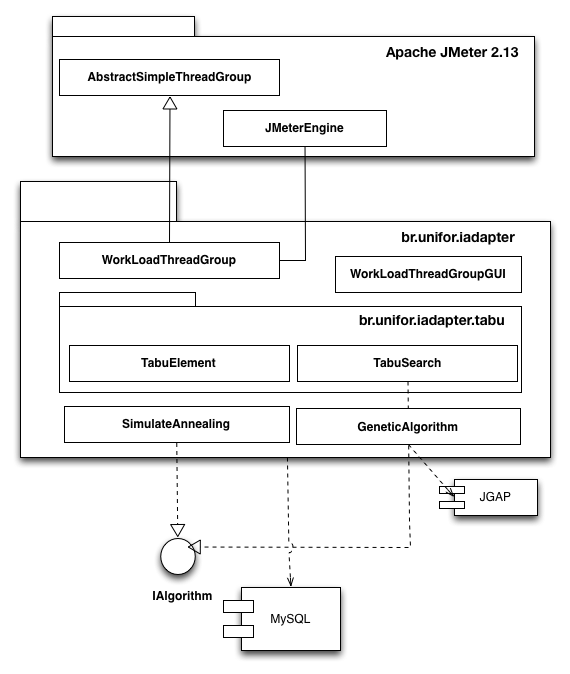
\includegraphics[width=0.8\textwidth]{./images/iadapter1.png}
\caption{IAdapter architecture}
\label{fig:iadapterarchitecture}
\end{figure}

The WorkLoadThreadGroup class is the Load Injection and Test Management modules, responsible to generate the initial population and uses the JMeter Engine to realize requests to server under test. 

\subsection{IAdapter Life Cycle}
 
Fig. \ref{fig:iadapterlifecycle} presents the IAdapter Life Cycle. The main difference between IAdapter and JMeter tool is that the IAdapter provide an automated test execution where the new test scenarios are choosen by the test tool.  In a test with JMeter, the tests scenarios are usually chosen by a test designer.

\begin{figure}[h]
\centering
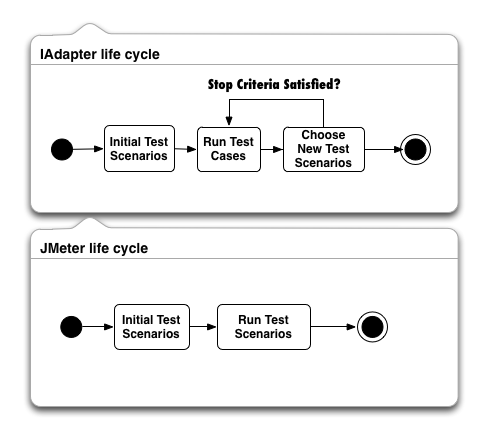
\includegraphics[width=0.8\textwidth]{./images/lifecycle2.png}
\caption{IAdapter life cycle}
\label{fig:iadapterlifecycle}
\end{figure}

\subsection{IAdapter Components}
 
WorkLoadThreadGroup is a component that creates an initial population and configures the algorithms used in IAdapter. Fig. \ref{fig:tela1iadapter} presents the main screen of the WorkLoadThreadGroup component. The component has a name \ding{202}, a set of configuration tabs \ding{203}, a list of individuals by generation \ding{204}, a button to generate an initial population \ding{205}, and a button to export the results \ding{206}.

\begin{figure}[h]
\centering
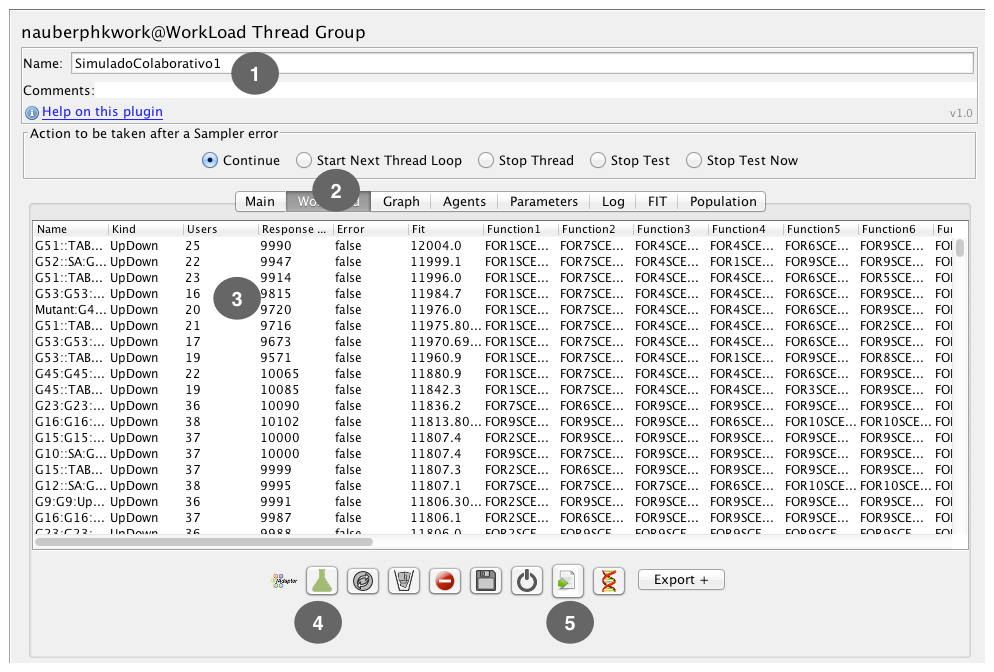
\includegraphics[width=0.8\textwidth]{./images/tela1iadapter.png}
\caption{WorkLoadThreadGroup component}
\label{fig:tela1iadapter}
\end{figure}

WorkLoadThreadGroup component uses the GeneticAlgorithm, TabuSearch and SimulateAnnealing classes.  The WorkLoadSaver component is responsible for saving all data in the database. The operation of the component only requires its inclusion in the test script.

WorkLoadController represents a scenario of the test. All actions necessary to test an application should be included in this component. All instances of the component need to login into the application under test and bring the application back to its original state.


\subsection{IAdapter Testbed Tool}

A Testbed makes possible follow a formalized methodology and reproduce tests for further analysis and comparison. It seems natural that one of the most important parts of a comparison among heuristics is the testbed on which the heuristics are tested. As a result, the testbed should be the first consideration when comparing two metaheuristics \cite{GendreauMichelandPotvin2010}. 

In this section, We devise a new testbed that has the ability to reproduce different types of web workloads.  The proposed solution extends the IAdapter  plugin to create a testbed tool to validade load, performance and stress search based tests approaches \cite{Gois2016}. The IAdapter is a JMeter plugin designed to perform search-based stress tests. 

This new testbed must accomplish three main goals. First, it must reproduce a workload by using an antipattern implementation. Second, it must be able to provide client and server metrics with the aim of being used for web performance evaluation studies. Finally, it is should be extensible, allowing create new test scenarios.

IAdapter Testbed is an open-source facility that provides software tools for search based test research. The testbed tool emulates test scenarios in a controled environment using mock objects and implementing performance antipatterns. 

The testbed tool proposed consists of four main elements. The first element is a emulator module that it is responsible to simulate the antipatterns in a specific context. The second it's a module named test module that it is responsible for use a previous selected metaheuristics and perform a search based test. The third module contains the test scenarios representation. The fourth module it is responsible for provide a service of explore the neighborhood of a given individual. 



\subsubsection{Testbed Architecture}


The Fig. \ref{fig:testbedarch} presents the main architecture of the Testbed solution proposed. The emulator module provides workloads to the Test module.The Test module uses a class loader to find all classes that extends AbstractAlgorithm in the classpath and run all tests for each metaheuristic found. The Test Scenario Representation and Persistent Module provides the scenario representation used by the metaheuristics and persist the testbed results data in a database. Neighborhood provider service is responsible to search neighbors of some individual provided as parameter to the service.

\begin{figure}[h]
\centering
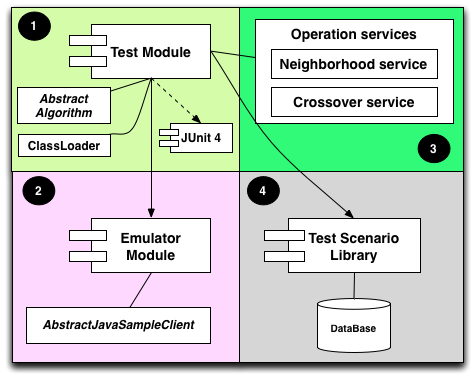
\includegraphics[width=1\textwidth]{./images/testbedarch.png}
\caption{testbed main architecture.}
\label{fig:testbedarch}
\end{figure} 

\begin{figure}[h]
\centering
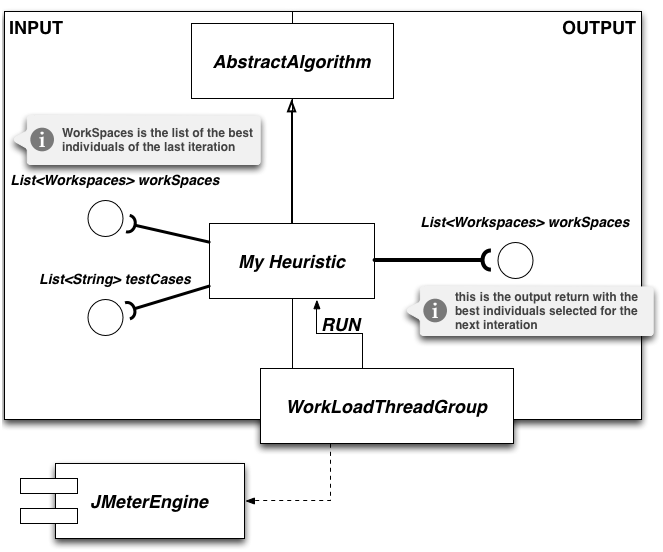
\includegraphics[width=0.8\textwidth]{./images/myheuristic.png}
\caption{Heuristic class diagram.}
\label{fig:heuristicclassdiagram}
\end{figure} 



\subsubsection{Test Module}

The Test Module is responsible for load all classes that extends AbstractAlgorithm in the classpath and perform the tests under the application. The Emulator Module provides successful scenarios and antipatterns implementations. The heuristics are executed in order to select the scenarios with failures or high response times. The Fig. \ref{fig:step1} presents the first feature of Test Module where a initial population it is created and IAdapter with JMeterEngine performs all tests and apply a fitness value to each workload.

\begin{figure}[h]
\begin{minipage}{.5\textwidth}
\centering
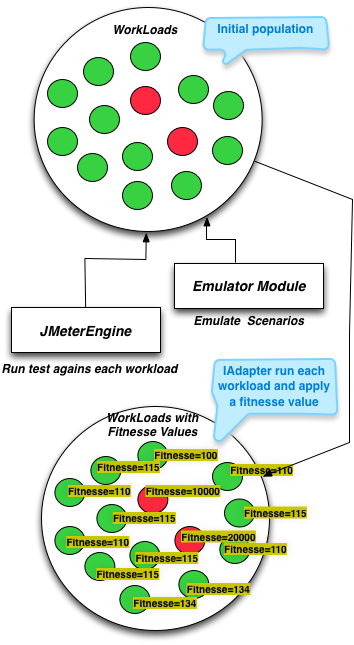
\includegraphics[width=1\textwidth]{./images/step1.png}
\caption{Test Module first feature.}
\label{fig:step1}
\end{minipage}
\begin{minipage}{.5\textwidth}
\centering
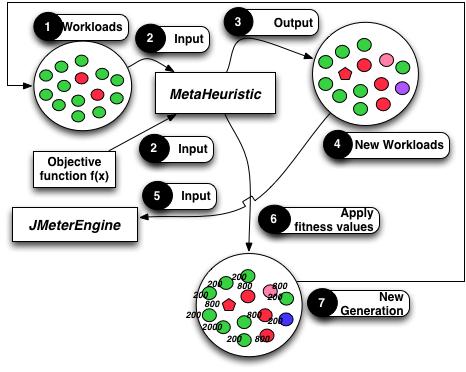
\includegraphics[width=1\textwidth]{./images/step2.png}
\caption{Test Module life cycle.}
\label{fig:step2}
\end{minipage}
\end{figure} 

The Fig. \ref{fig:step2} presents the Test Module life cycle. The life cycle iterate over two steps: The first step apply a metaheurist to select or generate a new set of workloads based on selection criteria. The second step run each workload with the JMeterEngine and obtain a fitness value based on some objective function. The red circles represent the workload that contain errors. The green circles represents the workloads with no errors and low acceptable response time. The testbed tool uses as default objective function the equation:


\begin{equation}
\begin{aligned}
fitness=90percentileweigth* 90percentiletime\\
+80percentileweigth*80percentiletime\\+
70percentileweigth*70percentiletime+\\
maxResponseWeigth*maxResponseTime+\\
numberOfUsersWeigth*numberOfUsers-penalty
\end{aligned}
\end{equation}

The use of presented fitness value by each metaheuristic it's optional. Each Metaheuristic could define your own objective function. The proposed  fitness function uses a series of manually adjustable user-defined weights (90percentileweight, 80percentileweight,  70percentileweight, maxResponseWeight, and numberOfUsersWeight). These weights make it possible to customize the search plugin's functionality. A penalty is applied when an application under test takes a longer time to respond than the level of service. After all these steps the cycle begins until the maximum number of generations it is reached. The Fig. \ref{fig:heuristicclassdiagram} shows the  class diagram for custom and provided heuristics. All heuristic classes extends the class AbstractAlgorithm. The heuristics receives  as input a  list of workspaces and a list of testcases. The workspace represents each individual in the search space.


Each metaheuristic class returns a list of workspaces (the individuals selected to the next generation). The Listing presents the method that performs the search of classes that extends Abstract Algorithm



\subsubsection{Emulator Module}

The Emulator Module is responsible for implement and provide successful scenarios and the most commons performance antipatterns. All classes must extends the AbstractJavaSamplerClient class or use JUnit 4. The AbstractJavaSamplerClient class allows create a JMeter Java Request.  Using JUnit 4, the emulators classes could be called by a JMeter JUnit request. The Fig. \ref{fig:emulator} presents the main features of the emulator module. The module implements 8 test scenarios in its first version.

\begin{figure}[h]
\centering
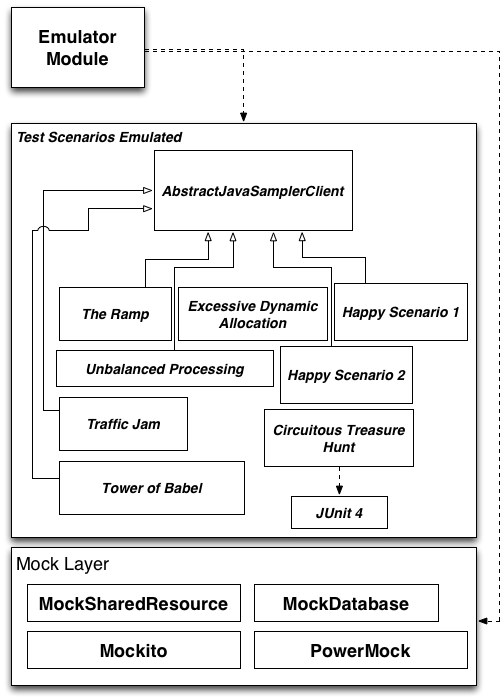
\includegraphics[width=0.7\textwidth]{./images/emulator.png}
\caption{Heuristic class diagram.}
\label{fig:emulator}
\end{figure}  

The Mock Layer provides emulated databases and components to the test scenarios. Each scenario provided by the Emulator Module could be called in JMeter using a Java Request. The algorithm \ref{unbalancedalgorithm} emulates the Unbalanced Processing antipattern. The test scenario C still waiting until A and B scenarios are used by a test.

\begin{algorithm}[H]
  \caption{Unbalanced Processing emulate algorithm}\label{unbalancedalgorithm}
  \begin{algorithmic}[1]
    
    \While{ List of processing scenarios contains A and B }
    \State Processing A and B scenarios
    \EndWhile
    \State Processing scenario C
      
  \end{algorithmic}
\end{algorithm}

The algorithm \ref{rampalgorithm} emulates  the Ramp antipattern. The algorithm increase the response time at each  time that it has been used.

\begin{algorithm}[H]
  \caption{The Ramp emulate algorithm}\label{rampalgorithm}
  \begin{algorithmic}[1]
    \If {count is null}
    \State $count \gets 0  $
    \EndIf
    \State sleep(100* count)
    \State $count \gets count +1  $     
  \end{algorithmic}
\end{algorithm}


The algorithm \ref{excessivedynamicallocation} implements the Excessive Dynamic Allocation antipattern. The algorithm creates a connection with a emulated database, uses the connection and finally the connection.

\begin{algorithm}[H]
  \caption{Excessive Dynamic Allocation emulate algorithm}\label{excessivedynamicallocation}
  \begin{algorithmic}[1]
    
    \For{\textbf{each} request}
        \For{int i=0 to 1000}
        \State Create a connection to a database
        \State Use the connection
        \State Destroy the created connection     
        \EndFor
    \EndFor
      
  \end{algorithmic}
\end{algorithm}

The algorithm \ref{happyscenario1} presents the Happy Scenario 1. The response time increases for every 10 users.

\begin{algorithm}[H]
  \caption{Happy Scenario 1 emulate algorithm}\label{happyscenario1}
  \begin{algorithmic}[1]
    \State sleep(2*users)   
  \end{algorithmic}
\end{algorithm}

\begin{algorithm}[H]
  \caption{Happy Scenario 2 emulate algorithm}\label{happyscenario2}
  \begin{algorithmic}[1]
    \State sleep(3*users)   
  \end{algorithmic}
\end{algorithm}

A further 4 algorithms were developed for the scenarios  Circuitous Treasure Hunt, Happy Scenario 2, Traffic Jam and Tower of Babel.


\chapter{Experiments}

In this section, We present the results of experiments which we carried out to verify the antipatterns  implementation, the fitness objective function and the metaheuristics used by the testbed tool. We conducted two experiments in order to verify the effectiveness of the testbed tool.

The experiments ran for 17 generations. The experiments used an initial population of 4 individuals by metaheuristic. The genetic algorithm used the top 10 individuals from each generation in the crossover operation. The Tabu list was configured with the size of 10 individuals and expired every 2 generations.  The mutation operation was applied to 10\% of the population on each generation. The experiments uses tabu search, genetic algorithms and the hybrid metaheuristic approach proposed by Gois et al. \cite{Gois2016}. The objective function applied is intended to maximize the number of users and minimize the response time of the scenarios being tested.  In this experiments, better fitness values meaning to find scenarios with more users and a low values of response time. A penalty is applied when the response time is greater than the  maximum response time expected. The experiments used the following fitness (goal) function. :

\begin{equation}
\begin{aligned}
fit=3000*numberOfUsers\\
-20* 90percentiletime\\
-20*80percentiletime\\
-20*70percentiletime\\
-20*maxResponseTime\\
-penalty
\end{aligned}
\end{equation}

The penalty is calculated by the follow equation:

\begin{equation}
\begin{aligned}
penalty=100 * \Delta \\
\Delta=(t_{Current Response Time} - t_{Maximum Response Time Expected})\\
\end{aligned}
\end{equation}

The experiments addresses:

\begin{itemize}
\item Validate the operation of the testbed tool.
\item Find the maximum number of users and the minimal response time.
\item Analyze and verify the best heuristics among those chosen to the experiments.
\end{itemize}


\subsection{Emulated Class Test Experiment}

The first experiment aimed to perform performance, load, and stress testing on a simulated component. The purpose of using a simulated component was to be able to perform a greater number of generations in a shorter time available and eliminate variables such as the use of databases and application servers. The first experiment used a test class  named SimulateConcurrentAccess. This class has a static variable named \textit{x} and a set of methods that use the variable in a synchronized context ( Listing \ref{classsimulated}). The experiment was executed using the JMeter Java Request Sampler Component with IAdapter.

\lstdefinestyle{outline}{
		language=Java,
         basicstyle=\scriptsize\ttfamily,
         numberstyle=\tiny,
         numbersep=5pt,
         tabsize=2,
         extendedchars=true,
         breaklines=true,
         keywordstyle=\color{black}\bf,
         frame=b,  % <<<<<<<<<<<<<<<<<<<<<<<<<<
         stringstyle=\color{green!40!black}\ttfamily,
         showspaces=false,
         showtabs=false,
         numbers=left,
         xleftmargin=17pt,
         framexleftmargin=17pt,
         framextopmargin=1pt, % <<<<<<<<<<<<<<<<<<<<<<
         showstringspaces=false,
         %backgroundcolor=\color[RGB]{200,200,200},
         belowcaptionskip=0pt
}

\begin{lstlisting}[style=outline,caption={SimulateConcurrentAccess class},float,label=classsimulated]
public class SimulateConcurrentAccess {
  @Test
  public void firstScenario() {		
    synchronized (StaticClass.class) {
			for (int i = 0; i <= 1000; i++) {
				StaticClass.x += i;
			}
			StaticClass.x = 0;
		}
	}
	
	  @Test
  public void secondScenario() {		
    synchronized (StaticClass.class) {
			for (int i = 0; i <= 2000; i++) {
				StaticClass.x += i;
			}
			StaticClass.x = 0;
		}
	}
\end{lstlisting}


Fig.\ref{fig:exp1bestresults} presents the best results in 27 generations applied in the first experiment. The figure shows the results obtained with the algorithms with and without collaboration. The $x$ axis  represents the generation number, and the $y$ axis represents the best fitness value obtained until the current generation.
A higher value in the figure means that the scenario has a greater response time by the application under test. The results of the experiment showed that the use of cooperation between the three algorithms resulted in finding the individuals with better fitness values.

\begin{figure}[h]
\centering
\caption{Best results obtained in 27 generations}
\includegraphics[width=1\textwidth]{./images/generationcomparative.png}
\label{fig:exp1bestresults}
\end{figure}

Table \ref{tab:averagefirst} presents the results obtained by the hybrid metaheuristic (HM) approach, genetic algorithm (GA), simulated annealing (SA), and Tabu search (TS) from 27 generations in the first experiment. The values are the maximum fitness value obtained by each algorithm. 

\begin{table}[h]
\centering
\caption{Maximum value of the fitness function by algorithm}
\label{tab:averagefirst}
\begin{tabular}{|l|l|l|l|l|}
\hline
GEN & HM & TS  & GA    & SA    \\ \hline
1          & 11238 & 11238         & 11238 & 11238 \\ \hline
2          & 11804 & 11596         & 11801 & 10677 \\ \hline
3          & 11787 & 8932          & 8411  & 10869 \\ \hline
4          & 11723 & 9753          & 9611  & 10760 \\ \hline
5          & 8164  & 9780          & 10738 & 4794  \\ \hline
6          & 11802 & 9781          & 11086 & 6120  \\ \hline
7          & 9985  & 5782          & 11272 & 11798 \\ \hline
8          & 11803 & 11749         & 10084 & 11309 \\ \hline
9          & 11806 & 7284          & 11633 & 10766 \\ \hline
10         & 11807 & 9386          & 11717 & 4557  \\ \hline
11         & 11802 & 9653          & 11802 & 11151 \\ \hline
12         & 11807 & 10594         & 11793 & 9434  \\ \hline
13         & 11802 & 10848         & 10382 & 11805 \\ \hline
14         & 11801 & 11551         & 7219  & 10237 \\ \hline
15         & 11807 & 1701          & 7189  & 9338  \\ \hline
16         & 11813 & 6203          & 11758 & 5321  \\ \hline
17         & 11805 & 10720         & 10805 & 11748 \\ \hline
18         & 9600  & 6371          & 11698 & 7818  \\ \hline
19         & 11733 & 8160          & 11648 & 11509 \\ \hline
20         & 9589  & 9428          & 11805 & 4813  \\ \hline
21         & 11800 & 9463          & 11798 & 10801 \\ \hline
22         & 11805 & 11799         & 11804 & 6029  \\ \hline
23         & 11836 & 11655         & 11800 & 3579  \\ \hline
24         & 11805 & 11512         & 11803 & 5761  \\ \hline
25         & 11804 & 11573         & 11802 & 9680  \\ \hline
26         & 11800 & 11575         & 11403 & 9388  \\ \hline
27         & 11805 & 10691         & 11745 & 9465  \\ \hline
\end{tabular}
\end{table}

The signed-rank Wilcoxon non-parametrical procedure was used for comparing the results with Z-value and W-value. The significant level adopted was 0.05. The Z-value obtained was -2.2736 and the p-value was 0.0232. The W-value obtained was 78. The critical value of W for N = 25 at p$$ 0.05 was 89.The result was significant at p$$ 0.05. The procedure showed that there was a significant improvement in the results with the collaborative approach.

\section{The Ramp and Circuitous Treasure Hunt experiment}

The experiment was carried out for 8 continuous hours.  All tests in the experiment were conducted without the need of a tester, automating the process of executing and designing performance test scenarios.In this experiment, Scenarios were generated with the Ramp and Circuitous Treasure antipattern as well as scenarios with Happy Scenario 1, Happy Scenario 2 and mixed scenarios. The Fig. \ref{fig:fitnessbygeneration1} and \ref{fig:fitnessbygeneration1-2} presents the fitness value obtained by each metaheuristic. The SA algorithm obtained the worst fitness values. Hybrid metaheuristic obtained the better fitness values. 


\begin{figure}[H]

\centering
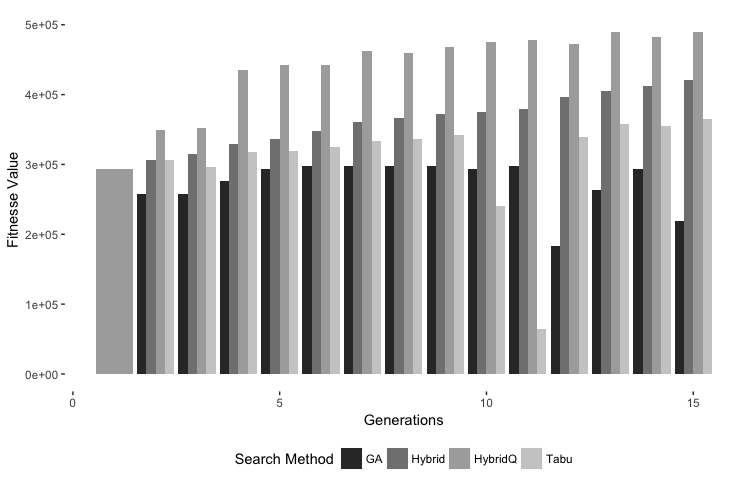
\includegraphics[width=0.7\textwidth]{./images/experiment1-1.png}
\caption{fitness value obtained by Search Method }
\label{fig:fitnessbygeneration1}
\end{figure}



\begin{figure}[H]
\centering
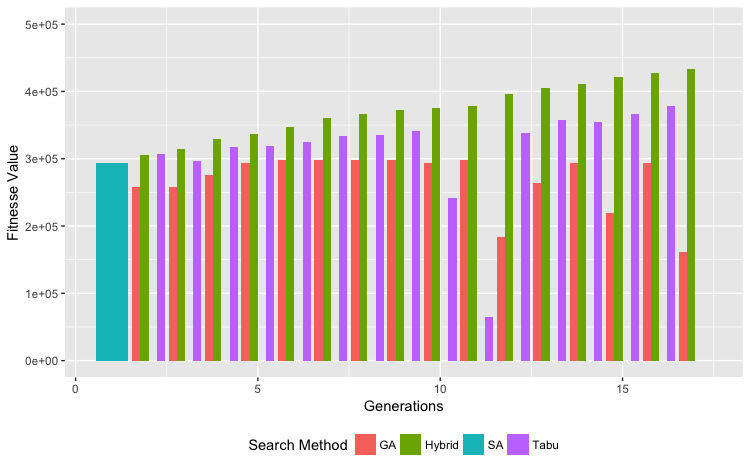
\includegraphics[width=0.7\textwidth]{./images/experiment1-2.png}
\caption{fitness value obtained by Search Method without SA metaheuristic.}
\label{fig:fitnessbygeneration1-2}

\end{figure}

Despite having obtained the best fitness value in each generation, the Hybrid algorithm performs twice as many requests as the second one, the tabu search (Fig. \ref{fig:numberofrequestsbysearchmethod}). The Fig. \ref{fig:boxplot1} shows the average, minimal e maximum value by search method.


\begin{figure}[H]

\centering
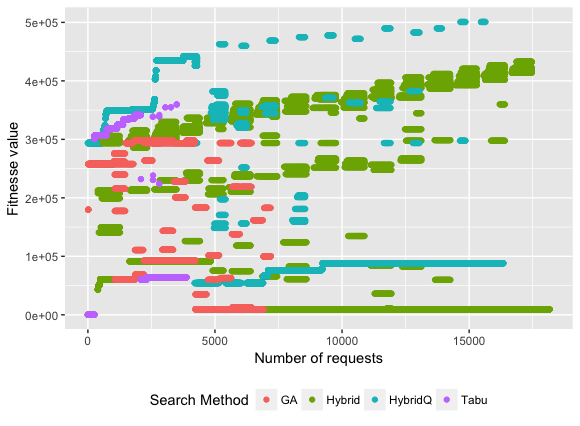
\includegraphics[width=0.8\textwidth]{./images/experiment1-3.png}
\caption{Number of requests by Search Method}
\label{fig:numberofrequestsbysearchmethod}
\end{figure}
\begin{figure}[H]
\centering
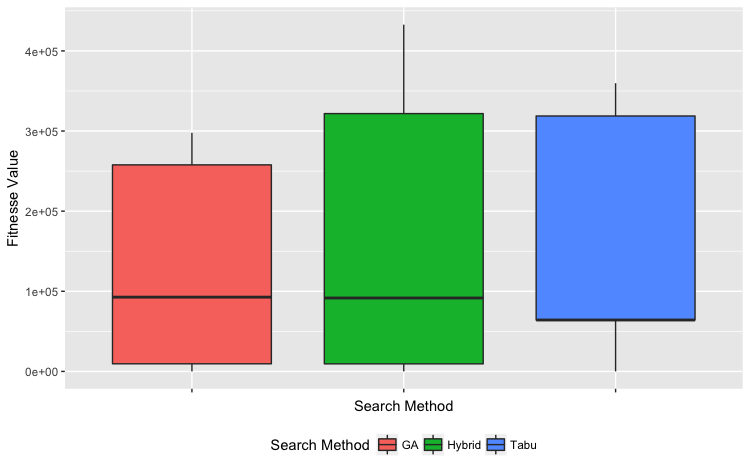
\includegraphics[width=0.8\textwidth]{./images/experiment1-4.png}
\caption{Average, median, maximum and minimal fitness value by Search Method}
\label{fig:boxplot1}

\end{figure}

The Fig. \ref{fig:summaryboxplot1} presents the maximum, average, median and minimum fitness value by generation. The maximun fitness value increases at each generation. The Fig. \ref{fig:density1} presents the density graph of number of users by fitness value. The range between 100 and 150 users has the highest number of individuals found with higher fitness value.

\begin{figure}[H]

\centering
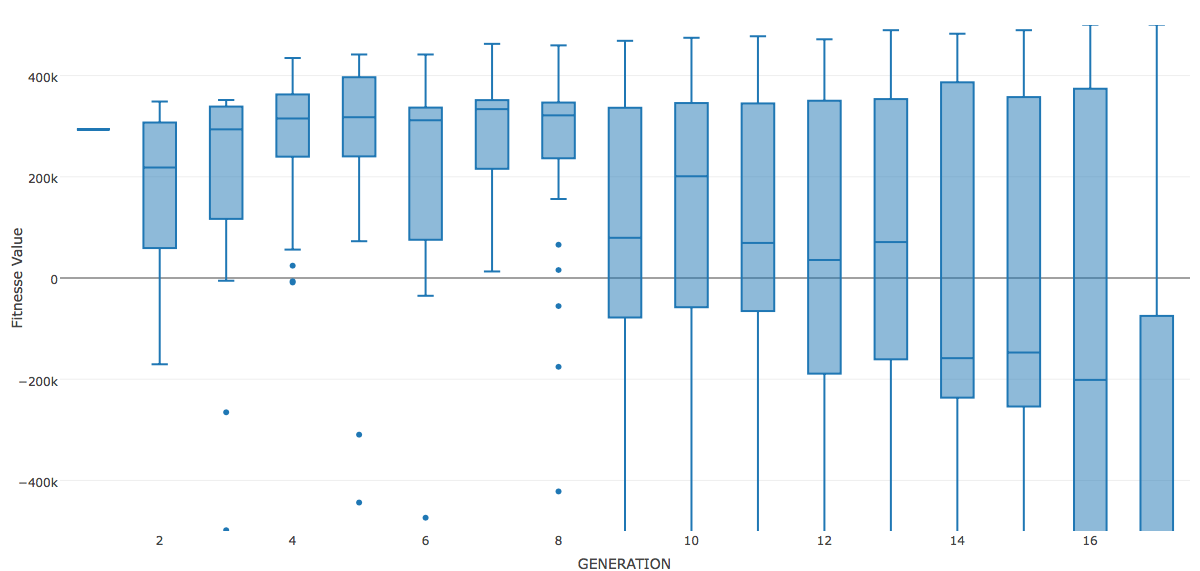
\includegraphics[width=1\textwidth]{./images/experiment1-5.png}
\caption{fitness value by generation}
\label{fig:summaryboxplot1}
\end{figure}
\begin{figure}[H]
\centering
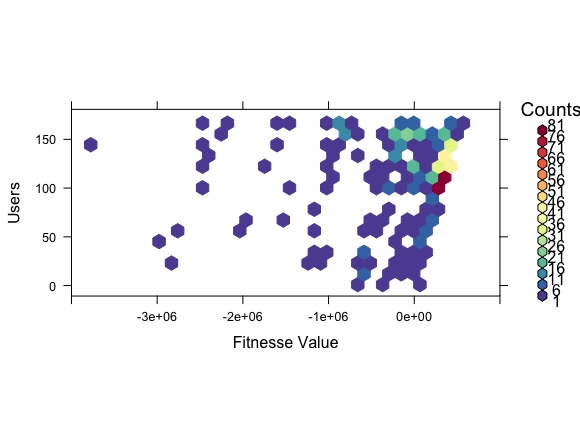
\includegraphics[width=1\textwidth]{./images/experiment1-6.png}
\caption{Density graph of number of users by fitness value}
\label{fig:density1}

\end{figure}

Table \ref{tab:bestindividuals} shows 4 individuals with 143 to 146 users. These are the scenarios with the maximum number of users found with the best response time. The first individual has 64 users on Happy Scenario 2, 81 users on Happy Scenario 1 and a response time of 12 seconds. None of the best individuals has one of the antipatterns used in the experiment.



% Please add the following required packages to your document preamble:
% \usepackage[table,xcdraw]{xcolor}
% If you use beamer only pass "xcolor=table" option, i.e. \documentclass[xcolor=table]{beamer}
\begin{table}[h]
\centering
\caption{Best individuals found in the first experiment}
\label{tab:bestindividuals}
\begin{tabular}{lllllll}
\rowcolor[HTML]{C0C0C0} 
\textbf{Search Method} & \textbf{Generation} & \textbf{Users} & \textbf{fitness Value} & \textbf{Happy 2} & \textbf{Happy 1} & \textbf{Response Time} \\
Hybrid & 17 & 145 & 432760 & 64 & 81 & 12 \\
Hybrid & 17 & 145 & 432740 & 46 & 99 & 13 \\
Hybrid & 17 & 146 & 431760 & 54 & 92 & 12 \\
Hybrid & 16 & 143 & 426740 & 30 & 113 & 13
\end{tabular}
\end{table}

Fig. \ref{fig:responsetimegenerationalltests1} presents the response time by number of users of individuals with Happy Scenario 1 and Happy Scenario 2. The Figure illustrates that the individuals with best fitness value has more users and minor response time. The Fig. \ref{fig:fitnessgenerationalltests1-1} presents the response time by number of users of individuals with the Ramp and Circuitous Treasure antipatterns scenarios. The Figure illustrates the smallest number of individuals with the antipatterns when compared to individuals who use the happy scenarios.


\begin{figure}[H]
\centering
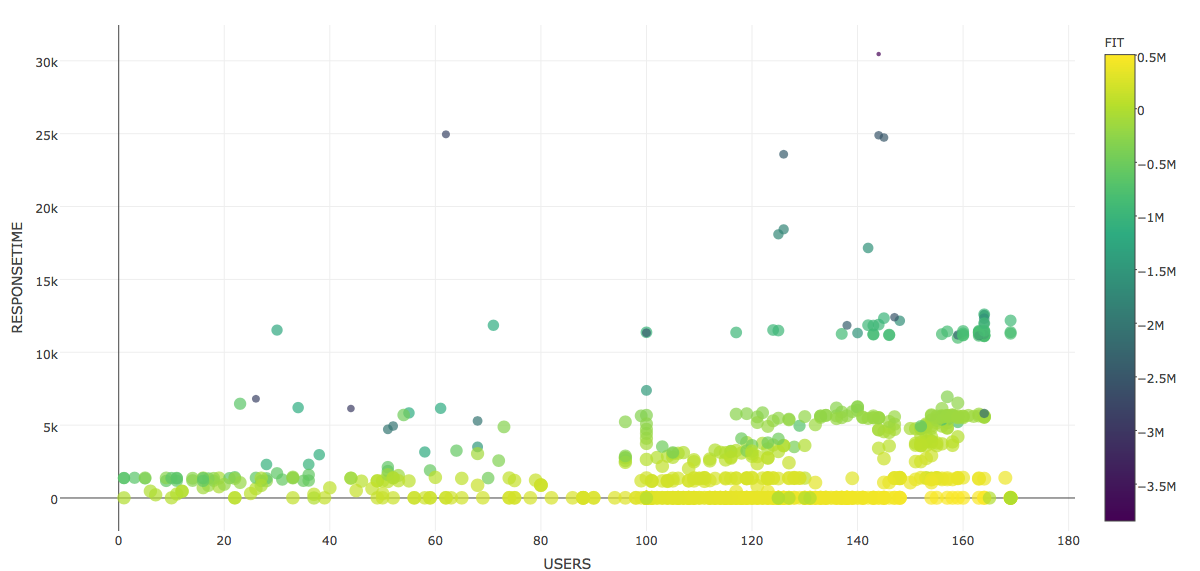
\includegraphics[width=1\textwidth]{./images/experiment1-7.png}
\caption{Response time by number of users of individuals with Happy Scenario 1 and Happy Scenario 2}
\label{fig:responsetimegenerationalltests1}
\end{figure}


\begin{figure}[H]
\centering
\includegraphics[width=1\textwidth]{./images/experiment1-8.png}
\caption{Response time by number of users of individuals with the Ramp and Circuitous Treasure antipatterns}
\label{fig:fitnessgenerationalltests1-1}

\end{figure}

In the first experiment, We conclude that the metaheuristics converged to scenarios with an happy path, excluding the scenarios with antipatterns. The hybrid metaheuristic returned individuals with higher fitness scores. However, the Hybrid metaheuristic made twice as many requests than Tabu Search to overcome it. The SA algorithm obtained the worst fitness values. The algorithm initially used a scenario with the Ramp and Circuitous Treasure antipatterns  and found neighbors that still using the antipatterns over the 17 generations of the experiment.




\FloatBarrier
\section{The Tower Babel  and Unbalanced Processing experiment}

The experiment was carried out for 6 continuous hours. All tests in the experiment were conducted without the need of a tester. In this experiment, Scenarios were generated with Tower Babel and Unbalanced Processing antipattern as well as scenarios with Happy Scenario 1, Happy Scenario 2 and mixed scenarios. The Fig. \ref{fig:fitnessbygeneration2}  presents the fitness value obtained by each metaheuristic. The SA algorithm obtained the worst fitness values. Hybrid metaheuristic obtained the better fitness values.


\begin{figure}[h]
\centering
\includegraphics[width=.9\textwidth]{./images/experiment2-7.png}
\caption{itnesse value obtained by Search Method}
\label{fig:fitnessbygeneration2}
\end{figure}

As in the first experiment, the Hybrid algorithm performs twice as many requests as the second one, the tabu search (Fig. \ref{fig:numberofrequestsbysearchmethod2}). The Fig. \ref{fig:boxplot2} shows the average, minimal e maximum value by search method. The Fig. \ref{fig:summaryboxplot2} presents the maximum, average, median and minimum fitness value by generation. The maximun fitness value increases at each generation. The Fig. \ref{fig:density2} presents the density graph of number of users by fitness value. The range between 100 and 150 users has the highest number of individuals found with higher fitness value.


\begin{figure}[h]
\begin{minipage}{.5\textwidth}
\centering
\includegraphics[width=1\textwidth]{./images/experiment2-1.png}
\caption{Number of requests by Search Method}
\label{fig:numberofrequestsbysearchmethod2}
\end{minipage}
\begin{minipage}{.5\textwidth}
\centering
\includegraphics[width=1\textwidth]{./images/experiment2-2.png}
\caption{Finesse value by generation in all tests}
\label{fig:boxplot2}
\end{minipage}

\end{figure}



\begin{figure}[h]
\begin{minipage}{.5\textwidth}
\centering
\includegraphics[width=1\textwidth]{./images/experiment2-3.png}
\caption{Response time by generation in all tests scenarios}
\label{fig:summaryboxplot2}
\end{minipage}
\begin{minipage}{.5\textwidth}
\centering
\includegraphics[width=1\textwidth]{./images/experiment2-4.png}
\caption{Finesse value by generation in all tests}
\label{fig:density2}
\end{minipage}

\end{figure}

Table \ref{tab:bestindividuals2} shows 4 individuals with 145 to 148 users.  The first individual has 72 users on Happy Scenario 2, 30 users on Happy Scenario 1, 46 user with the antipattern Tower Babel and a response time of 11 seconds. Despite the fact of doing 300 conversions of the JSON standard for XML. The antipattern implementation does not return a much higher response time than happy paths. While happy paths returns from 10 to 15 seconds from a single user, Tower Babel antipattern has a response time of 10 to 29 seconds. None of the best individuals found implements the Unbalanced Processing antipattern.

Fig. \ref{fig:responsetimegenerationalltests2} presents the response time by number of users of individuals with Happy Scenario 1 and Happy Scenario 2. The Figure illustrates that the individuals with best fitness value has more users and minor response time. The Fig. \ref{fig:fitnessgenerationalltests2-1} presents the response time by number of users of individuals with with Unbalanced Processing antipatterns scenarios. The Figure illustrates the smallest number of individuals with the  Unbalanced Processing antipattern when compared to individuals who use the happy scenarios and the Tower Babel antipattern.



\begin{figure}[h]
\centering
\includegraphics[width=1\textwidth]{./images/experiment2-5.png}
\caption{Response time by number of users of individuals with Happy Scenario 1, Happy Scenario 2 and Tower Babel antipattern}
\label{fig:responsetimegenerationalltests2}
\end{figure}


\begin{figure}[h]
\centering
\includegraphics[width=1\textwidth]{./images/experiment2-6.png}
\caption{Response time by number of users of individuals with Unbalanced Processing antipattern}
\label{fig:fitnessgenerationalltests2-1}
\end{figure}


We conclude that the metaheuristics converged to scenarios with an happy path and Tower Babel antipattern, excluding the scenarios with Unbalanced Processing antipattern. The hybrid metaheuristic returned individuals with higher fitness scores. However, the Hybrid metaheuristic made twice as many requests than Tabu Search to overcome it. The SA algorithm obtained the worst fitness values. The algorithm initially used a scenario with an antipattern and found neighbors that still using an antipattern over the 17 generations of the experiment. The individual with best fitness value has 72 users on Happy Scenario 2, 30 users on Happy Scenario 1, 46 user with the antipattern Tower Babel and a response time of 11 seconds.

% Please add the following required packages to your document preamble:
% \usepackage[table,xcdraw]{xcolor}
% If you use beamer only pass "xcolor=table" option, i.e. \documentclass[xcolor=table]{beamer}
\begin{table}[h]
\centering
\caption{Best individuals found in the second experiment}
\label{tab:bestindividuals2}
\begin{tabular}{llllllll}
\rowcolor[HTML]{FFCCC9} 
\textbf{Search Method} & \textbf{Generation} & \textbf{Users} & \textbf{fitness Value} & \textbf{Happy 2} & \textbf{Tower} & \textbf{Happy 1} & \textbf{Time} \\ 
\multicolumn{1}{l}{Hybrid} & \multicolumn{1}{l}{17} & \multicolumn{1}{l}{148} & \multicolumn{1}{l}{437780} & \multicolumn{1}{l}{72} & \multicolumn{1}{l}{46} & \multicolumn{1}{l}{30} & \multicolumn{1}{l}{11} \\ 
\multicolumn{1}{l}{Hybrid} & \multicolumn{1}{l}{17} & \multicolumn{1}{l}{145} & \multicolumn{1}{l}{432740} & \multicolumn{1}{l}{71} & \multicolumn{1}{l}{15} & \multicolumn{1}{l}{59} & \multicolumn{1}{l}{13} \\ 
\multicolumn{1}{l}{Hybrid} & \multicolumn{1}{l}{16} & \multicolumn{1}{l}{146} & \multicolumn{1}{l}{431800} & \multicolumn{1}{l}{72} & \multicolumn{1}{l}{31} & \multicolumn{1}{l}{43} & \multicolumn{1}{l}{10} \\ 
\multicolumn{1}{l}{Hybrid} & \multicolumn{1}{l}{17} & \multicolumn{1}{l}{145} & \multicolumn{1}{l}{428780} & \multicolumn{1}{l}{71} & \multicolumn{1}{l}{32} & \multicolumn{1}{l}{42} & \multicolumn{1}{l}{11} \\ 
\end{tabular}
\end{table}

\subsection{Moodle Application Experiment}

This experiment used a Moodle application installed in a machine with 500 GB of hard disk space and 8 GB of memory. The study used six application scenarios:

\begin{itemize}
\item PostDeleteMessage: This scenario posts and deletes messages in the Moodle application.
\item MyHome: This scenario accesses the homepage of the user's application.
\item Login: This scenario is responsible for user authentication by the application.
\item Notifications: This scenario involves entering the notification page of each user.
\item Start Page: This scenario shows the initial start page of the application.
\item Badge: This scenario involves entering the badge page.
\end{itemize}

The maximum tolerated response time in the test was 30 seconds.  Any  individuals who obtained a time longer than the stipulated maximum time suffered penalties.  The whole process of stress and performance tests, which took 3 days and about 1800 executions, was carried out without the need for monitoring by a test designer. The tool automatically selected the next scenarios to be run up to the limit of six generations previously established. 

Table \ref{tab:secondexperiment} presents the maximum fitness value obtained by the hybrid metaheuristic (HM) approach, genetic algorithm (GA), simulated annealing (SA), and Tabu search (TS) in each generation. 


\begin{table}[h]
\centering
\caption{Results obtained from the second experiment}
\label{tab:secondexperiment}
\begin{tabular}{|l|l|l|l|l|}
\hline
GEN & HM    & TS    & GA    & SA    \\
\hline
1          & 32242 & 32242 & 32242 & 32242 \\
\hline
2          & 34599 & 32443 & 26290 & 35635 \\
\hline
3          & 35800 & 34896 & 34584 & 34248 \\
\hline
4          & 35782 & 34912 & 32689 & 25753 \\
\hline
5          & 35611 & 31833 & 34631 & 8366  \\
\hline
6          & 35362 & 35041 & 33397 & 9706 \\
\hline
\end{tabular}
\end{table}


The small number of samples of the experiment is insufficient to give a statistical significance to the results of the Wilcoxon procedure. However, it is noted that, in four of six generations, the collaborative approach presented the best values. The experiment succeeded in finding 29 individuals whose maximum time expected by the application was obtained.  Table \ref{tab:secondexperiment1} shows an example of the six individuals with the highest fitness values in the second experiment. The table shows the fitness value (Fit);  the name of the scenario (Scenario); the number of users (Users); and the percentiles of 90\%, 80\%, and 70\% (90per, 80per and 70per) in seconds.  

% Please add the following required packages to your document preamble:
% \usepackage{multirow}
\begin{table}[h]
\centering
\caption{Example of individuals obtained in the second experiment}
\label{tab:secondexperiment1}
\begin{tabular}{|p{0.2cm}|l|l|l|p{1.00cm}|p{1.00cm}|p{1.00cm}|}
\hline
Id&Fit&Scenario&Users&90per&80per&70per\\ \hline
\multirow{2}{*}{1} & \multirow{2}{*}{35800} & MyHome        & 31              & \multirow{2}{*}{30} & \multirow{2}{*}{29} & \multirow{2}{*}{10} \\ \cline{3-4}
                   &                        & Badges        & 4               &                     &                     &                     \\ \hline
\multirow{3}{*}{2} & \multirow{3}{*}{35795} & MyHome        & 30              & \multirow{3}{*}{30} & \multirow{3}{*}{29} & \multirow{3}{*}{10} \\ \cline{3-4}
                   &                        & Notifications & 2               &                     &                     &                     \\ \cline{3-4}
                   &                        & Badges        & 2               &                     &                     &                     \\ \hline
\multirow{2}{*}{3} & \multirow{2}{*}{35782} & MyHome        & 32              & \multirow{2}{*}{30} & \multirow{2}{*}{29} & \multirow{2}{*}{10} \\ \cline{3-4}
                   &                        & Badges        & 3               &                     &                     &                     \\ \hline
\multirow{3}{*}{4} & \multirow{3}{*}{35773} & MyHome        & 22              & \multirow{3}{*}{30} & \multirow{3}{*}{29} & \multirow{3}{*}{10} \\ \cline{3-4}
                   &                        & Notifications & 6               &                     &                     &                     \\ \cline{3-4}
                   &                        & Badges        & 9               &                     &                     &                     \\ \hline
\multirow{2}{*}{5} & \multirow{2}{*}{35771} & MyHome        & 28              & \multirow{2}{*}{30} & \multirow{2}{*}{29} & \multirow{2}{*}{9}  \\ \cline{3-4}
                   &                        & Badges        & 6               &                     &                     &                     \\ \hline
\multirow{2}{*}{6} & \multirow{2}{*}{35683} & MyHome        & 27              & \multirow{2}{*}{30} & \multirow{2}{*}{29} & \multirow{2}{*}{8}  \\ \cline{3-4}
                   &                        & Badges        & 10              &                     &                     &                     \\ \hline
\end{tabular}
\end{table}


Table \ref{fig:gened} presents the percentage of genes in all test scenarios by generation with and without collaboration. Most of the genes converged to the MyHome feature, which had the highest application response time.


% Please add the following required packages to your document preamble:
% \usepackage[table,xcdraw]{xcolor}
% If you use beamer only pass "xcolor=table" option, i.e. \documentclass[xcolor=table]{beamer}
\begin{table}[h]
\centering
\caption{Percentage of genes in each scenario by generation }
\label{fig:gened}
\begin{tabular}{c|c|c|c|c|c|c|c|}
\hline
\rowcolor[HTML]{D3D3D3} 
\multicolumn{1}{|c|}{\cellcolor[HTML]{FFFFFF}\textbf{Gen/}}   & \multicolumn{7}{c|}{\cellcolor[HTML]{D3D3D3}\textbf{Non collaboration approach}}                                                                                                                                                       \\ \cline{2-8} 
\multicolumn{1}{|c|}{\textbf{Scenarios}}                      & \cellcolor[HTML]{F8FF00}Initial & \cellcolor[HTML]{F8FF00}1 & \cellcolor[HTML]{F8FF00}2 & \cellcolor[HTML]{F8FF00}3 & \cellcolor[HTML]{F8FF00}4 & \cellcolor[HTML]{F8FF00}5 & \cellcolor[HTML]{F8FF00}6                                \\ \hline
\multicolumn{1}{|c|}{\cellcolor[HTML]{D3D3D3}Badges}          & 20                              & 18                        & 16                        & 24                        & 15                        & 16                        & 17                                                       \\ \hline
\rowcolor[HTML]{F8FF00} 
\multicolumn{1}{|c|}{\cellcolor[HTML]{F8FF00}\textbf{MyHome}} & \textbf{15}                     & \textbf{59}               & \textbf{55}               & \textbf{48}               & \textbf{53}               & \textbf{50}               & \multicolumn{1}{l|}{\cellcolor[HTML]{F8FF00}\textbf{52}} \\ \hline
\multicolumn{1}{|c|}{\cellcolor[HTML]{D3D3D3}StartPage}       & 15                              & 10                        & 12                        & 11                        & 20                        & 18                        & \multicolumn{1}{l|}{19}                                  \\ \hline
\multicolumn{1}{|c|}{\cellcolor[HTML]{D3D3D3}Notifications}   & 25                              & 5                         & 11                        & 10                        & 9                         & 10                        & \multicolumn{1}{l|}{9}                                   \\ \hline
\multicolumn{1}{|c|}{\cellcolor[HTML]{D3D3D3}Post}            & 8                               & 3                         & 1                         & 3                         & 1                         & 2                         & \multicolumn{1}{l|}{1}                                   \\ \hline
\multicolumn{1}{|c|}{\cellcolor[HTML]{D3D3D3}Login}           & 17                              & 5                         & 5                         & 4                         & 2                         & 4                         & \multicolumn{1}{l|}{2}                                   \\ \hline
\multicolumn{1}{l|}{}                                         & \multicolumn{7}{c|}{\cellcolor[HTML]{D3D3D3}\textbf{Collaboration approach}}                                                                                                                                                           \\ \hline
\multicolumn{1}{|c|}{\cellcolor[HTML]{D3D3D3}Badges}          & 20                              & 29                        & 16                        & 25                        & 9                         & 16                        & 9                                                        \\ \hline
\rowcolor[HTML]{F8FF00} 
\multicolumn{1}{|c|}{\cellcolor[HTML]{F8FF00}\textbf{MyHome}} & \textbf{15}                     & \textbf{29}               & \textbf{69}               & \textbf{49}               & \textbf{74}               & \textbf{66}               & \textbf{76}                                              \\ \hline
\multicolumn{1}{|c|}{\cellcolor[HTML]{D3D3D3}StartPage}       & 15                              & 22                        & 10                        & 21                        & 10                        & 10                        & 8                                                        \\ \hline
\multicolumn{1}{|c|}{\cellcolor[HTML]{D3D3D3}Nofications}     & 25                              & 10                        & 1                         & 1                         & 2                         & 1                         & 3                                                        \\ \hline
\multicolumn{1}{|c|}{\cellcolor[HTML]{D3D3D3}Post}            & 8                               & 2                         & 1                         & 1                         & 1                         & 2                         & 1                                                        \\ \hline
\multicolumn{1}{|c|}{\cellcolor[HTML]{D3D3D3}Login}           & 17                              & 8                         & 3                         & 3                         & 4                         & 5                         & 3                                                        \\ \hline
\end{tabular}
\end{table}


%\begin{figure}[h]
%\centering
%\caption{Percentage of genes in all test scenarios by generation }
%\includegraphics[width=0.5\textwidth]{./images/gened.png}
%\label{fig:gened}
%\end{figure}



\chapter{Conclusion}

In this thesis we dealt with the use of hybrid metaheuristics and Q-Learning in Stress Testing.

This thesis presented a hybrid metaheuristic approach that combines genetic algorithms, simulated annealing, and tabu search algorithms in stress tests. A tool named IAdapter (github.com/naubergois/newiadapter), a JMeter plugin for performing search-based load tests, was developed. Two experiments were conducted to validate the proposed approach. The first experiment was performed on an emulated component, and the second one was performed using an installed Moodle application.

IAdapter Testbed is an open-source facility that provides software tools for search based test research. The testbed tool emulates test scenarios in a controled environment using mock objects and implementing performance antipatterns.

The main contributions of this research are as follows: The presentation of a hybrid metaheuristic approach for use in stress tests; the development of a Testbed tool the development of a JMeter plugin  for search-based tests and  the automation of the stress test execution process.  

\section{Achievements}

Four experiments were performed to validate the hybrid metaheuristic and two experiments were conducted to validate the Testbed tool. The experiments uses genetic, algorithms, tabu search, simulated annealing and the hybrid approach. 
 
The first experiment was performed on an emulated component, and the second experiment was performed using an installed Moodle application.  The collaborative approach obtained better fit values. In the first experiment, the signed-rank Wilcoxon non-parametrical procedure was used for comparing the results. The significant level adopted was 0.05. The procedure showed that there was a significant improvement in the results with the Hybrid Metaheuristic approach.

The second and third experiments ran for 17 generations. The experiments used an initial population of 4 individuals by metaheuristic. All tests in the experiment were conducted without the need of a tester, automating the execution of stress tests with the JMeter tool. In both experiments the hybrid metaheuristic returned individuals with higher fitness scores. However, the Hybrid metaheuristic made twice as many requests than Tabu Search to overcome it. The SA algorithm obtained the worst fitness values. The algorithm initially used a scenario with an antipattern and found neighbors that still using the antipatterns over the 17 generations of the experiment.

In the second experiment the metaheuristics converged to scenarios with an happy path, excluding the scenarios with the use of an antipatterns. The individual with best fitness value has 64 users on Happy Scenario 2, 81 users on Happy Scenario 1 and a response time of 12 seconds. None of the best individuals has one of the antipatterns used in the experiment.


In the third experiment,  the metaheuristics converged to scenarios with an happy path and Tower Babel antipattern, excluding the scenarios with Unbalanced Processing antipattern. The individual with best fitness value has 72 users on Happy Scenario 2, 30 users on Happy Scenario 1, 46 user with the antipattern Tower Babel and a response time of 11 seconds. Future works include the use of new antipatterns and more experiments with the use of the antipattern Tower Babel.

In the fourth experiment, the whole process of stress and performance tests, which took 3 days and about 1800 executions, was carried out without the need for monitoring by a test designer. The tool automatically selected the next scenarios to be run up to the limit of six generations previously established. 

\section{Open Issues and future works}

There is a range of future improvements in the proposed approach. Also as a typical search strategy, it is difficult to ensure that the execution times generated in the experiments represents global optimum. More experimentation is also required to determine the
most appropriate and robust parameters. Lastly, there is a need for an adequate termination criterion to stop the search process.


Among the future works of the research, the use of new combinatorial optimization algorithms such as very large-scale neighborhood search is one that we can highlight. 

\appendix
\chapter{Tables}

% Please add the following required packages to your document preamble:
% \usepackage[table,xcdraw]{xcolor}
% If you use beamer only pass "xcolor=table" option, i.e. \documentclass[xcolor=table]{beamer}
\begin{table}[h!]
\centering
\caption{Best individuals found in the second Testbed Tool experiments}
\label{tab:bestexperiment2}
\begin{tabular}{llllllll}
\rowcolor[HTML]{EFEFEF} 
\textbf{Method} & \textbf{Resp.Time} & \textbf{Users} & \textbf{Fitnesse} & \textbf{Happy 1} & \textbf{Tower} & \textbf{Happy 2} & \textbf{Unbalanced} \\
HybridQ                & 11                     & 292            & 869780                  & 171              & 0                    & 121              & 0                   \\
HybridQ                & 11                     & 288            & 857780                  & 185              & 0                    & 103              & 0                   \\
HybridQ                & 10                      & 284            & 845880                  & 117              & 0                    & 167              & 0                   \\
HybridQ                & 11                     & 279            & 830780                  & 135              & 0                    & 144              & 0                   \\
HybridQ                & 75                     & 277            & 823500                  & 147              & 35                   & 77               & 18                  \\
HybridQ                & 12                     & 265            & 788760                  & 127              & 0                    & 138              & 0                   \\
HybridQ                & 13                     & 264            & 785740                  & 170              & 0                    & 94               & 0                   \\
HybridQ                & 20                     & 261            & 776600                  & 160              & 0                    & 83               & 18                  \\
HybridQ                & 11                     & 257            & 764780                  & 181              & 0                    & 76               & 0                   \\
HybridQ                & 16                     & 257            & 764680                  & 135              & 29                   & 79               & 14                  \\
HybridQ                & 12                     & 256            & 761760                  & 150              & 0                    & 106              & 0                   \\
HybridQ                & 72                     & 256            & 760560                  & 157              & 33                   & 49               & 17                  \\
HybridQ                & 12                     & 252            & 749760                  & 191              & 0                    & 61               & 0                   \\
HybridQ                & 74                     & 252            & 748520                  & 130              & 32                   & 77               & 13                  \\
HybridQ                & 10                     & 251            & 746800                  & 130              & 30                   & 77               & 14                  \\
HybridQ                & 12                     & 248            & 737760                  & 130              & 29                   & 76               & 13                  \\
HybridQ                & 10                      & 247            & 734940                  & 155              & 0                    & 92               & 0                  
\end{tabular}
\end{table}



% Please add the following required packages to your document preamble:
% \usepackage[table,xcdraw]{xcolor}
% If you use beamer only pass "xcolor=table" option, i.e. \documentclass[xcolor=table]{beamer}
\begin{table}[]
\centering
\caption{Researches found using keyword 'Load Testing'}
\label{my-label}
\begin{tabular}{lll}
\rowcolor[HTML]{9B9B9B} 
\textbf{Year} & \textbf{Type}    & \textbf{Researches}                                                                 \\
1999          & Book             & \cite{Dustin1999}                                                                   \\
2004          & Book             & \cite{Perry2004}                                                                    \\
2005          & Book             & \cite{Lewis2005}                                                                    \\
2006          & Book             & \cite{Garousi2006}                                                                  \\
2007          & Book             & \cite{Corporation2007}                                                              \\
2008          & Book             & \cite{Halili2008}                                                                   \\
2009          & Book             & \cite{Molyneaux2009}                                                                \\
2012          & Book             & \cite{Kaczanowski2012}                                                              \\
2013          & Book             & \cite{Erinle2013}                                                                   \\
2012          & Book Section     & \cite{Avritzer2012a}                                                                \\
1993          & Conference Paper & \cite{Avritzer1993d}                                                                \\
1998          & Conference Paper & \cite{Alander}                                                                      \\
2006          & Conference Paper & \cite{Draheim2006b}\cite{Abu-nimeh2001}                                             \\
2008          & Conference Paper & \cite{Jiang2008b}                                                                   \\
2010          & Conference Paper & \cite{Yu2010a}                                                                      \\
1994          & Journal          & \cite{Avritzer1994}                                                                 \\
1995          & Journal          & \cite{Avritzer1995}\cite{Trent1995}                                                 \\
1996          & Journal          & \cite{Yang1996}                                                                     \\
2000          & Journal          & \cite{Weyuker2000}                                                                  \\
2001          & Journal          & \cite{El-far2001}                                                                   \\
2002          & Journal          & \cite{Menasce2002a}                                                                 \\
2003          & Journal          & \cite{Brown2003}                                                                    \\
2004          & Journal          & \cite{Dumitrescu2004}\cite{Sandler2004}                                             \\
2005          & Journal          & \cite{Briand2005}                                                                   \\
2006          & Journal          & \cite{Garousi2006}                                                                  \\
2007          & Journal          & \cite{Cai2007}\cite{Nevedrov2007}\cite{Bertolino2008}                               \\
2008          & Journal          & \cite{Bayan2008}                                                                    \\
2009          & Journal          & \cite{Acharya2009}                                                                  \\
2010          & Journal          & \cite{Wang2010}\cite{Malik2010b}                                                    \\
2011          & Journal          & \cite{Babbar2011}\cite{Barna2011}\cite{Nguyen2011}\cite{Shoaib2011}\cite{Zhang2011} \\
2012          & Journal          & \cite{Yan2012}\cite{Grechanik2012}\cite{Vasar2012}                                  \\
2013          & Journal          & \cite{Malik2013a}\cite{Wang2013}\cite{Wert2013a}\cite{Talbi2013}\cite{Barna2013}                    \\
2014          & Journal          & \cite{Wert2014}                                                                     \\
2015          & Journal          & \cite{Jiang2015}\cite{Luo2015}                                                      \\
2016          & Journal          & \cite{Vogele2016}                                                                  \\
2010          & Thesis           & \cite{Jiang2010}                                                                   
\end{tabular}
\end{table}


% Please add the following required packages to your document preamble:
% \usepackage[table,xcdraw]{xcolor}
% If you use beamer only pass "xcolor=table" option, i.e. \documentclass[xcolor=table]{beamer}
\begin{table}[]
\centering
\caption{Researches found using keyword 'Stress Testing'}
\label{my-label}
\begin{tabular}{lll}
\rowcolor[HTML]{C0C0C0} 
\textbf{Year} & \textbf{Type} & \textbf{Researches} \\
1999 & Book & \cite{Dustin1999} \\
2004 & Book & \cite{Perry2004} \\
2005 & Book & \cite{Lewis2005} \\
2006 & Book & \cite{Havelund2006} \\
2007 & Book & \cite{Corporation2007} \\
2008 & Book & \cite{Halili2008} \\
2009 & Book & \cite{Molyneaux2009} \\
2012 & Book & \cite{Kaczanowski2012} \\
2013 & Book & \cite{Erinle2013}\cite{Talbi2013} \\
2012 & Book Section & \cite{Avritzer2012a} \\
2013 & Book Section & \cite{Mayo2013} \\
1993 & Conference Paper & \cite{Avritzer1993d} \\
1998 & Conference Paper & \cite{Alander} \\
2006 & Conference Paper & \cite{Draheim2006b}\cite{Abu-nimeh2001} \\
2008 & Conference Paper & \cite{Jiang2008b} \\
2010 & Conference Paper & \cite{Yu2010a} \\
1994 & Journal & \cite{Avritzer1994} \\
1995 & Journal & \cite{Avritzer1995} \\
1996 & Journal & \cite{Yang1996} \\
2000 & Journal & \cite{Weyuker2000} \\
2001 & Journal & \cite{El-far2001} \\
2002 & Journal & \cite{Menasce2002a} \\
2003 & Journal & \cite{Brown2003} \\
2004 & Journal & \cite{Dumitrescu2004}\cite{Barber2004}\cite{Sandler2004}\cite{McMinn2004} \\
2005 & Journal & \cite{Briand2005} \\
2006 & Journal & \cite{Garousi2006}\cite{Ag2006} \\
2007 & Journal & \cite{Cai2007}\cite{Nevedrov2007} \\
2008 & Journal & \cite{Bayan2008}\cite{Afzal2008}\cite{Bertolino2008} \\
2009 & Journal & \cite{Acharya2009}\cite{Jiang2009a}\cite{Afzal2009a}\cite{Hierons2009} \\
2010 & Journal & \cite{Wang2010}\cite{Malik2010b} \cite{Garousi2010} \\
2011 & Journal & \cite{Babbar2011}\cite{Barna2013}\cite{Nguyen2011}\cite{Shoaib2011}\cite{Zhang2011}\cite{Santos2011}\cite{Catelani2011} \\
2012 & Journal & \cite{Yan2012}\cite{Grechanik2012} \cite{Vasar2012} \\
2013 & Journal & \cite{Malik2013a}\cite{Wang2013}\cite{Wert2013a} \\
2014 & Journal & \cite{Wert2014}\cite{Wang2010} \\
2015 & Journal & \cite{Jiang2015}\cite{Luo2015}\cite{Harman2015} \\
2016 & Journal & \cite{Vogele2016} \\
2003 & thesis & \cite{Shousha2003} \\
2006 & thesis & \cite{Garousi2006} \\
2010 & thesis & \cite{Jiang2010} \\
2011 & thesis & \cite{Vetoio2011}
\end{tabular}
\end{table}

% Please add the following required packages to your document preamble:
% \usepackage[table,xcdraw]{xcolor}
% If you use beamer only pass "xcolor=table" option, i.e. \documentclass[xcolor=table]{beamer}
\begin{table}[h]
\centering
\caption{Comparison study presented by Pen˜a-Ortiz on the book Modeling and Simulation of Computer Networks and Systems Methodologies [F- Fully attended feature P-Partial attended feature] \cite{MohammadS.Obaidat} }
\label{tab:loadtool}
\begin{tabular}{llllll}
\rowcolor[HTML]{C0C0C0} 
\textbf{Feature}                                                                              & \textbf{Webstone}   & \textbf{SPECweb}                                                 & \textbf{SURGE}   & \textbf{Web polygraph} & \textbf{TPC-W}     \\
\begin{tabular}[c]{@{}l@{}}Analytical-Based\\ Architecture\end{tabular}                       & F                   & F                                                                & F                & F                      & F                  \\
\begin{tabular}[c]{@{}l@{}}Distributed\\ Architecture\end{tabular}                            & F                   & F                                                                & F                & F                      &                    \\
\begin{tabular}[c]{@{}l@{}}Business-Based\\ Architecture\end{tabular}                         &                     & P                                                                &                  & P                      & F                  \\
\begin{tabular}[c]{@{}l@{}}Client\\ Parameterization\end{tabular}                             & F                   & F                                                                &                  & P                      & F                  \\
Workload Types                                                                                &                     & F                                                                &                  &                        & F                  \\
Multi-platform                                                                                & F                   & F                                                                & F                & F                      & F                  \\
Open Source                                                                                   & F                   &                                                                  & F                & P                      & F                  \\
\rowcolor[HTML]{FFFC9E} 
\textbf{\begin{tabular}[c]{@{}l@{}}Search-based Testing\\  or Learning features\end{tabular}} & \textbf{}           & \textbf{}                                                        & \textbf{}        & \textbf{}              & \textbf{}          \\
\rowcolor[HTML]{C0C0C0} 
\textbf{Feature}                                                                              & \textbf{LoadRunner} & \textbf{WebLoad}                                                 & \textbf{JMeter}  & \textbf{S-Clients}     & \textbf{WebJammma} \\
\begin{tabular}[c]{@{}l@{}}Analytical-Based\\ Architecture\end{tabular}                       & P                   & P                                                                & P                &                        &                    \\
\begin{tabular}[c]{@{}l@{}}Distributed\\ Architecture\end{tabular}                            & F                   & F                                                                &                  &                        &                    \\
\begin{tabular}[c]{@{}l@{}}Business-Based\\ Architecture\end{tabular}                         & F                   & F                                                                & F                &                        &                    \\
\begin{tabular}[c]{@{}l@{}}Client\\ Parameterization\end{tabular}                             & F                   & F                                                                & F                &                        & F                  \\
Workload Types                                                                                & F                   & F                                                                & P                &                        &                    \\
Multi-platform                                                                                & F                   & F                                                                & F                & F                      & F                  \\
Open Source                                                                                   &                     &                                                                  & F                & F                      & F                  \\
\rowcolor[HTML]{FFFC9E} 
\textbf{\begin{tabular}[c]{@{}l@{}}Search-based Testing\\  or Learning features\end{tabular}} & \textbf{}           & \textbf{}                                                        & \textbf{}        & \textbf{}              & \textbf{}          \\
\rowcolor[HTML]{C0C0C0} 
\textbf{Feature}                                                                              & \textbf{Deluge}     & \textbf{\begin{tabular}[c]{@{}l@{}}HAMMER\\ HEAD 2\end{tabular}} & \textbf{PTester} & \textbf{Siege}         & \textbf{Locust}    \\
\begin{tabular}[c]{@{}l@{}}Analytical-Based\\  Architecture\end{tabular}                      &                     &                                                                  &                  &                        & P                  \\
\begin{tabular}[c]{@{}l@{}}Distributed\\ Architecture\end{tabular}                            &                     &                                                                  &                  &                        &                    \\
\begin{tabular}[c]{@{}l@{}}Business-Based\\ Architecture\end{tabular}                         &                     &                                                                  &                  &                        & F                  \\
\begin{tabular}[c]{@{}l@{}}Client\\ Parameterization\end{tabular}                             &                     &                                                                  &                  &                        & F                  \\
Workload Types                                                                                &                     &                                                                  &                  &                        & P                  \\
Multi-platform                                                                                & F                   & P                                                                & F                & P                      & F                  \\
Open Source                                                                                   & F                   & F                                                                & F                & F                      & F                  \\
\rowcolor[HTML]{FFFC9E} 
\textbf{\begin{tabular}[c]{@{}l@{}}Search-based Testing\\  or Learning features\end{tabular}} & \textbf{}           & \textbf{}                                                        & \textbf{}        & \textbf{}              & \textbf{}         
\end{tabular}
\end{table}



\chapter{Figures}
\begin{figure}[h!]
\centering
\includegraphics[width=0.9\textwidth]{./images/mdpgrid1.png}
\caption{GridWorld initial states}
\label{fig:gridworld1}
\centering
\includegraphics[width=0.8\textwidth]{./images/mdpgrid1-2.png}
\caption{GridWorld after four initial actions}
\label{fig:gridworld2}
\end{figure}

\begin{figure}[h!]
\centering
\includegraphics[width=1\textwidth]{./images/mdpgrid1-3.png}
\caption{GridWorld - exploration phase (Step 5 to 10)}
\label{fig:gridworld3}
\end{figure}


\begin{figure}[h!]
\centering
\includegraphics[width=1\textwidth]{./images/mdpgrid1-4.png}
\caption{GridWorld - exploration phase (Step 10 to 13)}
\label{fig:gridworld4}
\end{figure}
\vspace*{-3in}
%% This defines the bibliography file (main.bib) and the bibliography style.
%% If you want to create a bibliography file by hand, change the contents of
%% this file to a `thebibliography' environment.  For more information 
%% see section 4.3 of the LaTeX manual.
\begin{singlespace}
\bibliography{main}
\bibliographystyle{plain}
\end{singlespace}

\end{document}

